\chapter{\texorpdfstring{Common aspects in searches for new physics in \ttbar\ final states with additional heavy-flavor jets}{Common aspects in searches for new physics in tt final states with additional heavy-flavor jets}}
\label{chapter:Modeling}
This chapter describes the commonalities in event preselection, background modeling and treatment of systematic uncertainties for the different analyses in the \ttHF\ final state. A very precise modeling of the \ttbar+jets and \ttbb\ backgrounds is crucial for the analyses and will be discussed in detail. Finally, the quality of the modeling that is achieved is illustrated with a comparison to ATLAS data.

\section{Analysis strategy}
After the production and decay of the different signals targeted in this dissertation, a final state with typically at least one \ttbar\ pair is produced. Additional $b$-jets from decays of heavy resonances, such as $H \to \bbbar$ are also present. 
As a reminder, this final state can be obtained trough the SM production of \ttH\ or the pair production of new exotic particles and the subsequent decays: $T\to Ht$, $\st_2 \to \neutralino Ht$, $A^{(j,k)} \to \ttbar$, $\sigma \to \ttbar$.

The top quark decays to a $W$ boson and a $b$-quark almost \unit[100]{\%} of the times, and the $W$ boson decays to a lepton and a neutrino with BR$(W \to l \nu) \approx 0.32$, or hadronically with the remaining fraction. The possible \ttbar\ decays are defined by the $W$ boson decay combinations: \textit{dilepton} when both $W$ bosons decay leptonically, \textit{lepton+jets} if one $W$ boson decays leptonically and the other one hadronically, and \textit{all-hadronic} if both $W$ bosons decay into quarks.
From the different topologies of the \ttbar\ decay the analyses described here target the lepton+jets final state since it offers the best compromise between reduced backgrounds and high branching fraction.

Events with exactly one lepton\footnote{ 
In the following the word ``lepton'' is used to refer to either an electron or a muon, assumed to originate from the decay of a $W$ boson or a $\tau$ lepton.
} are selected and classified into exclusive categories, referred to as ``regions'', according to the
number of reconstructed jets and $b$-tagged jets. A given region with $m$ jets of which $n$ are $b$-jets is
referred to as ``($m {\rm j}, n {\rm b}$)''. 
Signal events produce final states with high jet and $b$-tag multiplicity, and this requirement is very effective at suppressing SM backgrounds.
The region with highest jet and $b$-tag multiplicity that is considered, and therefore the one with highest sensitivity, is the \sixfour\ region.
Cuts on kinematic variables and further splittings of the regions can be defined in order to isolate sub-regions with increased sensitivity. 

A combined fit to signal-rich and signal-depleted regions is 
performed to search for the signal while simultaneously 
obtaining an improved background prediction with reduced uncertainties. The fit procedure and statistical analysis is described in detail in chapter~\ref{chapter:Statistics}.

%The top quark in the Standard Model decays almost exclusively into an on-shell $W$ boson and a $b$-quark. The subsequent decay of the $W$ boson determines the topology of the final state. A $W$ boson decays in about 1/3 of the cases into a charged lepton ($e$, $\mu$ or $\tau$) and the corresponding neutrino, with all the three lepton flavours being produced with equal probability. In the remaining 2/3 of the cases, the $W$ boson decays into a quark-antiquark pair and the relative amount of each combination is determined by the corresponding element in the CKM matrix. As $|V_{cb}|^2 \sim 1.7 \cdot 10^{−3}$~\cite{PDG}, production of $b$-quarks is highly suppressed and the $W$ boson can be considered as a very pure source of light and $c$-quarks.

%  Three possible topologies arise from the combinations of $W$ decays:
%  \begin{description}
%    \item{All hadronic:} 
%      both $W$ bosons decay hadronically leading to a final state with at least six jets. This decay mode represents corresponds to the majority of the tt ̄events, having a branching ratio of ∼ 46 %. Since no high-pT lepton is present in the final state, the signal is difficult to isolate from the SM QCD multi-jet background which dominates by several orders of magnitude. Despite the lack of “invisible” particles, which allows a full reconstruction of the final state, this topology suffers from a large combinatorial background when attempting to obtain an estimate of the top mass.
%      • fully leptonic or di-lepton final state. This represents ∼ 10 % of the total tt ̄decays or 4 % if only muons or electrons are considered. The event is characterised by the two oppositely charged leptons from the $W$ decays, two neutrinos escaping detection and two jets from b-quarks. These characteristics made the identification of the events relatively easy and a high tt ̄ purity can be achieved. Nevertheless, this channel usuckground whicfrom a low selection efficiency and difficulties in the event reconstruction due to the two escaping neutrinos.
%      • lepton+jets or single lepton final state: this corresponds to events where only one of the $W$ bosons decays into leptons. The events are thus characterised by the presence of a high-pT lepton, a neutrino and four jets. This channel represents the best compromise between high purity and collectable statistics. It accounts for 45 % of the total decays or 30% in case only the electron and the muon are considered as leptons. The high-pT lepton is exploited to trigger and select the events while the presence of the neutrino allows the reduction of the QCD multi-jet background. Since only one neutrino is produced, its pT can be estimated from the missing transverse energy allowing for a reconstruction of the tt ̄ topology12.

\section{Data sample}
    \label{sec:DataSample}

The data sample used for the analyses presented in this dissertation was collected with the ATLAS detector in proton-proton collisions at a \com\ energy of $\unit[8]{\tev}$ between April and December 2012.
A total integrated luminosity of  $\unit[20.3]{fb^{-1}}$ was recorded after requiring all subdetectors to be fully operational during the data taking.
Events are selected using the lowest unprescaled single lepton triggers with different \pt\ thresholds, which are then combined in a logical OR in order to increase the overall efficiency.

The single electron triggers used are \texttt{EF\_e24vhi\_medium1} and \texttt{EF\_e60\_medium1}, while the muon triggers are \texttt{EF\_mu24i\_tight} and \texttt{EF\_mu36\_tight}.
The \pT\ thresholds are 24 or \unit[60]{\gev} for the electron triggers and 24 or \unit[36]{\gev} for the muon triggers. 
The triggers with the lower-\pT\ threshold include isolation requirements on the candidate lepton, resulting in inefficiencies at high \pT\ that are recovered by the triggers with higher-\pT\ threshold. The isolation requirement that is applied offline is more stringent than the one included in the trigger; therefore, the analyses are not affected by the isolation requirement applied at the trigger level.


\section{Event preselection} %object selection, $b$-tagging
\label{sec:preselection}
A common event preselection is performed for the different analyses, according to the lepton+jets topology being targeted. More specific event selection cuts, tailored to the needs of the individual analyses are discussed in chapter~\ref{chapter:Analysis}.

Events are required to have exactly one reconstructed electron or muon satisfying the quality and kinematic criteria discussed in section~\ref{sec:Leptons}. The selected lepton is required to match the lepton reconstructed by the trigger within $\DR = 0.15$. The lepton is required to have $\pt > \unit[25]{\gev}$ in order to be in the region where the trigger is fully efficient.
Events satisfying either the electron or muon selections are combined and treated coherently, regardless of the lepton flavor.
A veto on a second lepton ensures orthogonality with analyses using the dilepton \ttbar\ final state and allows reducing the contamination from backgrounds with two isolated leptons such as $Z$+jets.

Events are required to have at least four jets with $\pt > \unit[25]{\gev}$ and $\abseta < 2.5$, satisfying the requirements of section~\ref{sec:JetReco}.
Given the high number of $b$-quarks in the final state, a requirement of at least two $b$-tagged jets is included in the preselection. This condition has a high efficiency for the different signals considered, while being very effective in removing non-\ttbar\ backgrounds.

Additional requirements are related to the quality of the event reconstruction or the detector status and are usually referred to as ``event cleaning'':
\begin{itemize}
  \item Data quality: only events where all the subdetectors are fully functional are retained. The set of lumiblocks with no subdetector problems is collected in the ``Good Runs List''. From the total recorded luminosity, only $\sim \unit[6]{\%}$ of events don't satisfy this requirement.
  \item Corrupted data removal: detector problems happening for periods shorter than a lumiblock are rejected with event-level flags without losing the entire luminosity block. This is the case for data integrity problems or noise bursts in the calorimeters. Only \unit[0.1]{\%} of the events fail the requirement.
  \item Non-collision background removal: the reconstructed primary vertex of the event is required to have at least five tracks associated with it. This ensures a good position resolution for the vertex and rejects events produced by the interaction of cosmic muons and other non-collision sources. About  \unit[2]{\%} of the events are removed with this cut.
  \item Bad jets removal: events are rejected if a ``bad jet'', as defined in section~\ref{subsec:cleanJet}, with $\pT > \unit[20]{\gev}$ and $\abseta < 4.5$ is found. This condition is particularly important to protect the \met\ computation from mis-measured jets. Only \unit[0.1]{\%} of the events fail this requirement.
\end{itemize}
The preselection requirements are summarized in table~\ref{tab:preselection}.

\begin{table}
  \centering
  \begin{tabular}{l}
    \toprule
    \toprule
    \multicolumn{1}{c}{ \textbf{Preselection}}  \\
    \midrule
    Exactly one electron or muon matching trigger \\
    $\geq$ 4 jets with $\pt > \unit[25]{\gev}$ and $\abseta < 2.5$ \\
    $\geq$ 2 $b$-tagged jets \\
    Event cleaning \\
    \bottomrule
    \bottomrule
  \end{tabular}
  \caption{Common preselection requirements.}
  \label{tab:preselection}
\end{table}

The presence of a leptonically-decaying $W$ boson in the final state can also be exploited to remove non-\ttbar\ backgrounds. The transverse mass of the leptonic $W$ boson, \mtw, can be reconstructed from the lepton and the \met:
\begin{equation}
  \mtw = \sqrt{2 p^\ell_{\rm T} \met (1-\cos\Delta\phi)}~,
  \label{eq:mtw}
\end{equation}
where $p^\ell_{\rm T}$  is the transverse momentum (energy) of the muon (electron) and $\Delta\phi$ is the
azimutal angle separation between the lepton and the direction of
the missing transverse momentum.

Given the different features of the signals considered, the choice of cuts on \met\ and \mtw\ are discussed in the corresponding sections.

\section{Signal and background modeling}
After preselection the main background for the analyses is \ttbar+jets production, accounting for more than 90\% of the background in all regions. In particular \ttbb\ is the main irreducible background in the signal regions.

Other background contributions originate from the production of a $W$ or $Z$ boson in association with jets ($V$+jets), single top quark production, diboson ($WW$, $WZ$, $ZZ$) production, as well as from the associated production of a vector boson and a \ttbar\ pair ($\ttbar+V$). Multijet events contribute to the selected sample via the misidentification of a jet or a photon as an electron or the presence of a non-prompt lepton, e.g. from a semileptonic $b$- or $c$-hadron decay. %, and the corresponding yield is estimated via data-driven methods.
Signal and background samples are modeled using MC simulation, with the exception of the multijet background, which is estimated using data-driven techniques.

The top-quark mass and the Higgs boson mass are set to \unit[172.5]{\gev} and  \unit[125]{\gev} respectively in all the simulated samples.
All simulated
samples use {\sc Photos 2.15}~\cite{PhotosPaper} to simulate
photon radiation and {\sc Tauola 1.20}~\cite{TauolaPaper} to simulate
$\tau$ decays.  Simulated samples also include multiple $pp$
interactions and are processed through a full simulation~\cite{Aad:2010ah}
of the detector geometry and response using {\sc Geant4}~\cite{geant},
with the exception of the signal samples for vector-like quarks, stop and sgluon production, for which a fast simulation of
the calorimeter response is used.
All event generators using {\sc Herwig} are also interfaced to {\sc
Jimmy} v4.31~\cite{jimmy} to simulate the underlying event.  
All simulated samples are processed through the same reconstruction 
software as the data. Simulated events are
corrected so that the object identification efficiencies, energy
scales and energy resolutions match those determined in data control
samples.

Figure~\ref{fig:pie} shows the background composition across different jet and $b$-tag multiplicity regions. Given the small contribution of non-\ttbar\ backgrounds they are merged for better visualization.

\begin{figure}[tb!]
\centering
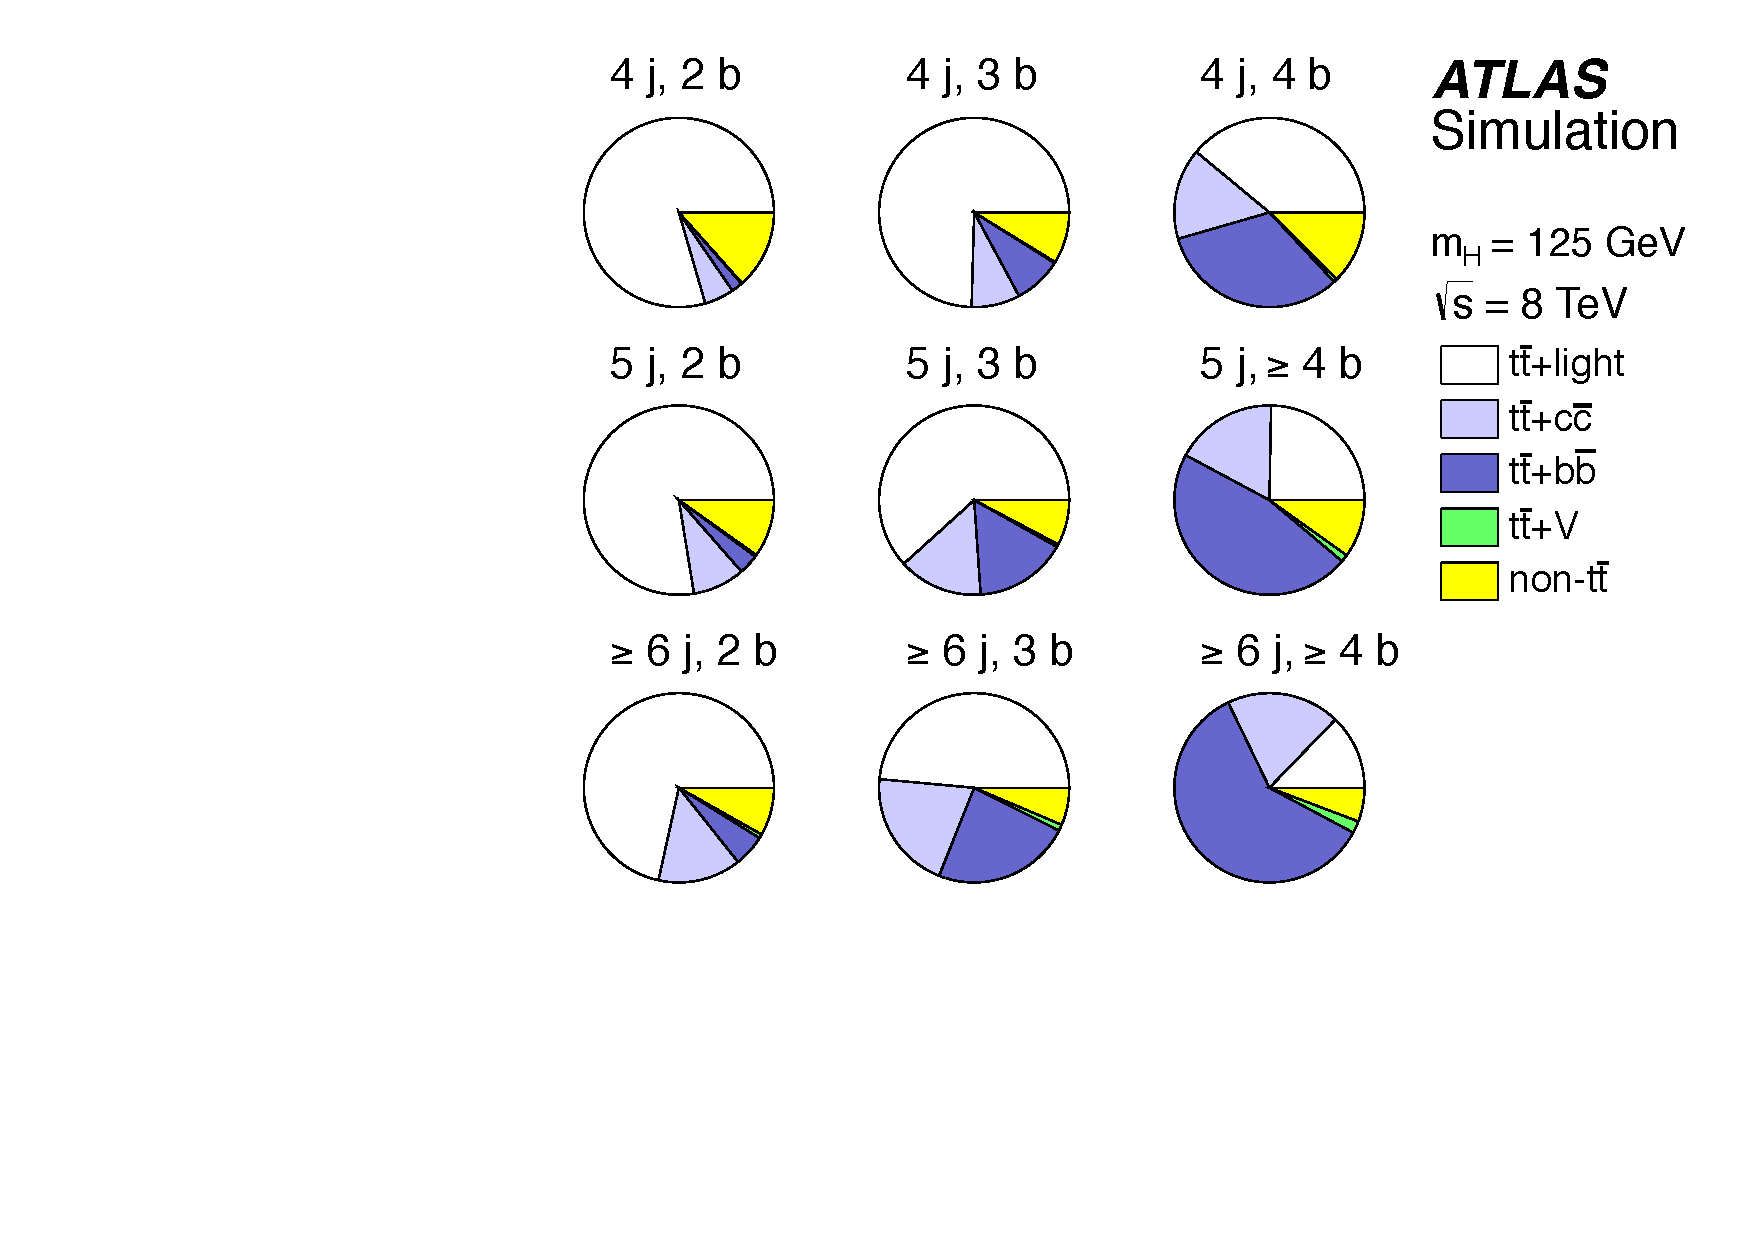
\includegraphics[width=0.75\textwidth]{Modeling/Figures/fig_02b_edit.pdf}
\caption{Fractional contributions of the various backgrounds to the total background
  prediction after preselection in each considered region. 
  Each row shows the plots for a
specific jet multiplicity (4, 5, $\geq$6), and the columns show the
$b$-jet multiplicity (2, 3, $\geq$4).
}
\label{fig:pie}
\end{figure}


\subsection{\texorpdfstring{\ttbar+jets background}{tt+jets background}}
The large phase space covered by the analyses requires a \ttbar\ simulation that describes correctly the different topologies, especially the emission of additional jets and the heavy-flavor fraction. 
Not only the normalization, but also
%In addition of a good prediction of the yields, 
the kinematics of the full final state have to be correctly modeled since several kinematic variables are used to build the final discriminants.
After several studies, it has been observed that \PP\ is the MC generator that models best \ttbar\ production. However, some corrections are needed to improve its prediction; these are described in the following sections.
The \ttbar\ sample is generated using the \powheg\ NLO generator~\cite{powheg,powbox1,powbox2} 
with the {\sc CT10} PDF set~\cite{ct101,ct102}. It is 
interfaced to {\sc Pythia} 6.426~\cite{Sjostrand:2006za} with the {\sc CTEQ61L}~\cite{cteq6} set of parton 
distribution functions and the Perugia2011C~\cite{Skands:2010ak} underlying event tune.  
The sample is normalized to the theoretical \xsec\ calculated at 
next-to-next-to leading order (NNLO) accuracy in QCD.
The calculation includes resummation of next-to-next-to-leading logarithmic (NNLL) soft-gluon terms 
with {\sc top++2.0}~\cite{ref:xs1,ref:xs2,ref:xs3,ref:xs4,ref:xs5,ref:xs6} yielding 
$\unit[253^{+15}_{-16}]{pb}$ for $\sqrt{s}=\unit[8]{\tev}$. 

The \ttbar+jets sample is generated inclusively and events are classified into three orthogonal samples: \ttbar+light-jets, \ttbb\ and \ttcc, according to the flavor of the additional jets.
The classification is based on an algorithm matching hadrons to particle jets built from stable particles as defined in section~\ref{sec:JetReco}.
First, the set of $b$- and $c$-hadrons with $\pT > \unit[5]{\gev}$ and not originating from \ttbar\ decay products is considered. This excludes hadrons originating from $b$-quarks from top decays, as well as hadrons produced by $c$-quarks from hadronic $W$ boson decays.
All particle jets with \pt\ $> \unit[15]{\gev}$ and $|\eta| < 2.5$ are  matched to the set of $b/c$-hadrons, if the matching satisfies $\DR < 0.4$ then the particle jet is labeled as a $b$- or $c$-jet. 
The \pt\ threshold for particle jets ($\unit[15]{\gev}$) is chosen to be \unit[10]{\gev} below the reconstructed-jet threshold, in order to allow for resolution effects.
Events with at least one $b$-jet not originated from top decay products are labeled as a \ttbb\ event. Events that fail this criteria, and containing at least one $c$-jet not from a $W$ decay are labeled as \ttcc. The set of \ttbb\ and \ttcc\ events will be referred to as \ttHF\ events, with HF standing for heavy flavor. 
The remaining events are labeled as \ttbar+light-jets events, including those with no jets in addition to the \ttbar\ decay products.

In order to perform more detailed studies of the \ttHF\ modeling and the related systematic uncertainties, a refined categorization is introduced. 
This categorization makes use of the number of heavy hadrons and particle jets in the event, as well as the details of the matching.
Further subcategories of the \ttbb\ and \ttcc\ samples are defined as follows.
If the event has only one particle jet matched to a $b$-hadron, the event is labeled
as \ttb.  If the event has two particle jets matched to two different $b$-hadrons, the event is labeled as \ttbb.  
If the event has one particle jet matched to two $b$-hadrons, the event is given the label \ttB, representing unresolved
gluon splitting to \bbbar. The same classification is performed in the \ttcc\ sample.

A duplication of the notation is unfortunately introduced, where \ttbb\ is used to refer both to the category of events with at least one additional $b$-jet, as well as the subcategory with two resolved $b$-jets. The context of the studies will hopefully make clear what it refers to, nevertheless, explicit clarification is included when needed.

\subsubsection{\texorpdfstring{\ttbar+light-jets modeling}{tt+light-jets modeling}}
The large amount of \ttbar\ events produced at the LHC has allowed a very detailed study of the kinematics of top production, through the measurement of differential \xsecs\ with the \unit[7]{\tev} data sample~\cite{Aad:2014zka}.
Among other observables,
differential \xsecs\ have been measured as a function of the
top-quark transverse momentum, \toppt, and the transverse
momentum of the \ttbar\ system, \ttbarpt.\footnote{ The top-quark kinematics are measured at the partonic level, after final-state radiation. This is equivalent to the status code 3 in \pythia.}
The most notable feature is that the MC prediction for most generators, and in particular for \PP, overpredicts the
data at high \toppt\ and \ttbarpt,
leading to a visible difference not covered by the statistical and
systematical uncertainties of the measurement, as seen in figure~\ref{fig:diffxsec}.

\begin{figure}[!t]
\begin{center}
  \begin{subfigure}{0.49\textwidth}{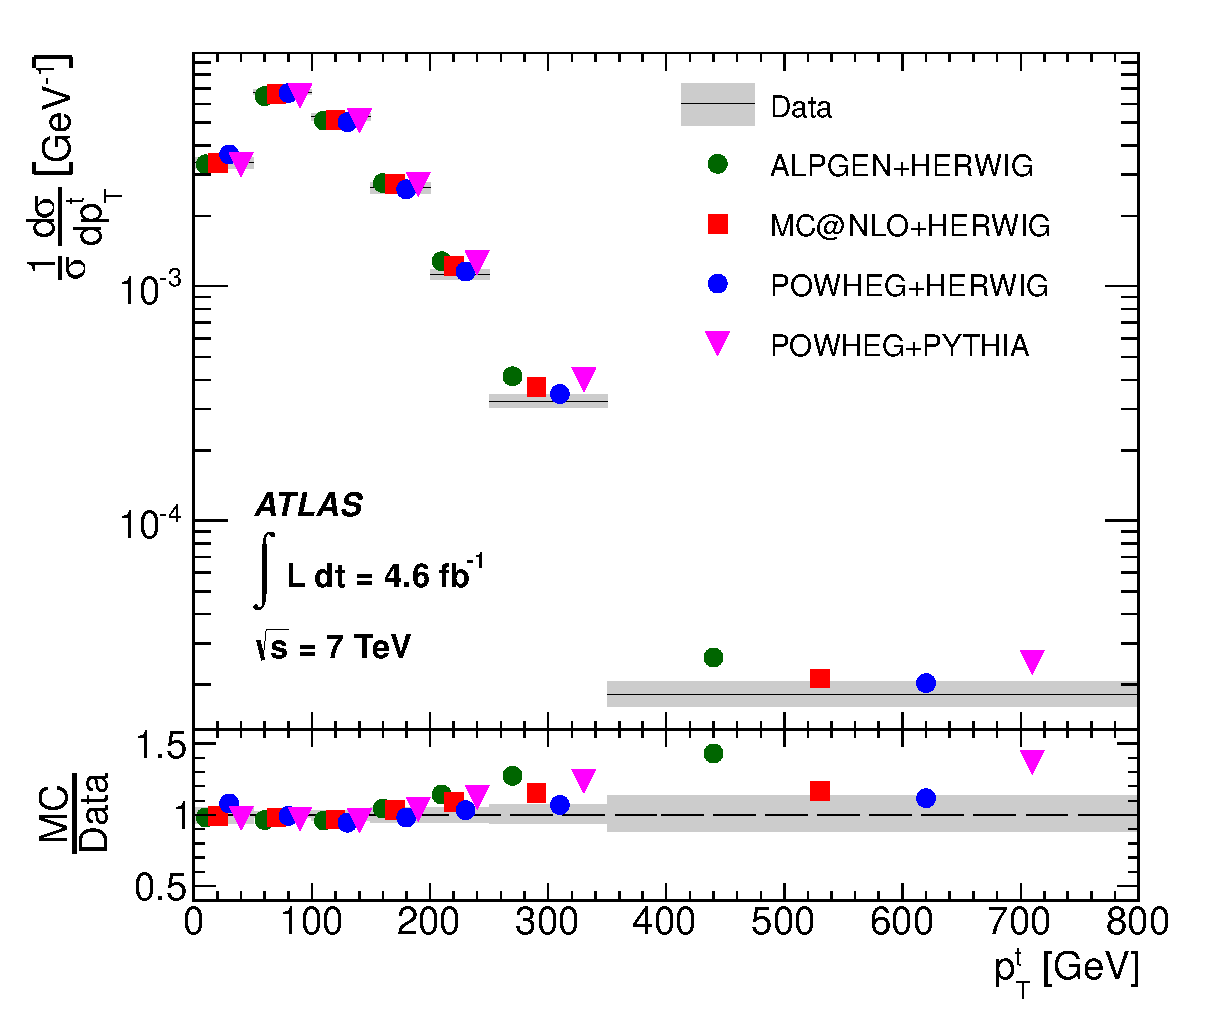
\includegraphics[width=\textwidth]{Modeling/Figures/fig_08a}}\label{fig:diffxsec_a}
    \end{subfigure}
  \begin{subfigure}{0.49\textwidth}{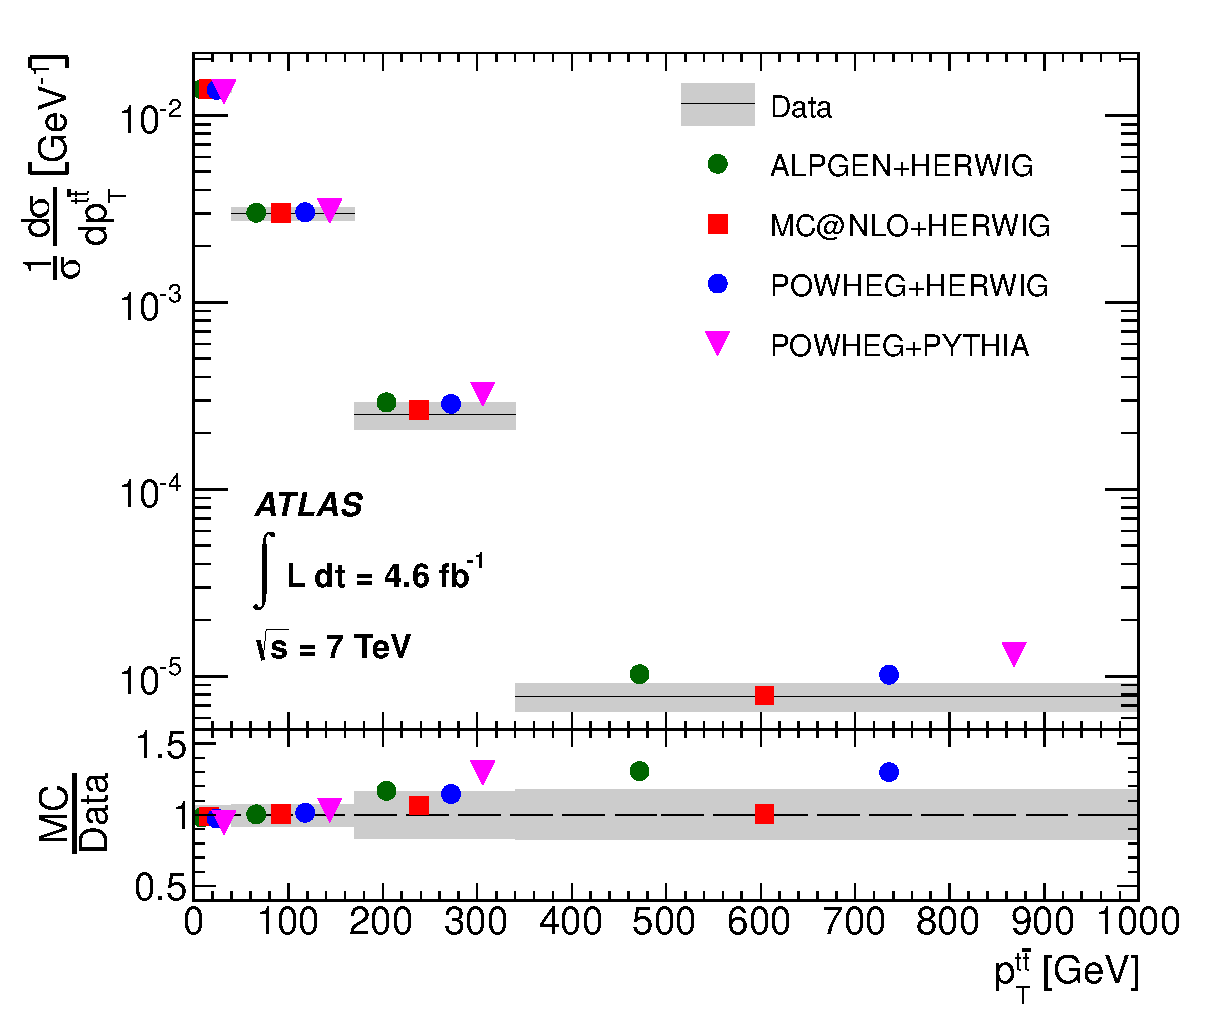
\includegraphics[width=\textwidth]{Modeling/Figures/fig_08c}}\label{fig:diffxsec_c}
    \end{subfigure} \\
\caption{
  Normalized differential \xsecs\ for the transverse momentum of the hadronically-decaying top quark, \toppt, and the transverse momentum of the \ttbar\ system, \ttbarpt. Generator predictions are shown as markers, with inverted triangles for \PP. The gray bands indicate the total uncertainty on the data in each bin. From reference~\cite{Aad:2014zka}. 
}
\label{fig:diffxsec}
\end{center}
\end{figure}

To correct for this effect, two reweighting factors are derived and their
product is applied as a multiplicative factor to each event
based on the value of top quark \pt\ and \ttbar\ system 
\pt, taking the correlation between these two parameters 
into account. 
First a reweighting factor based on \ttbarpt\ is derived, in order to bring
the \ttbarpt\ distribution in \PP\ in agreement with the differential \xsec\ measurement.
After applying this first reweighting factor, a second factor is derived to correct the \toppt\ distribution.
This two-step sequential procedure is needed in order to take into account the non-negligible correlation ($\sim \unit[30]{\%}$) between both variables.
Table~\ref{tab:PPfactors} summarizes the correction factors with the corresponding binning and the total uncertainties.

\begin{table}[bt!]
\centering

\begin{tabular}{ c c c c c}
\toprule
\toprule
\multicolumn{5}{c}{\ttbarpt}  \\
\midrule
Bins [\gev]                 &    [0, 40]                 &   [40, 170]             &  [170, 340]             &  [340, 1000)        \\ 
Rew. factor & 1.04 $\pm$ 0.12 &  0.99 $\pm$ 0.14 &  0.81 $\pm$ 0.18 & 0.68 $\pm$ 0.22 \\
\bottomrule
\bottomrule
\end{tabular}
\bigskip

  \makebox[\textwidth][c]{
\begin{tabular}{ c c c c c c c c}
\toprule
\toprule
\multicolumn{8}{c}{\toppt}  \\
\midrule
Bins [\gev]                 &    [0, 50]                   &   [50, 100]               &  [100, 150]              &  [150, 200]             &  [200, 250]              &  [250, 350]               &  [350, 800) \\ 
Rew. factor &  \small 1.01$\pm$0.01 & \small 1.01$\pm$0.02  & \small 1.01$\pm$0.01  & \small 1.00$\pm$0.01  & \small 0.96$\pm$0.04  & \small 0.91$\pm$0.09  & \small 0.88$\pm$0.17   \\ 
\bottomrule
\bottomrule

%Rew. factor & \small{ 1.01$\pm$0.01  & 1.01$\pm$0.02  & 1.01$\pm$0.01  & 1.00$\pm$0.01  & 0.96$\pm$0.04  & 0.91$\pm$0.09  & 0.88$\pm0.17 }  \\ 
\end{tabular}
}

\caption{
Reweighting factors for the \textsc{PowHeg+Pythia} sample as a function of the \ttbar\ system \pT\ (top) and the top quark \pT\ (bottom). The two factors are multiplied to obtain the event weight correction.}
\label{tab:PPfactors}
\end{table}

This reweighting procedure, which will be referred to as \ttbar\ reweighting, is applied inclusively to the three subsamples: \ttbar+light jets, \ttbb\ and \ttcc. 
The validity of applying this reweighting to \ttHF\ will be discussed in section~\ref{subsec:ttbb}.

Figure~\ref{fig:ttbarseqrw} shows the effect  of the reweighting procedure for \ttbar\ events on the data/MC agreement in regions with exactly two $b$-tagged jets,
which are dominated by the \ttbar+light-jets background.
An improvement in the data description is clearly visible in the jet multiplicity and the scalar sum of the jet \pt\ (\hthad) distributions.
The former is driven by the \ttbarpt\ component of the correction while the latter is mainly due to the correction as a function of the top quark \pT.

\begin{figure}[!tp]
\begin{center}
  \begin{subfigure}{0.49\textwidth}{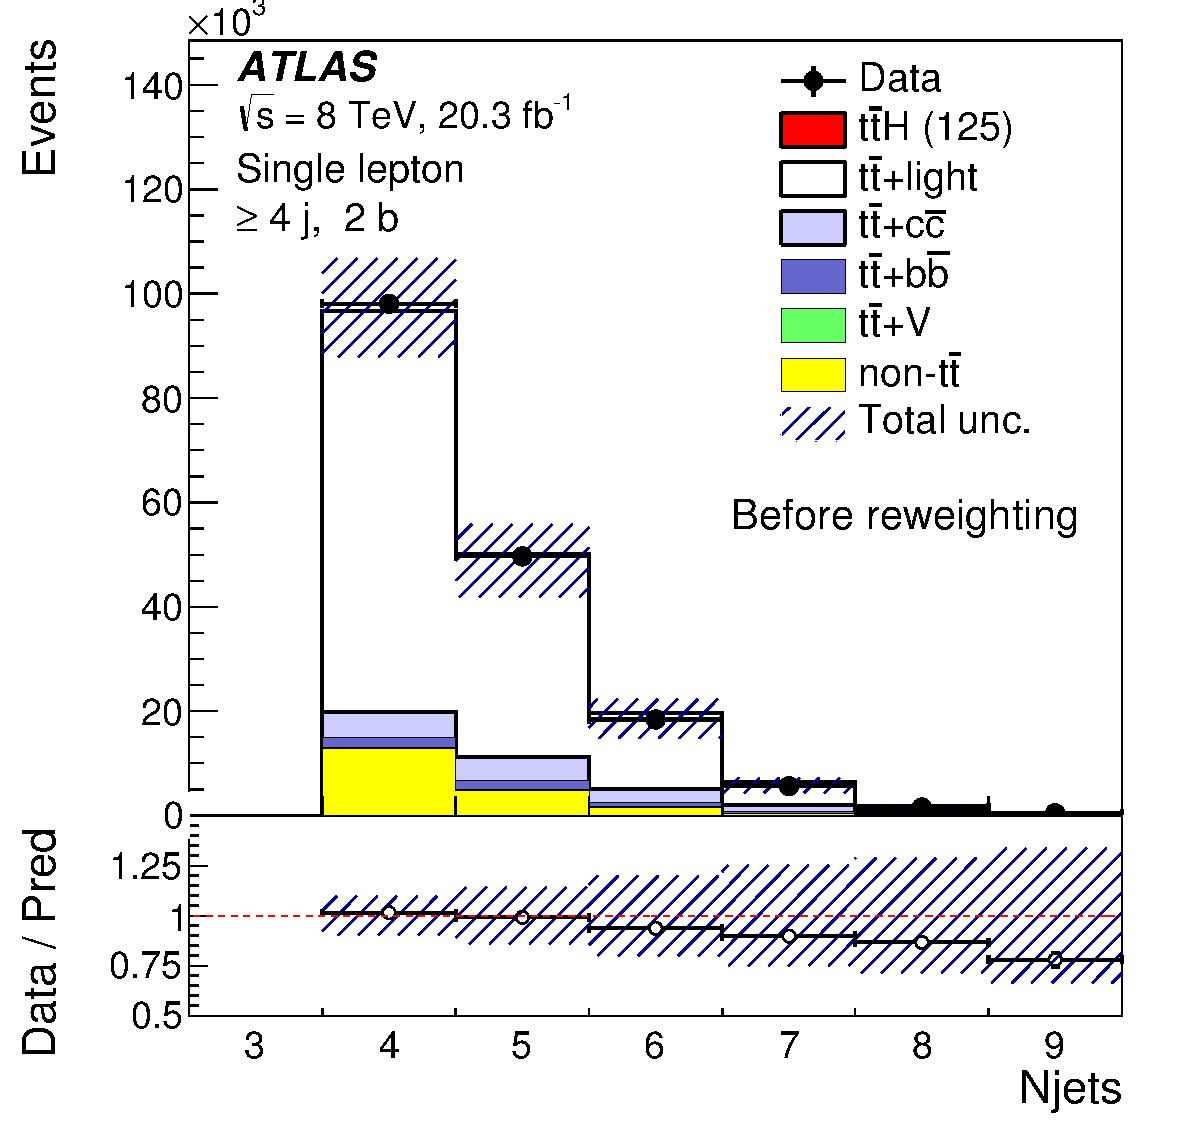
\includegraphics[width=\textwidth]{Modeling/Figures/fig_05a.pdf}}\label{fig:ttbarseqrw_a}
    \caption{}\end{subfigure}
  \begin{subfigure}{0.49\textwidth}{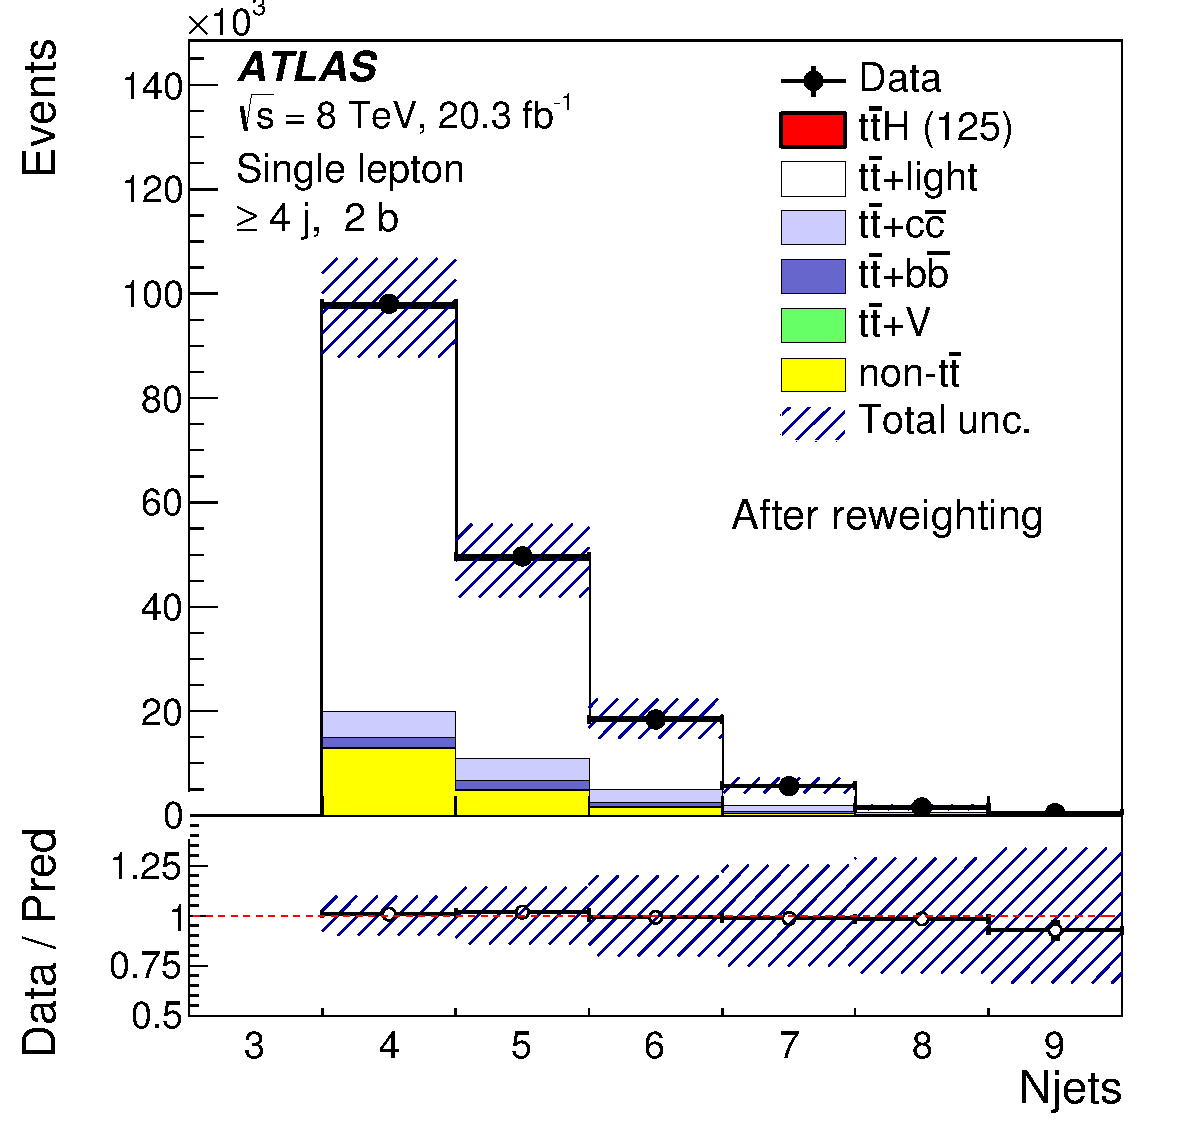
\includegraphics[width=\textwidth]{Modeling/Figures/fig_05b.pdf}}\label{fig:ttbarseqrw_b}
    \caption{}\end{subfigure} \\
  \begin{subfigure}{0.49\textwidth}{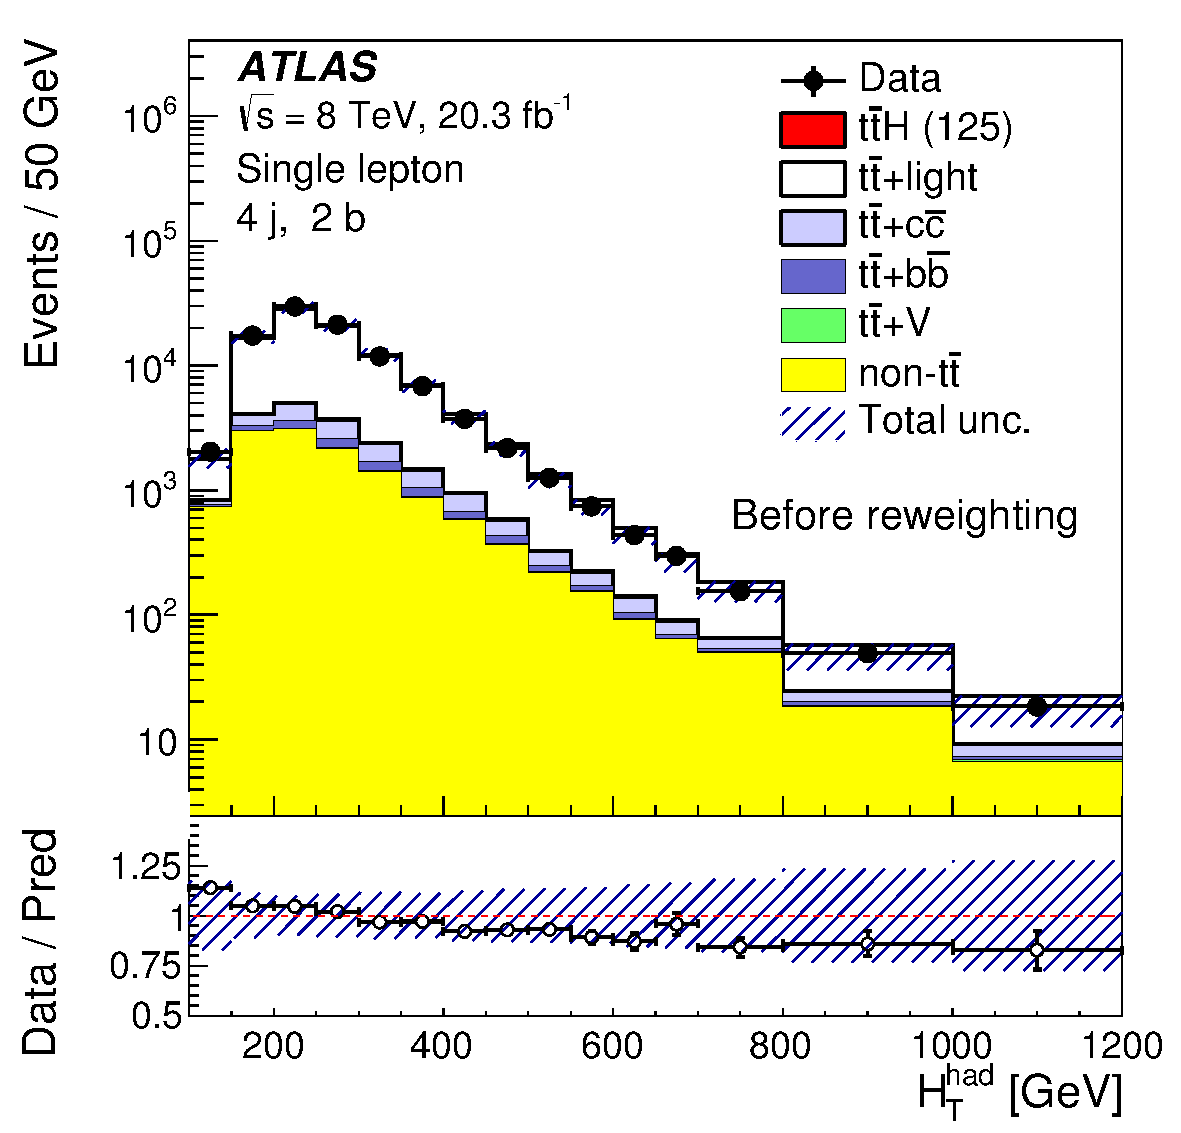
\includegraphics[width=\textwidth]{Modeling/Figures/fig_05c.pdf}}\label{fig:ttbarseqrw_c}
    \caption{}\end{subfigure}
  \begin{subfigure}{0.49\textwidth}{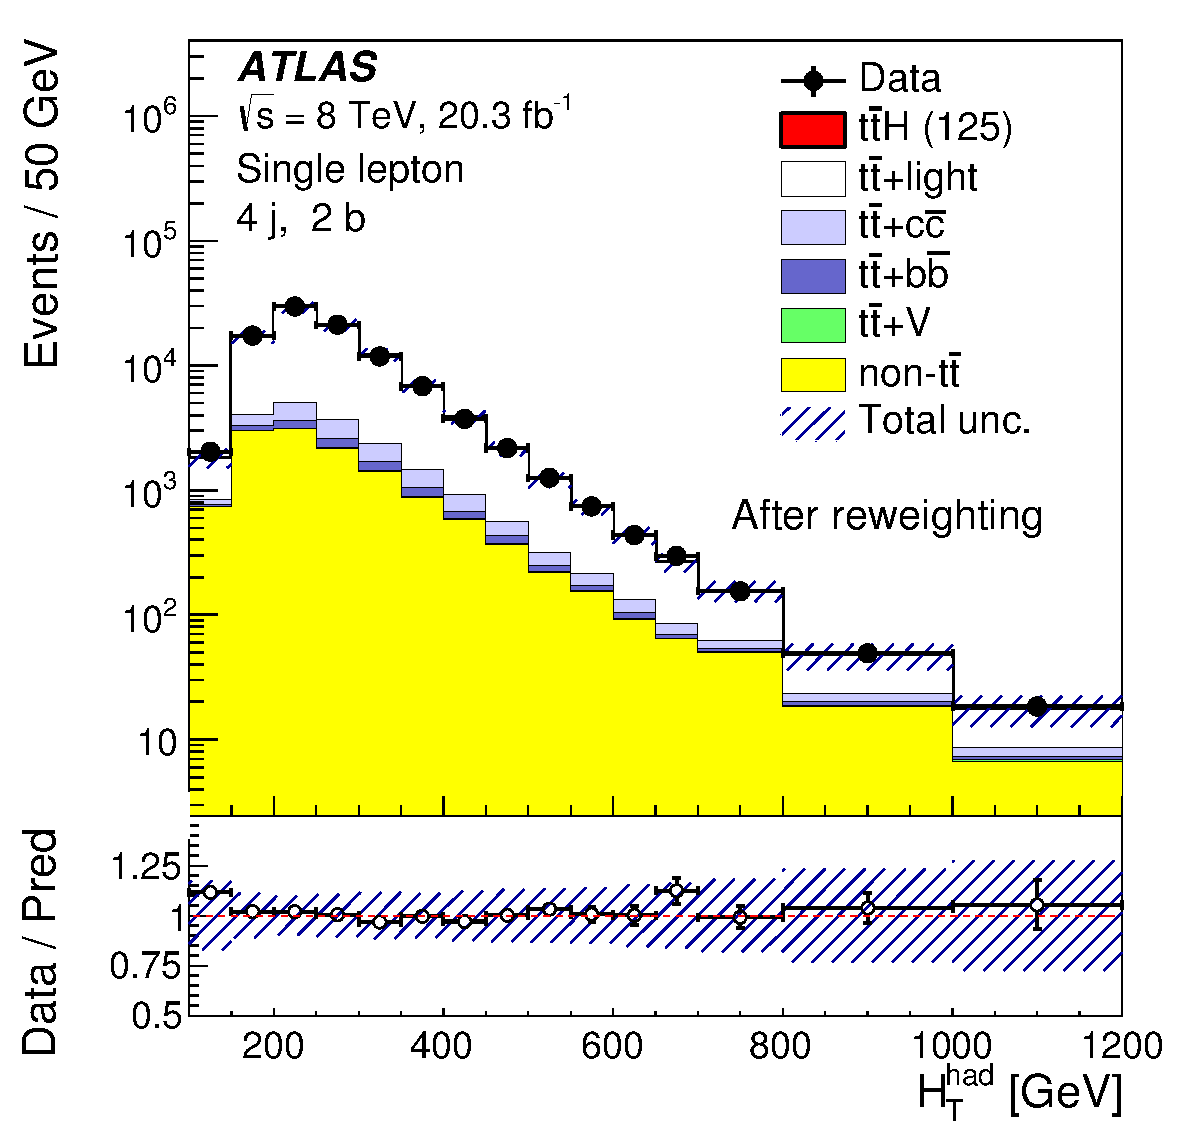
\includegraphics[width=\textwidth]{Modeling/Figures/fig_05d.pdf}}\label{fig:ttbarseqrw_d}
    \caption{}\end{subfigure}
\caption{The exclusive 2-$b$-tag region before and after the reweighting of the \pt\ of the \ttbar\ system and the \pt\ of the top quark of the \textsc{Powheg+Pythia} $t\bar{t}$\ sample.
The jet multiplicity distribution (a) before and (b) after the reweighting;  
\hthad\ distributions (c) before and (d) after the reweighting. }
\label{fig:ttbarseqrw}
\end{center}
\end{figure}


\subsubsection{\texorpdfstring{\ttbb\ modeling}{ttbb modeling}}
\label{subsec:ttbb}
The main irreducible background in the signal regions is \ttbb\ production, therefore a precise modeling of this process is of uttermost importance. 
Fixed-order NLO calculations for \ttbb\ production can reduce perturbative
uncertainties on the \xsec\ from \unit[70-80]{\%} of the LO calculation, down to \unit[15-20]{\%}~\cite{Bredenstein:2009aj,Bredenstein:2010rs,Bevilacqua:2009zn}. 
NLO predictions with massive $b$-quarks matched to a parton shower have also become available recently~\cite{Cascioli:2013era}.

In the \powheg\ generator only diagrams of the type $gb\rightarrow \ttbar b$ are directly included, while the production of \bbbar\ pairs is obtained with the parton shower, therefore the modeling of \ttbb\ has only leading-logarithmic (LL) accuracy. In order to study and improve the \ttbb\ modeling, different MC generators are tested and compared to \PP. 

An inclusive \ttbar\ sample is generated with the \madgraphfive\ 1.5.11 generator~\cite{Alwall:2011uj}, using the {\sc CT10} PDF set and interfaced to \pythia\ 6.427 for showering and hadronization. It includes tree-level diagrams with up to three extra partons, including $b$- and $c$-quarks. A five-flavor scheme is used, where $b$- and $c$-quarks are treated as massless partons in the ME calculation and can be originated inside the proton.

A state-of-the-art NLO prediction with massive $b$-quarks and matched to a parton shower is also available
within the {\sc Sherpa} framework, interfaced with the {\sc OpenLoops} library~\cite{Gleisberg:2008ta,Cascioli:2011va}. % referred to in the following as \ShOL. 
The \ShOL\ NLO sample is generated 
following the four-flavor scheme using the {\sc Sherpa} 2.0 pre-release and  
the {\sc CT10} PDF set. In the four-flavor scheme the $b$-quark does not contribute to the proton PDF, 
and can only be generated as a massive final state.
The renormalization scale ($\mu_{\rm R}$) is set to   
$\mu_{\rm R}=\prod_{i=t,\bar{t},b,\bar{b}}E_{\mathrm{T},i}^{1/4} $, 
where $E_{\mathrm{T},i}$ 
is the transverse energy of parton $i$, and the  
factorization and resummation scales are both set 
to $\mu_{\rm F}=\mu_{\rm Q}=(E_{\mathrm{T}, t }+E_{\mathrm{T}, \bar{t} })/2$.  
The ME is then interfaced to the \sherpa\ parton shower.

In contrast to \madgraph\ and \powheg, where an inclusive \ttbar\ sample is generated, the \ShOL\ sample is an exclusive \ttbb\ sample. However, the presence of massive $b$-quarks in the generation allows the computation to cover the full \ttbb\ phase space, including collinear gluon splitting into \bbbar. 
For the sake of completeness, it has to be noted that there is a small contribution of \ttbb\ --like diagrams not included in the \ShOL\ sample.
First, \bbbar\ pairs arising from multiple parton interaction (MPI) overlaying \ttbar+jets events. And second, the production of a \bbbar\ pair from a gluon radiated off the top decay products, which will be labeled as final-state radiation (FSR). Example Feynman diagrams for these contributions are shown in figure~\ref{fig:ttbb_noSherpa}.
These two contributions, MPI and FSR, have to be identified and excluded from the comparison to the \ShOL\ sample.

\begin{figure}[!tp]
\begin{center}
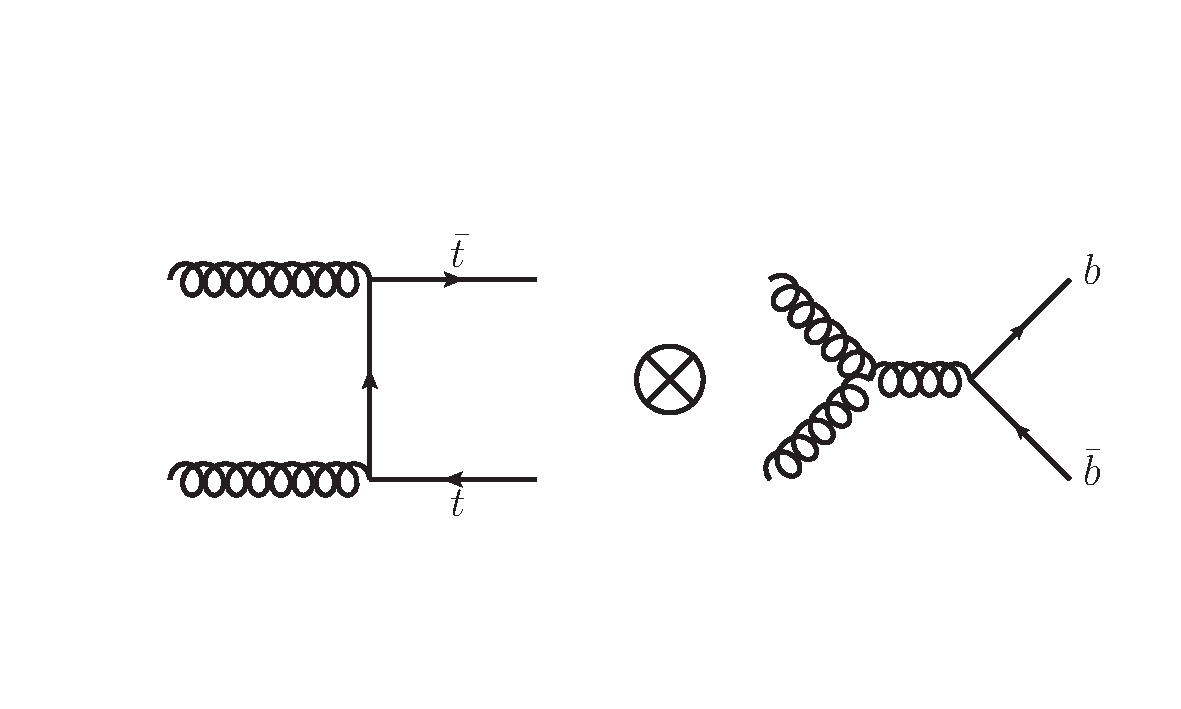
\includegraphics[width=0.75\textwidth]{Modeling/Figures/ttbb_MPI_good} \\
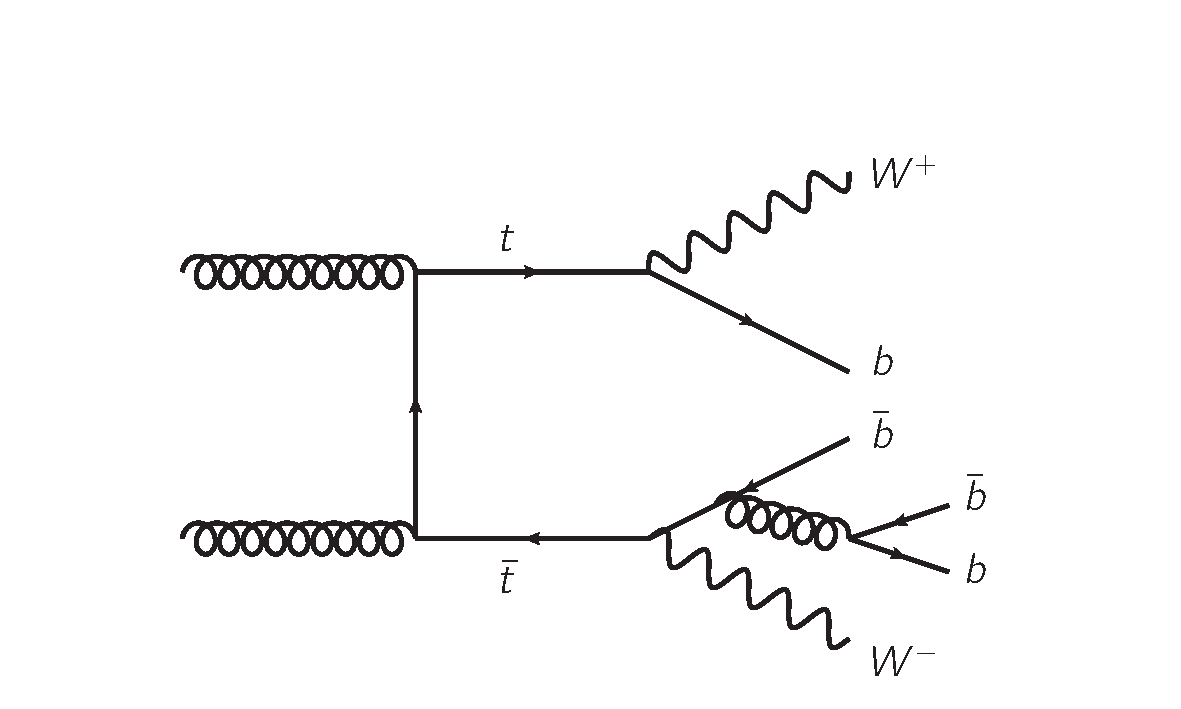
\includegraphics[width=0.75\textwidth]{Modeling/Figures/ttbb_FSR_good}
\caption{\bbbar\ production from multiple parton interaction overlayed with a \ttbar\ event from the hard scatter (top) and final state radiation (bottom).}
\label{fig:ttbb_noSherpa}
\end{center}
\end{figure}

The absolute contribution of the various $\ttbar+\geq 1$ $b$ particle-jet topologies to the \xsec\ is shown in 
figure~\ref{fig:default_extHFtype}. 
A difference in the inclusive \ttbb\ \xsec\ is observed, with the \powheg\ prediction being about \unit[20]{\%} above \ShOL.
The relative distribution across categories is such that \ShOL\ predicts higher 
contribution of the $t\bar{t}+B$ category, 
as well as every category where the production of a second pair of \bbbar\ is required. 

\begin{figure}[!tbp]
\begin{center}
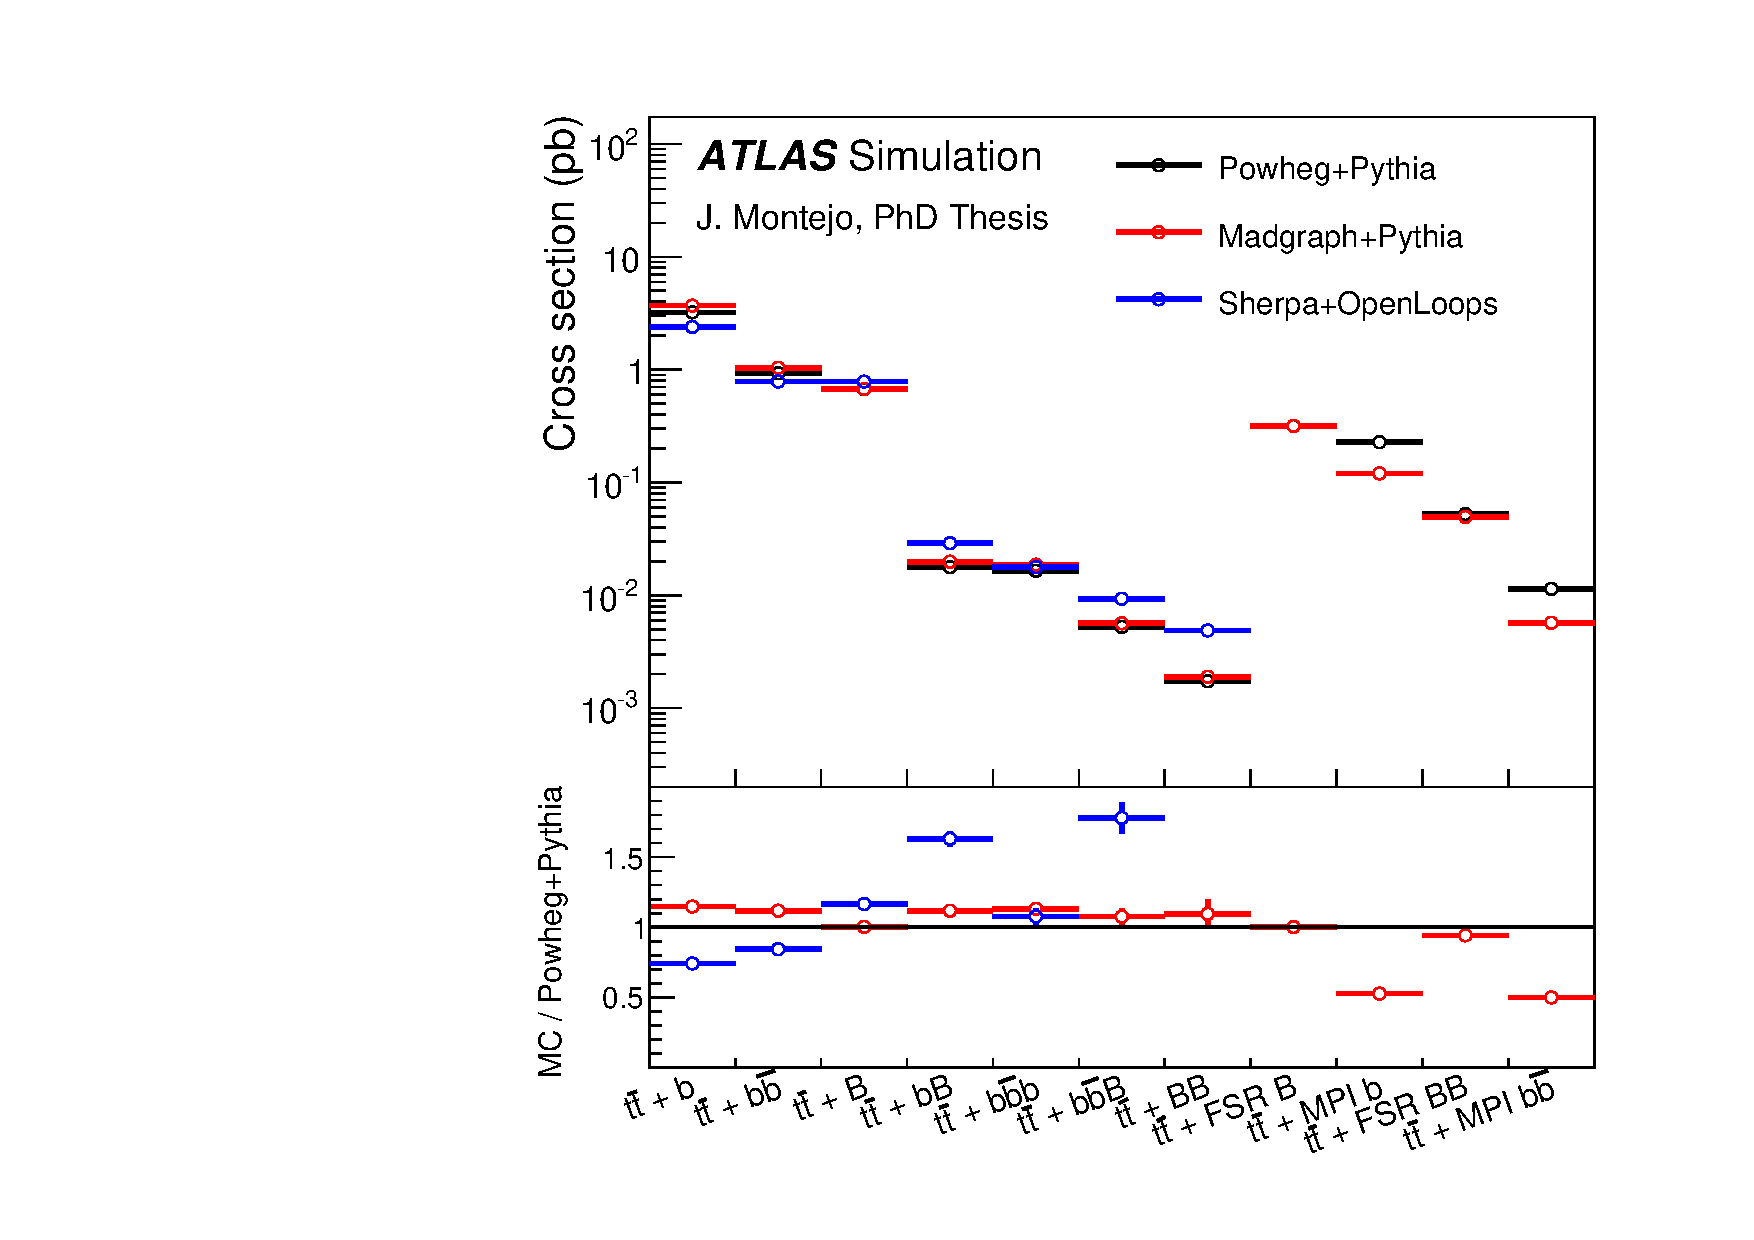
\includegraphics[width=0.7\textwidth]{Modeling/Figures/default_realHFbb_extHFtype}
\caption{Comparison of \ttbb\ subcategories between \PP, \madgraph+\pythia\ and \ShOL.}
\label{fig:default_extHFtype}
\end{center}
\end{figure}

Some examples of normalized distributions of different relevant variables across categories are shown in 
figure~\ref{fig:default_example}, and the full set of figures can be found in appendix~\ref{app:ttbb_modeling}.
The modeling of the relevant kinematic variables in each category is in reasonable agreement between \powheg\ (after top-quark \pt\ and \ttbar\ \pt\ reweighting)
and NLO \ttbb. Some differences are observed in the \ttbarpt\ and $\DR^{\bbbar}$ distributions. Good agreement is also found between \PP\ and \madgraph+\pythia. Since the production of \bbbar\ pairs in \PP\ originates only from the parton shower, the agreement could be a product of using the same showering program, \pythia, in both samples. Some studies are performed to validate the agreement between generators and can be found in appendix~\ref{app:ttbb_modeling}.

\begin{figure}[tp!]
\begin{center}
\begin{tabular}{cc}
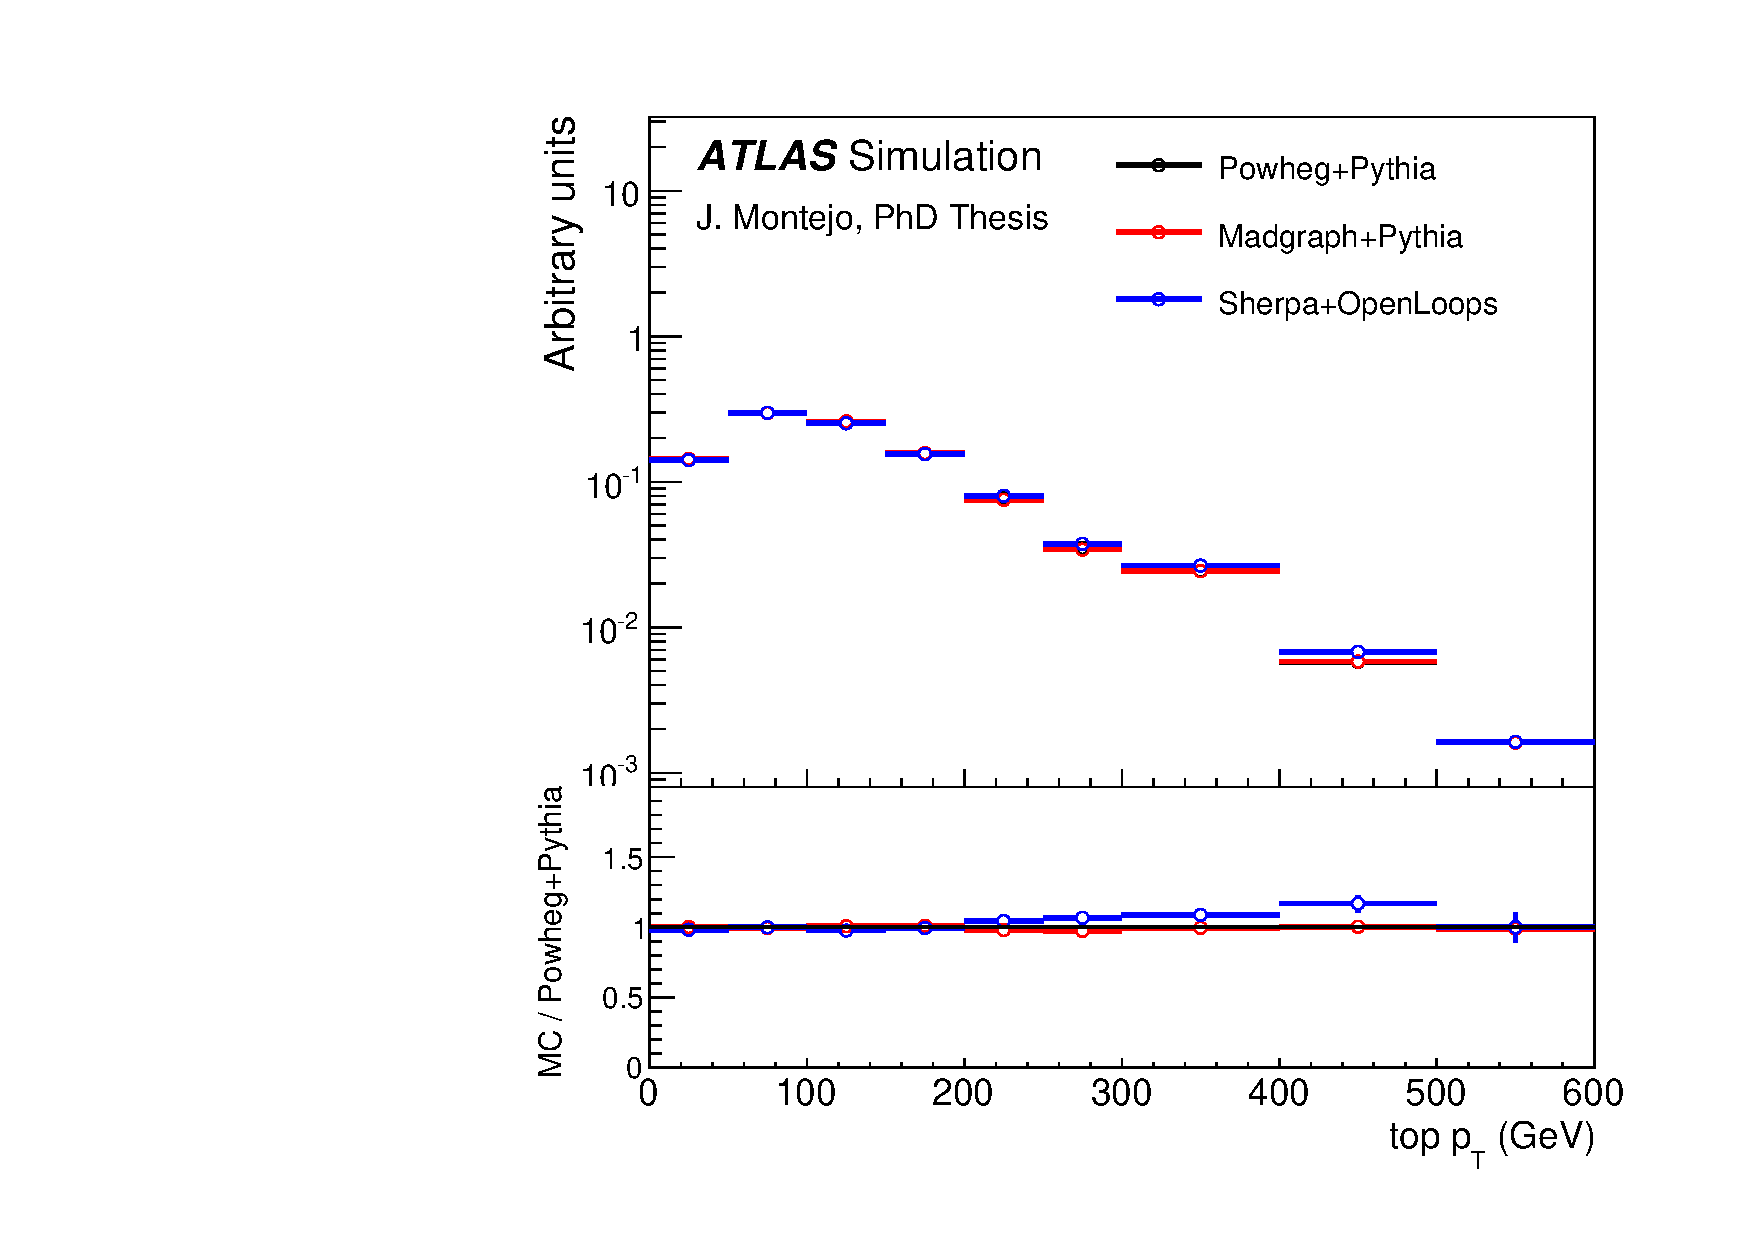
\includegraphics[width=0.48\textwidth]{Modeling/Figures/default_tt1bq_top_pt_norm} &
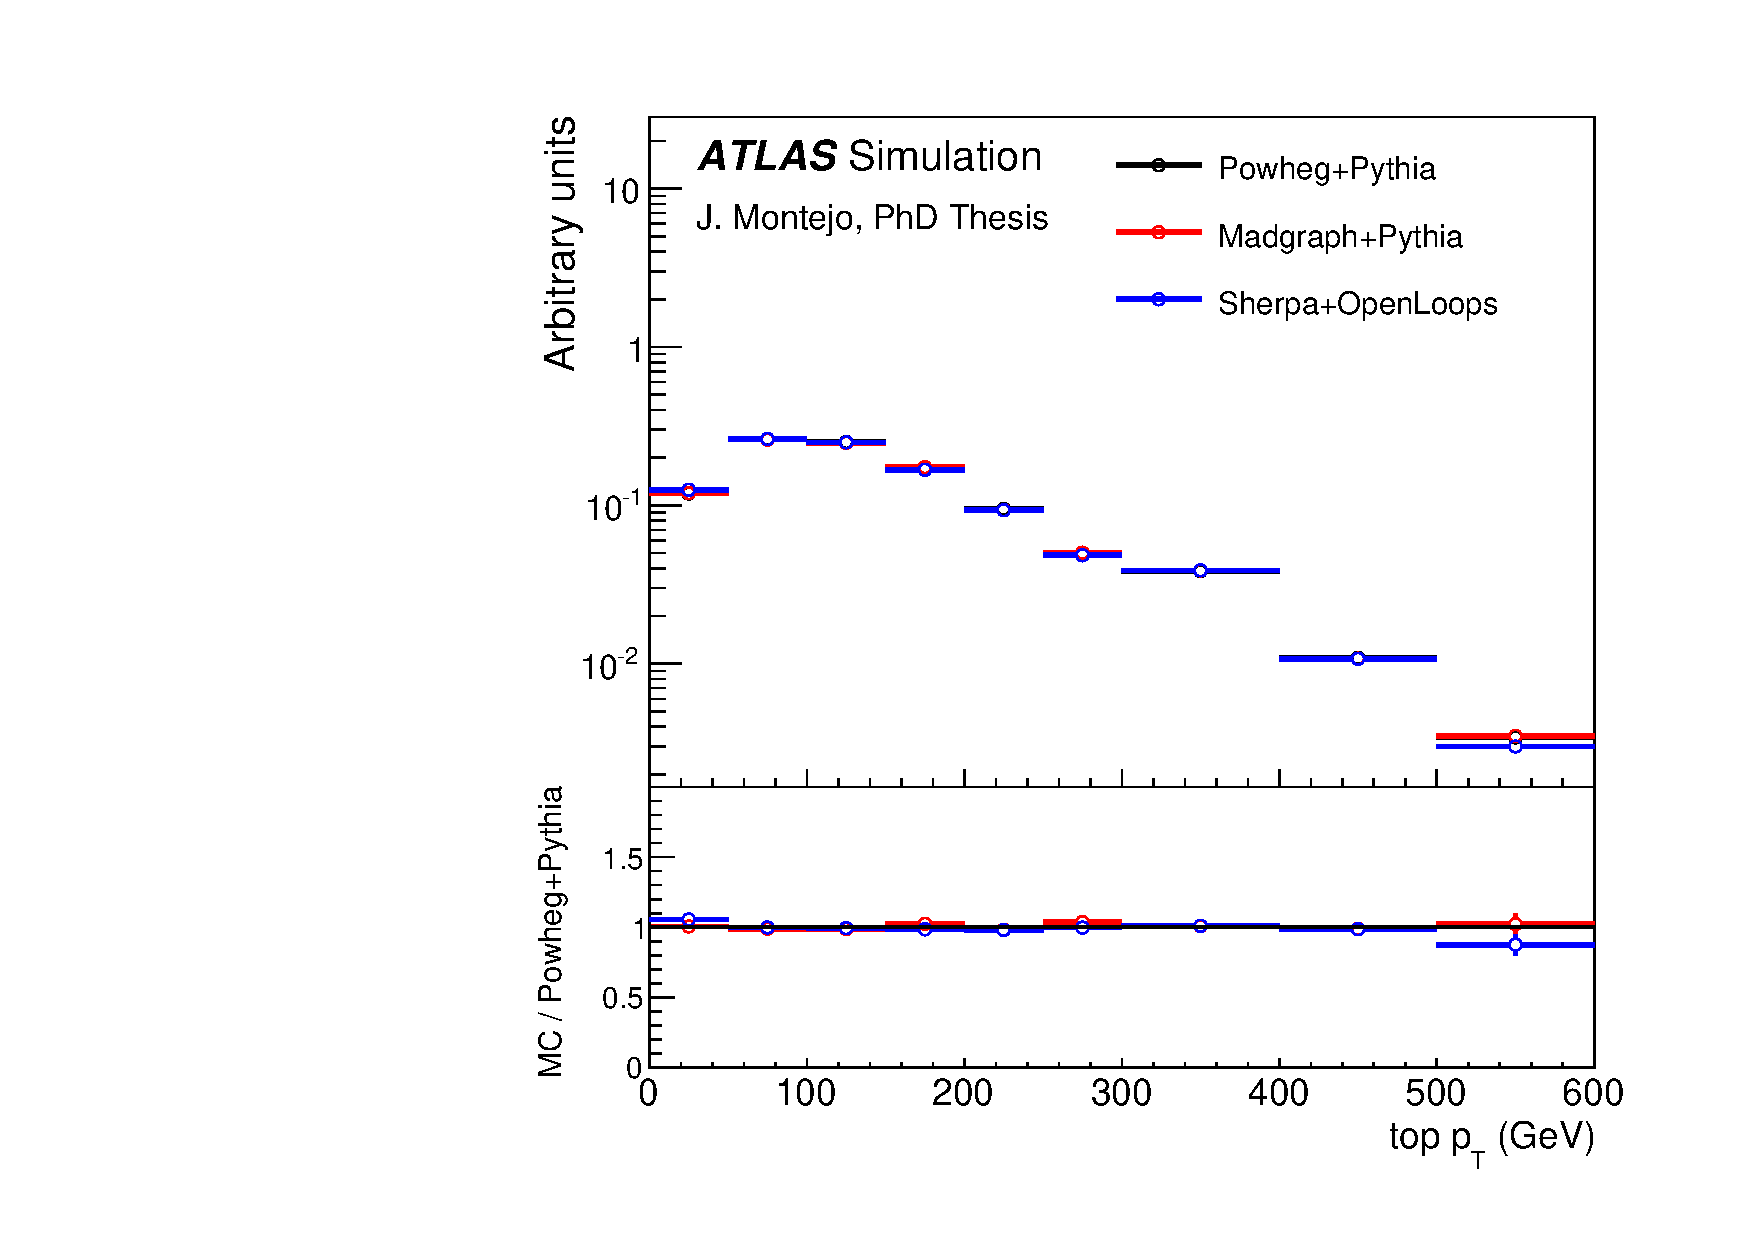
\includegraphics[width=0.48\textwidth]{Modeling/Figures/default_tt1gbbq_top_pt_norm} \\
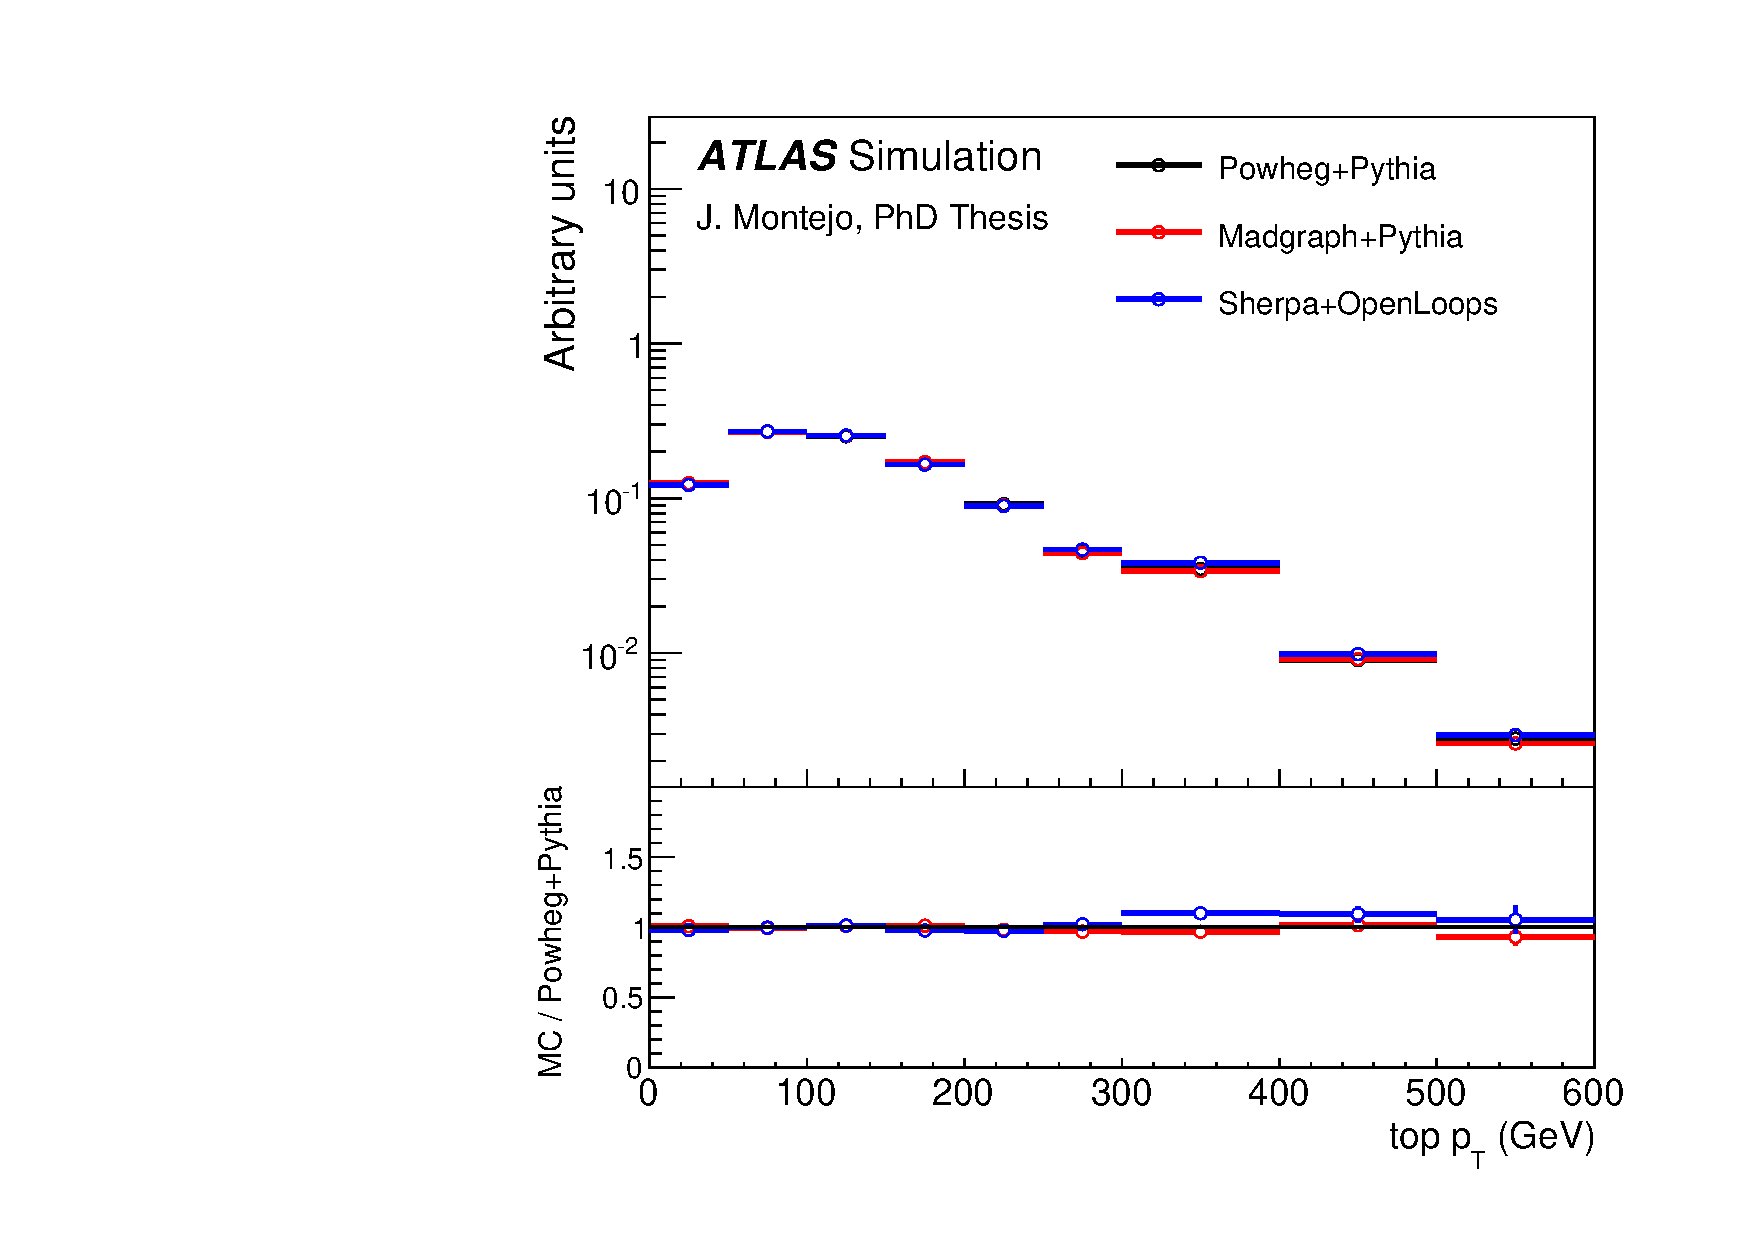
\includegraphics[width=0.48\textwidth]{Modeling/Figures/default_tt2bq_top_pt_norm} &
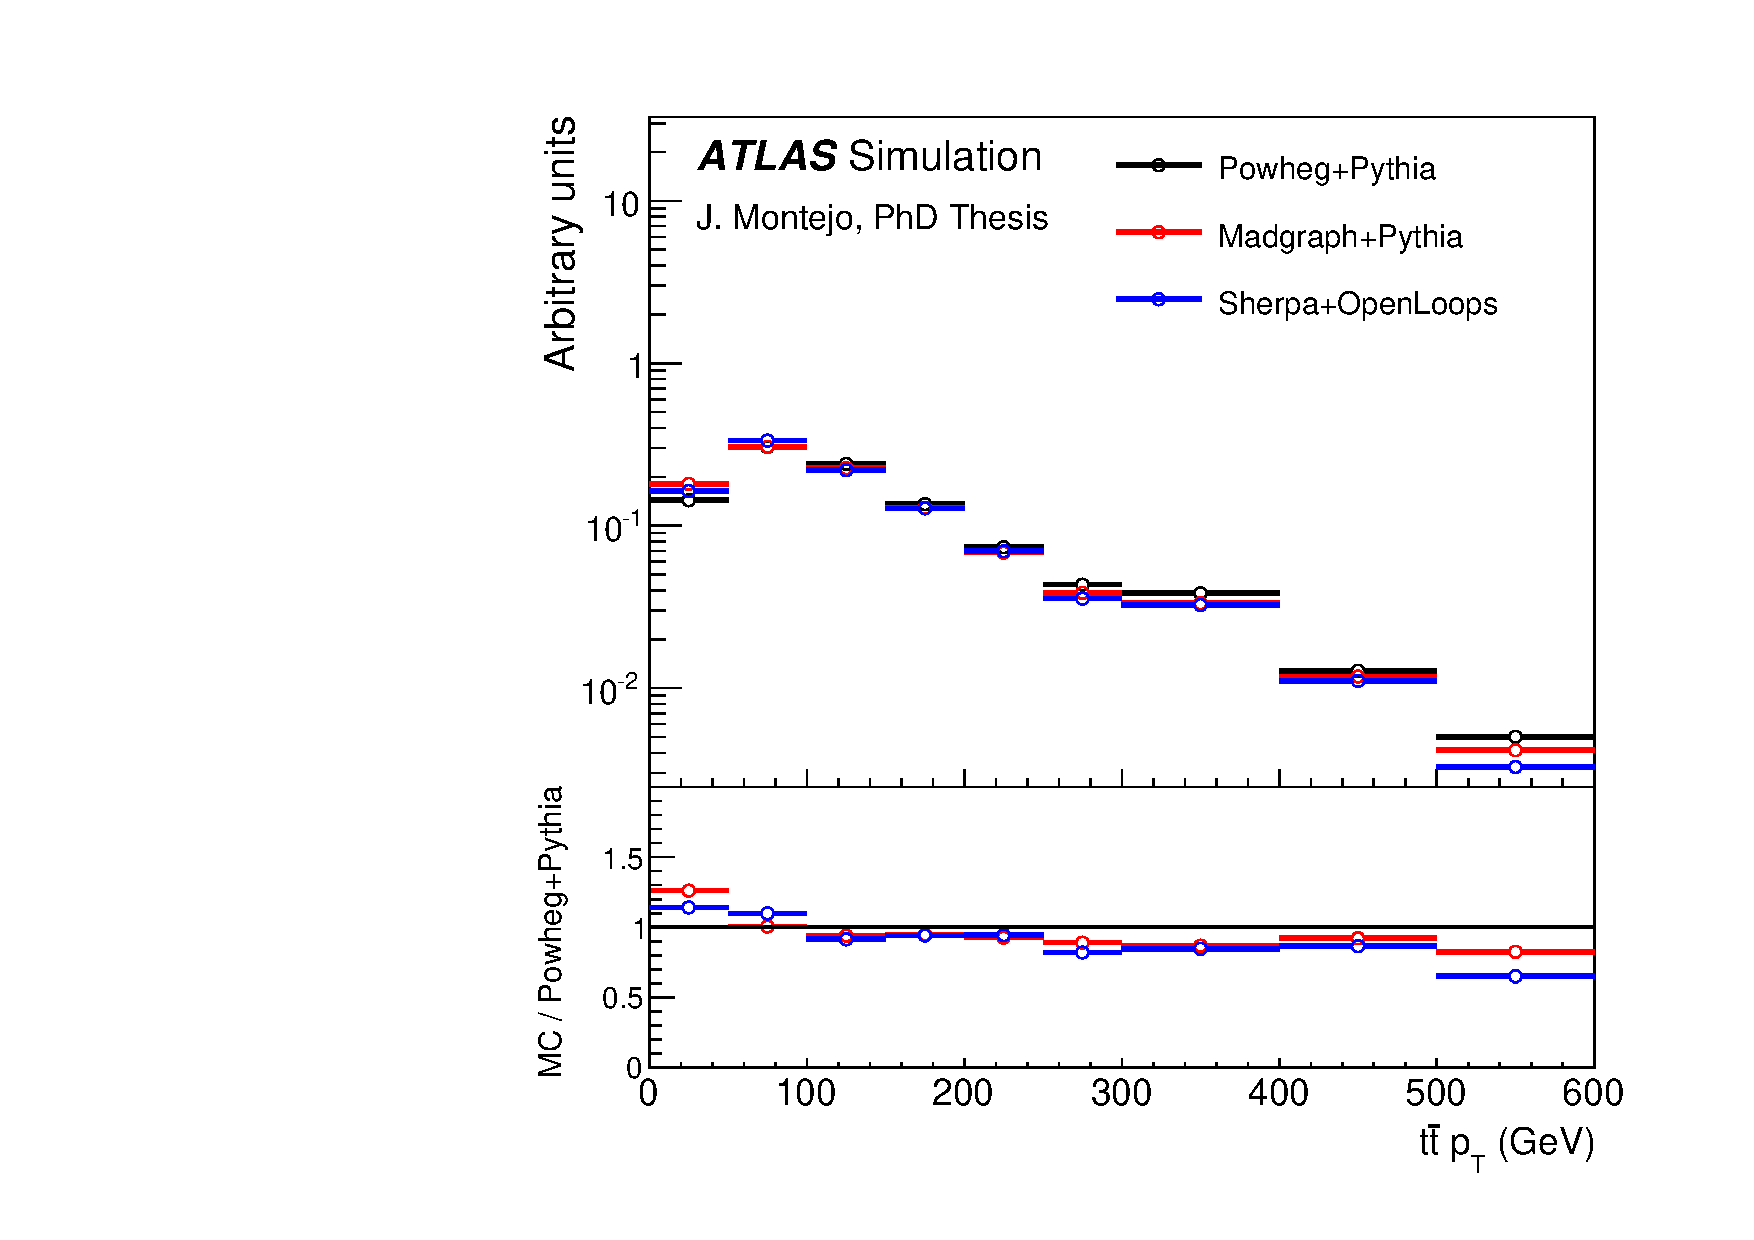
\includegraphics[width=0.48\textwidth]{Modeling/Figures/default_tt2bq_ttbar_pt_norm} \\
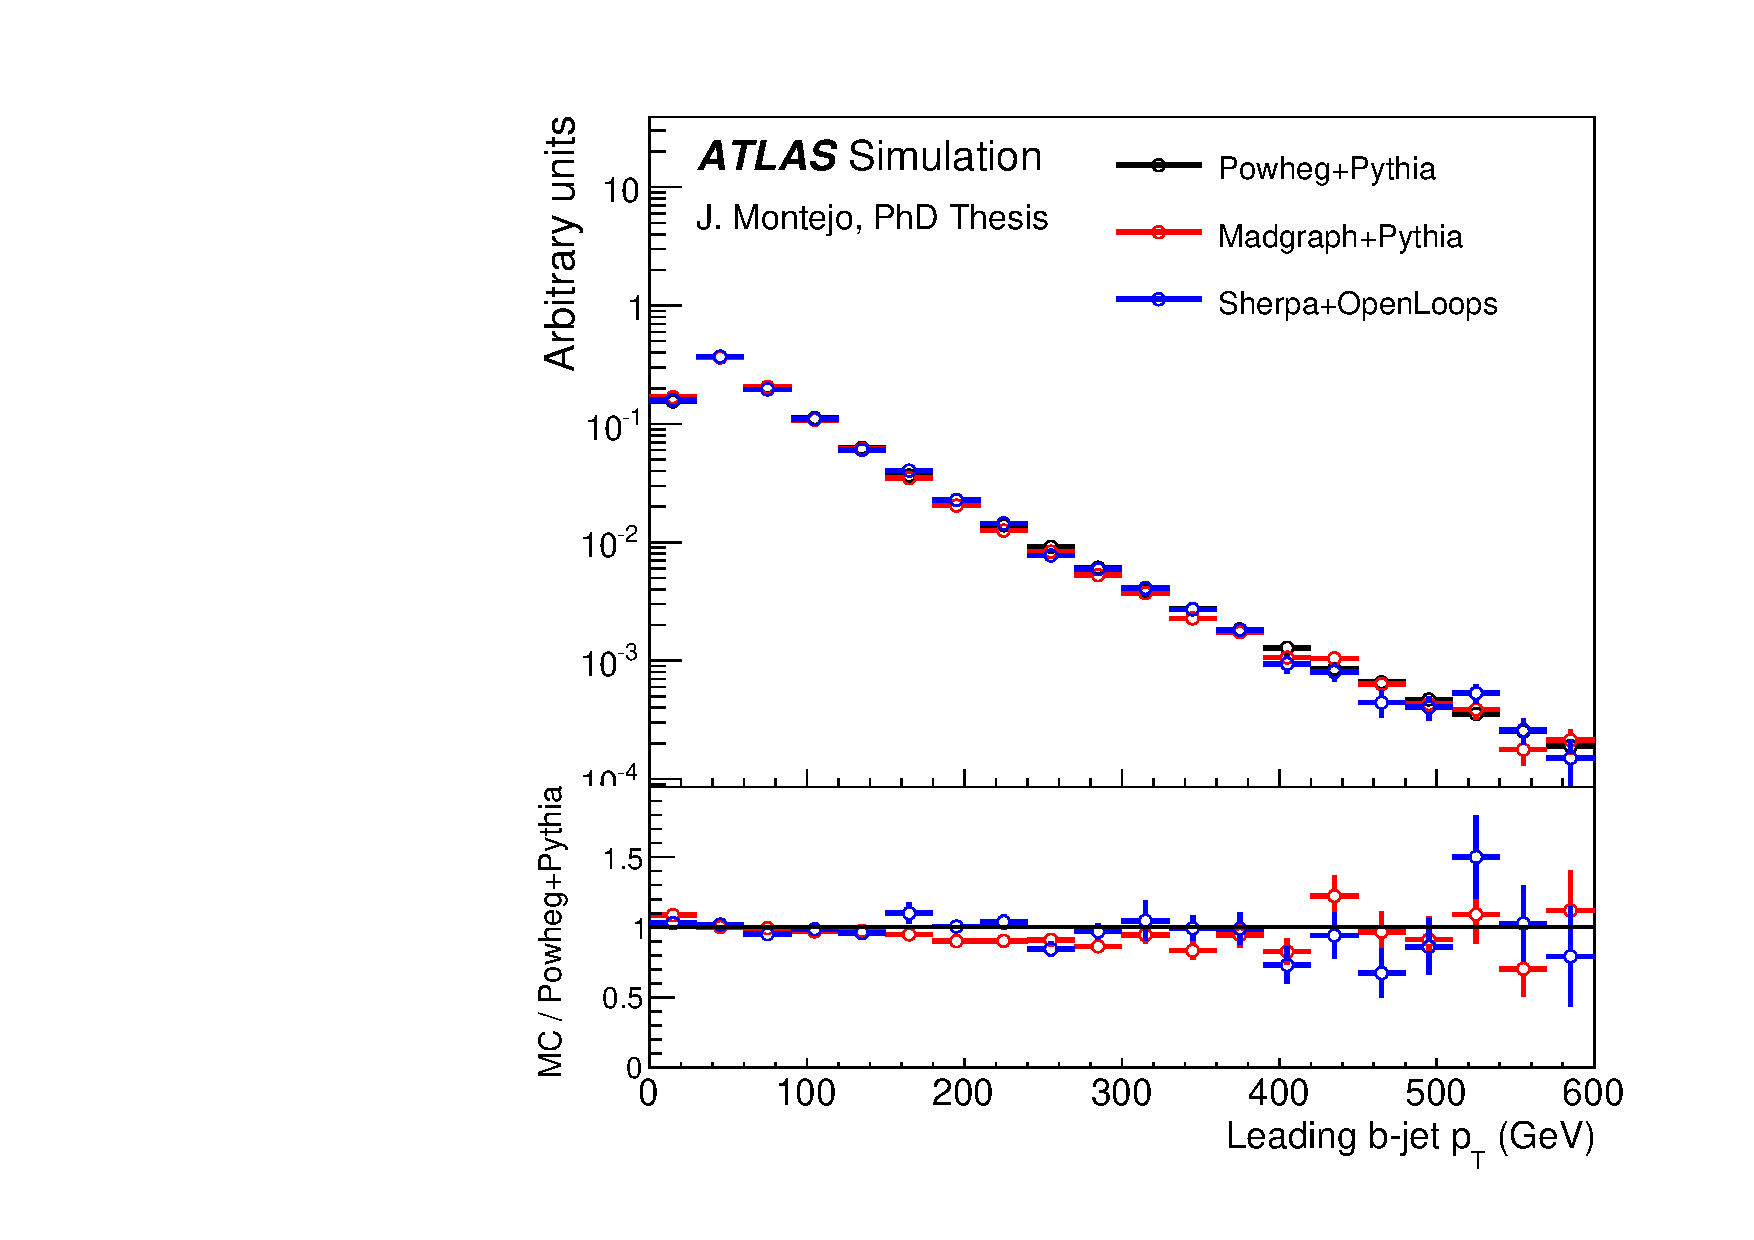
\includegraphics[width=0.48\textwidth]{Modeling/Figures/default_tt2bq_q1_pt_norm} &
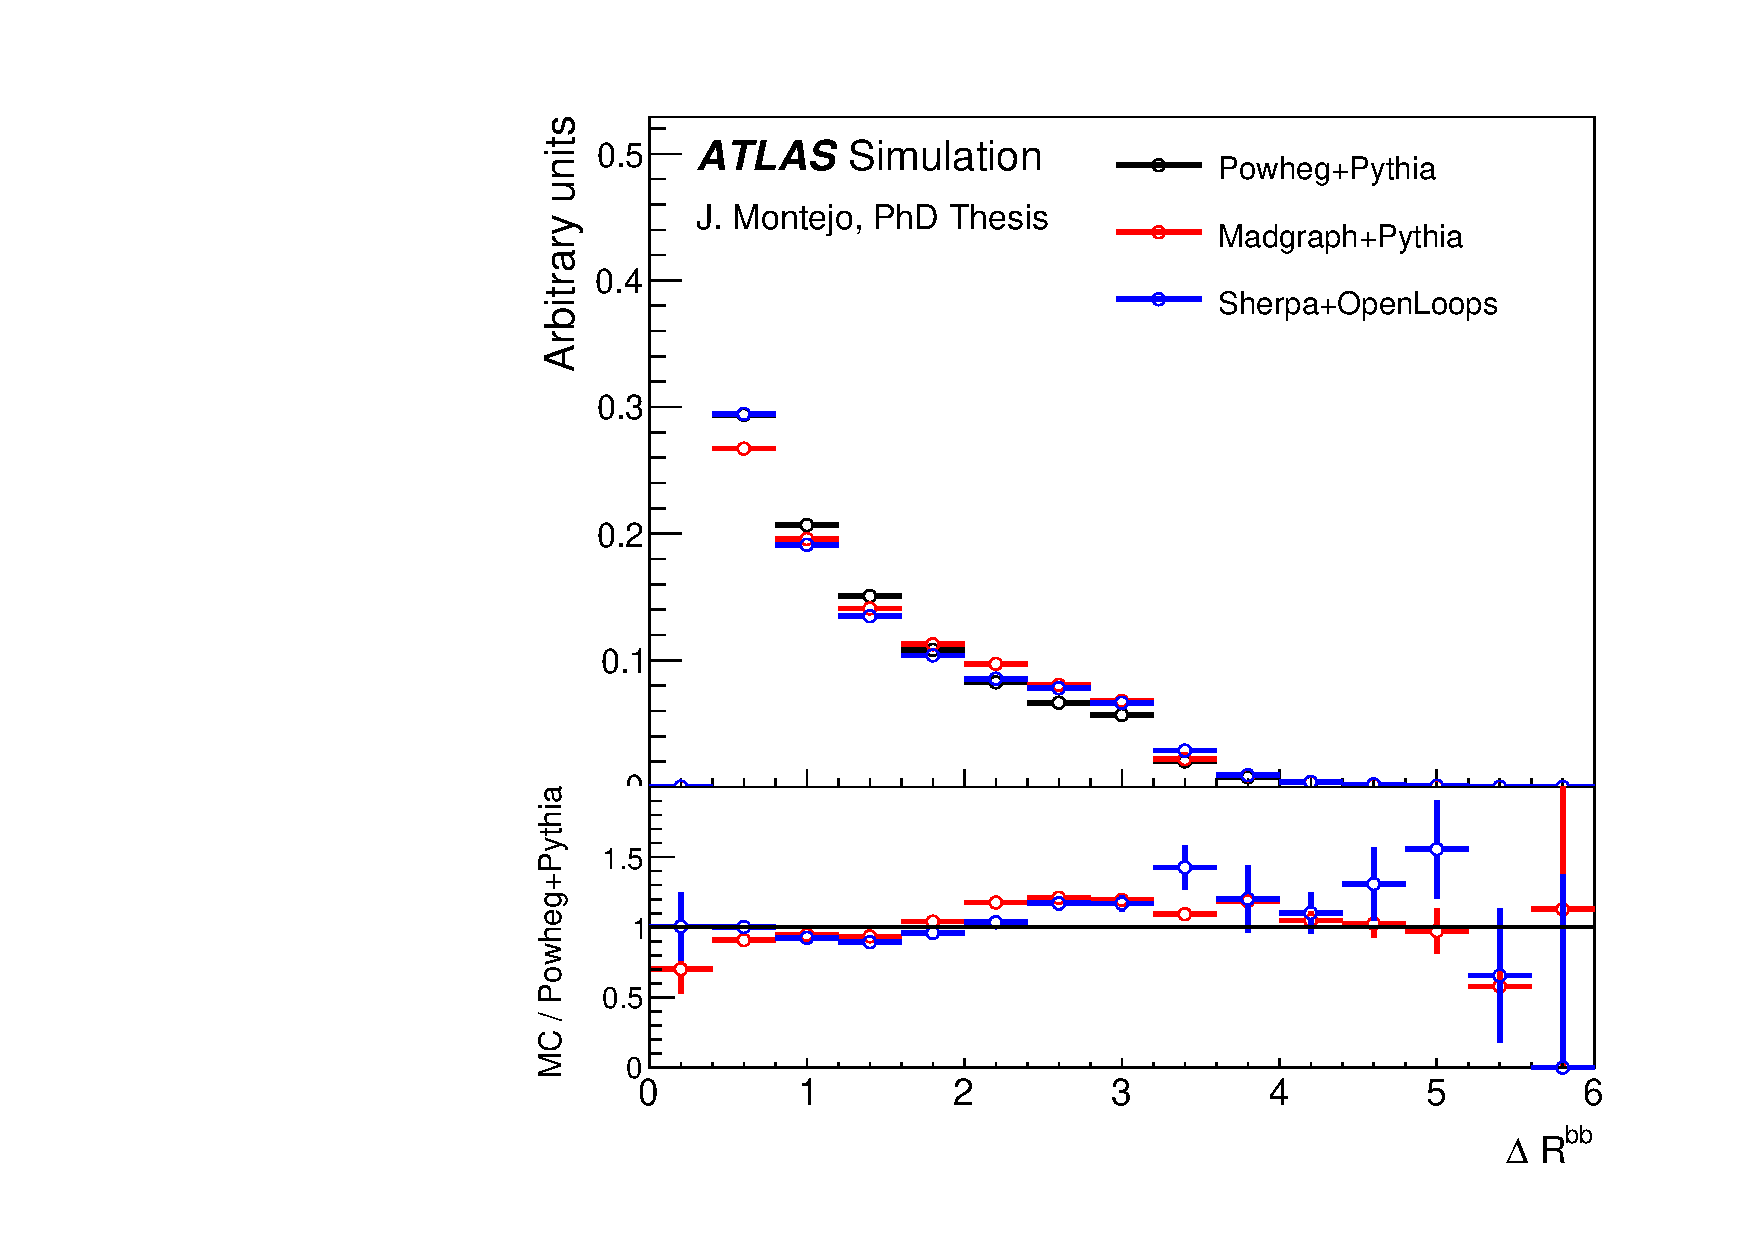
\includegraphics[width=0.48\textwidth]{Modeling/Figures/default_tt2bq_qq_dr_norm} \\
\end{tabular}
\caption{Comparison of kinematic variables in different topologies: \toppt\ in \ttb\ (top left), \toppt\ in \ttB\ (top right), \toppt\ in \ttbb\ (middle left), \ttbarpt\ in \ttbb\ (middle right), leading $b$-jet \pt\ in \ttbb\ (bottom left) and $\DR^{\bbbar}$ in \ttbb\ (bottom right).}
\label{fig:default_example}
\end{center}
\end{figure}

The \ttbar\ reweighting derived from the differential \xsec\ measurement is applied inclusively on the three \ttbar\ categories. 
The reweighting of the \ttHF\ component is in principle difficult to justify since the differential \xsec\ measurement is dominated by \ttbar+light jets. 
In \ttbb\ this reweighting is in fact redundant since it could be absorbed in the NLO reweighting. Nevertheless, it is possible to compare the sample before and after \ttbar\ reweighting with the NLO calculation. As it can be seen in figure~\ref{fig:ttreweighting_ttbb}, the \ttbar\ reweighting applied to the \ttbb\ sample improves the agreement with the NLO prediction. %, and the residual difference is corrected by the \ttbb\ NLO reweighting. 
This is taken as an indication that the reweighting is also applicable to the \ttHF\ component, and in particular to \ttcc, for which no NLO prediction exists.

\begin{figure}[!tp]
\begin{center}
  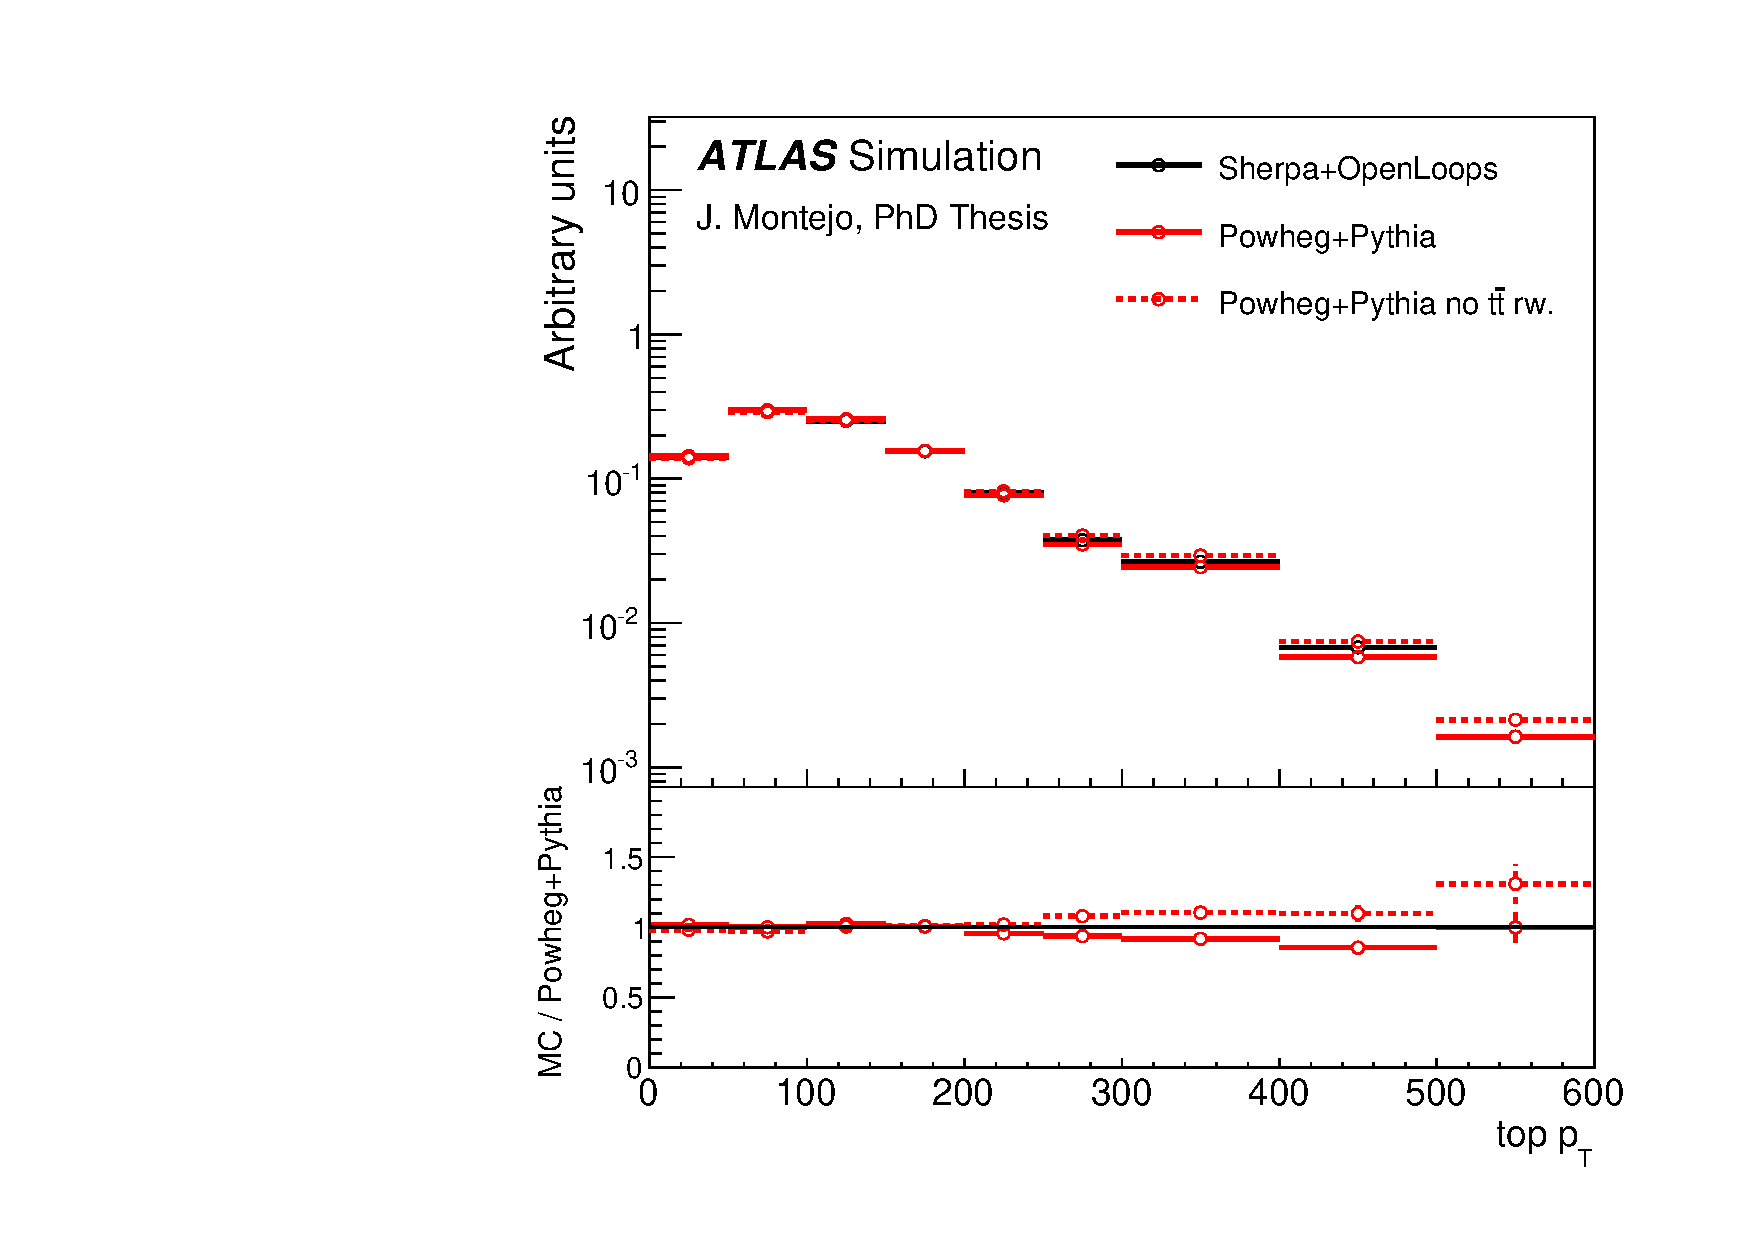
\includegraphics[width=0.46\textwidth]{Modeling/Figures/norw_tt1bq_top_pt_norm}
  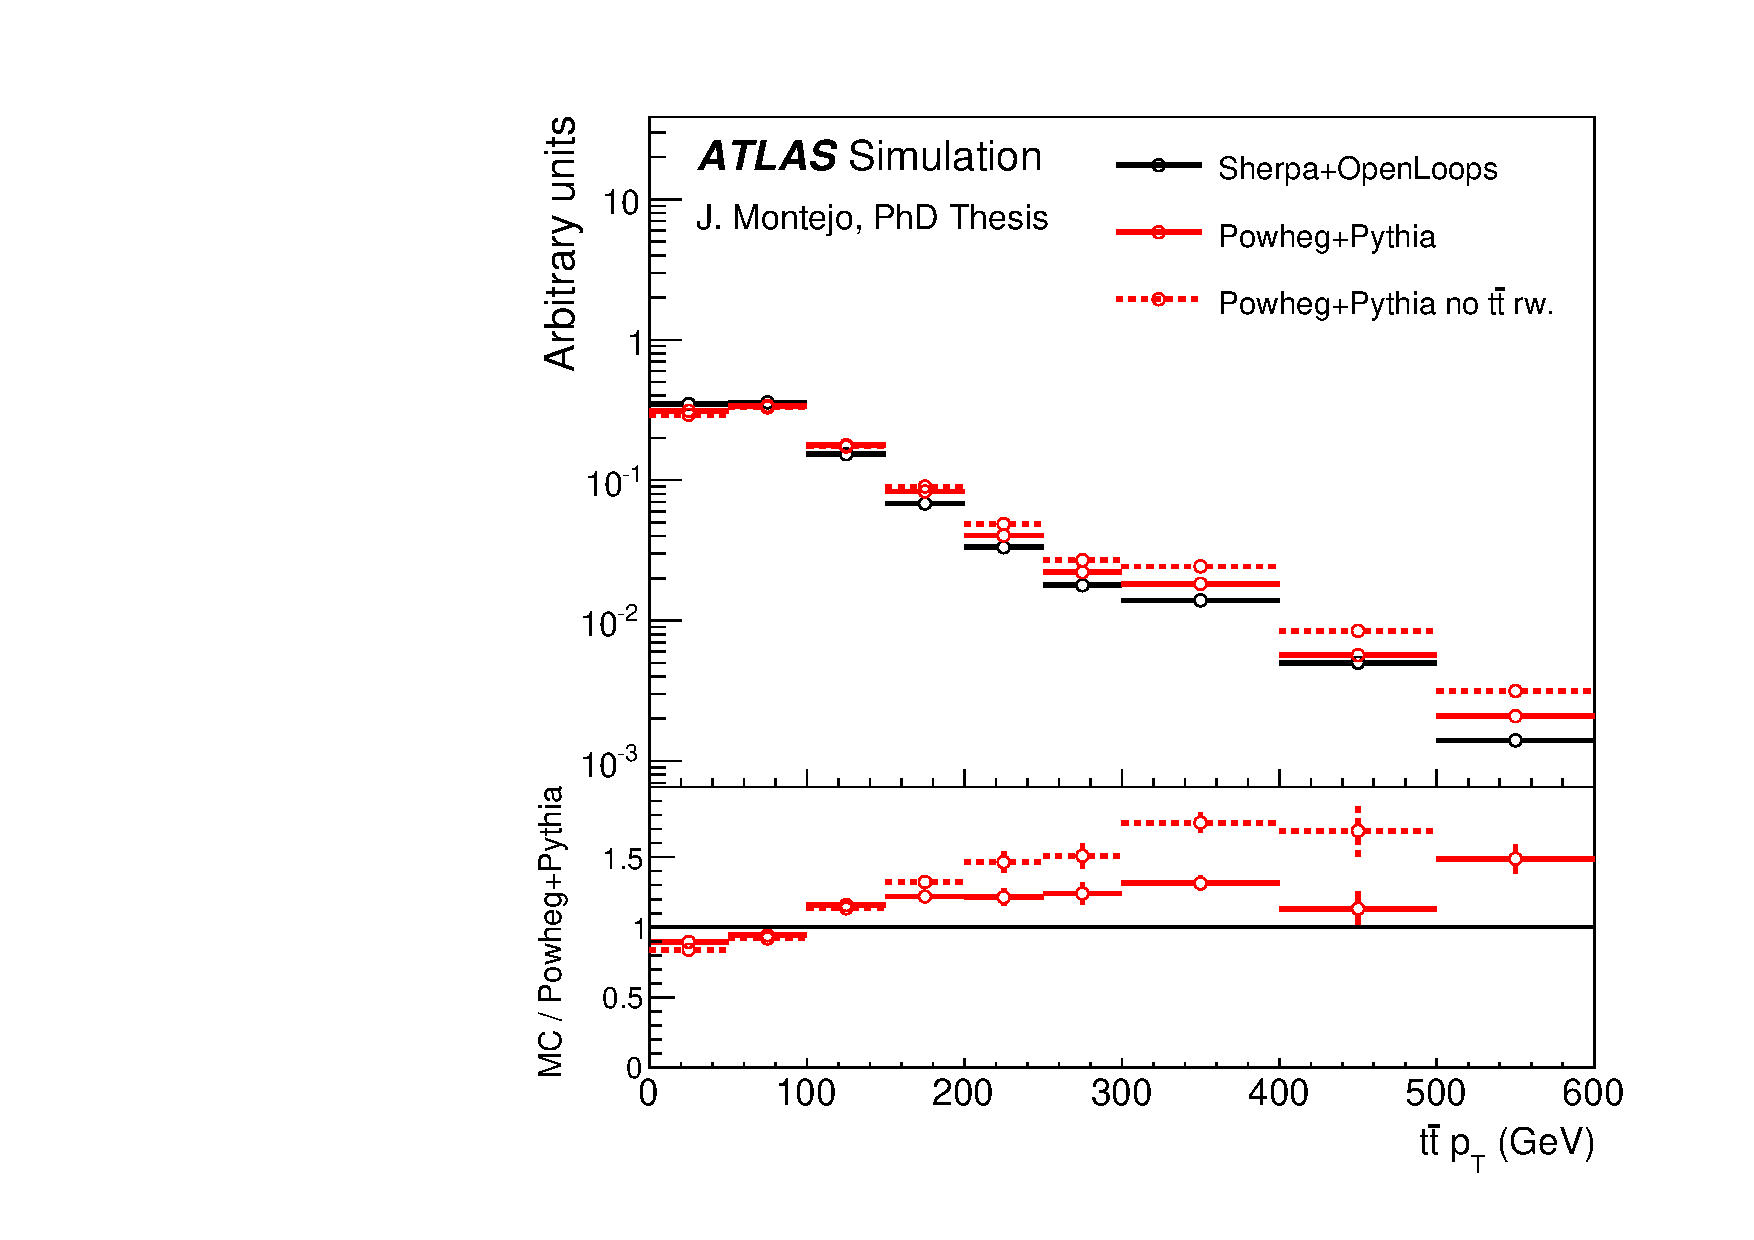
\includegraphics[width=0.46\textwidth]{Modeling/Figures/norw_tt1bq_ttbar_pt_norm}
  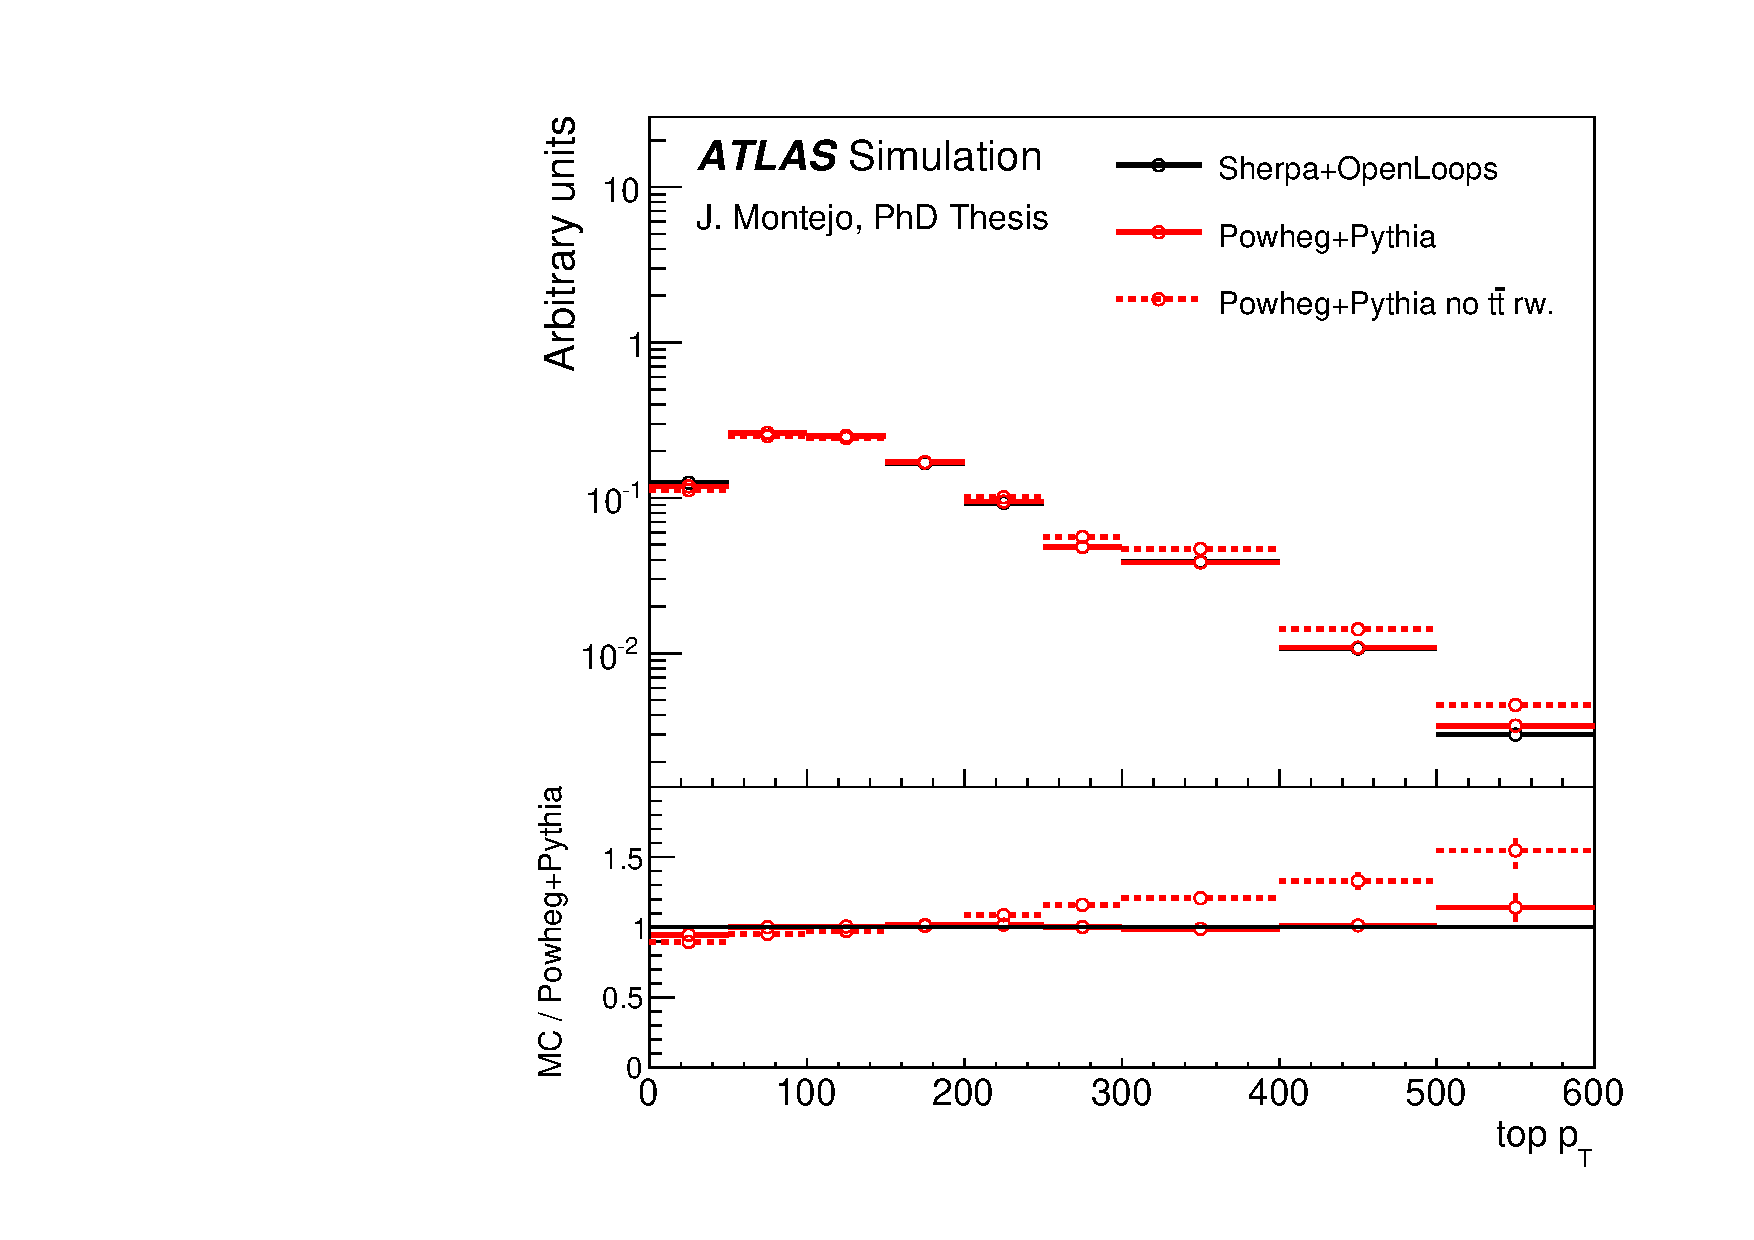
\includegraphics[width=0.46\textwidth]{Modeling/Figures/norw_tt1gbbq_top_pt_norm}
  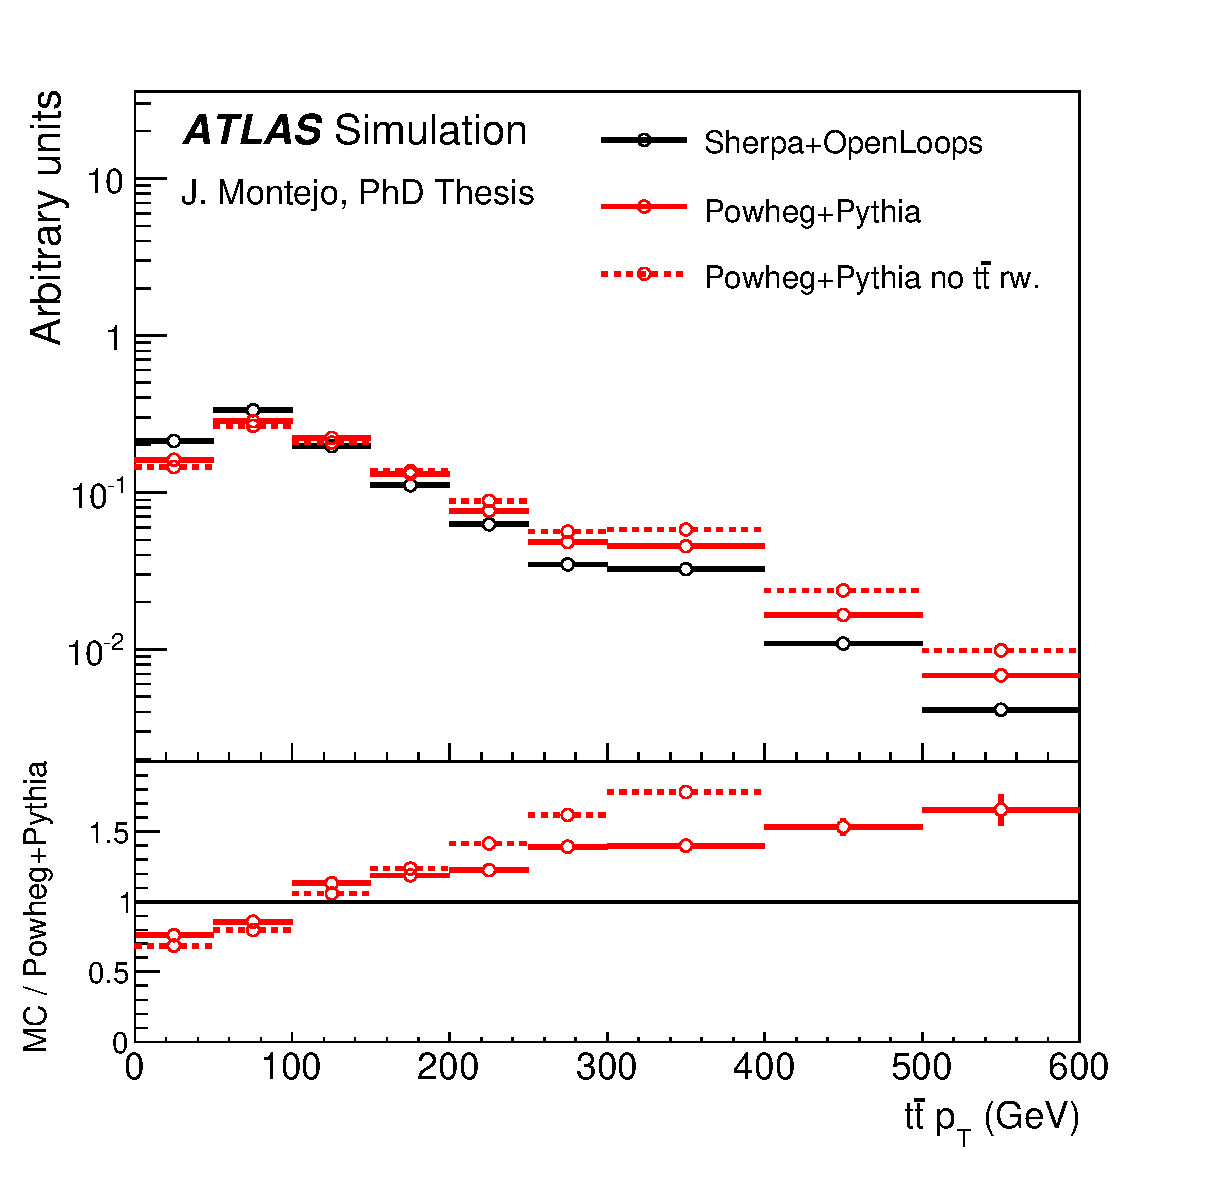
\includegraphics[width=0.46\textwidth]{Modeling/Figures/norw_tt1gbbq_ttbar_pt_norm}
  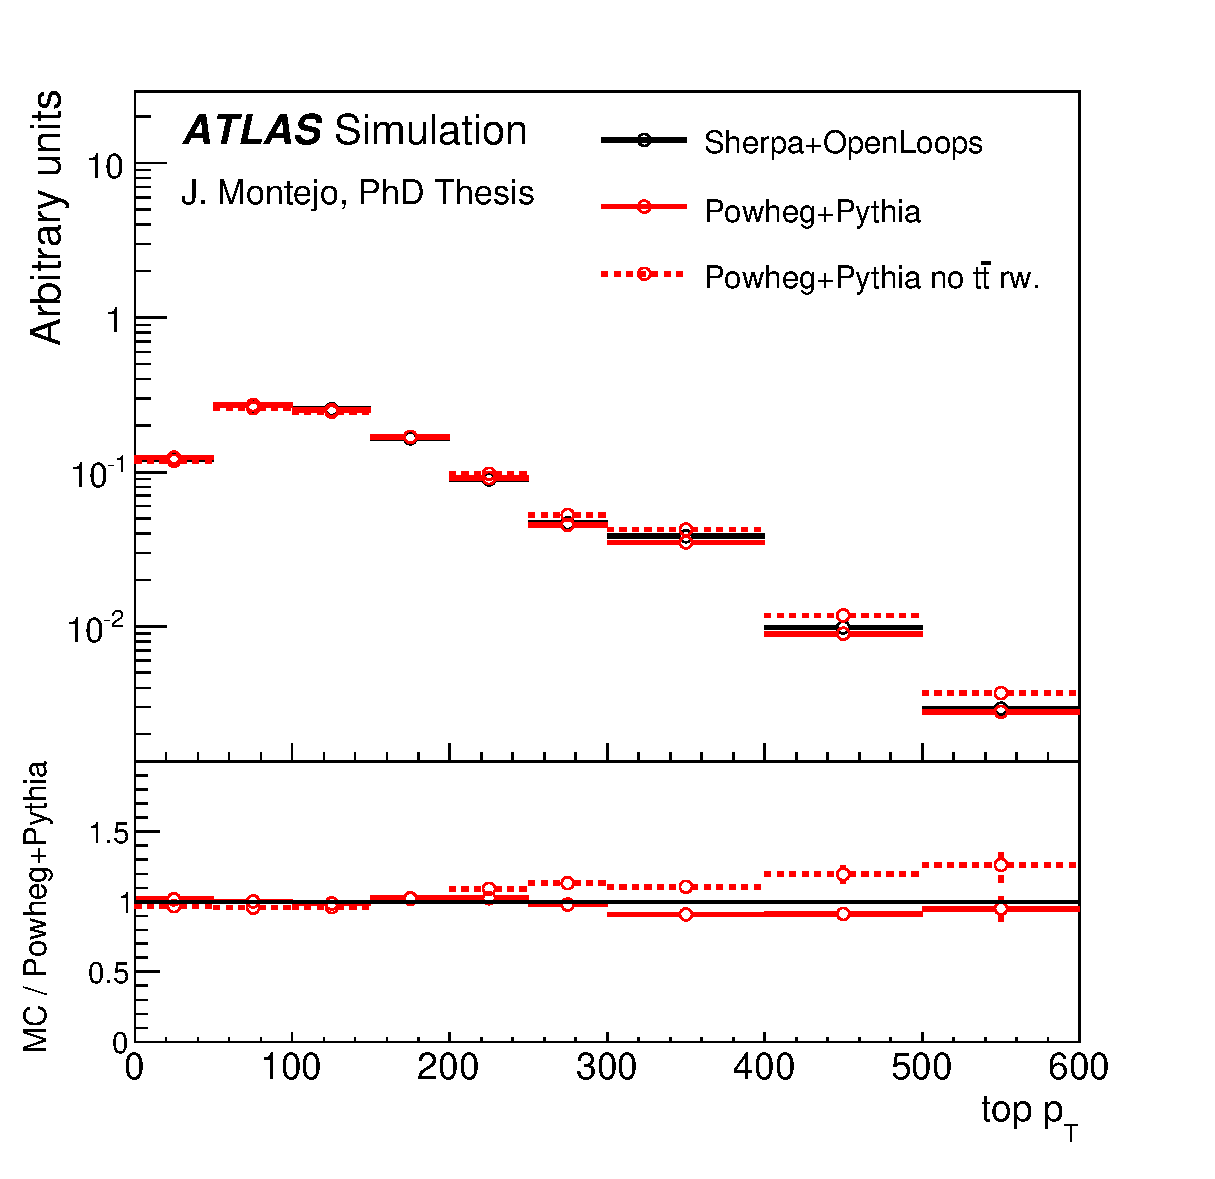
\includegraphics[width=0.46\textwidth]{Modeling/Figures/norw_tt2bq_top_pt_norm}
  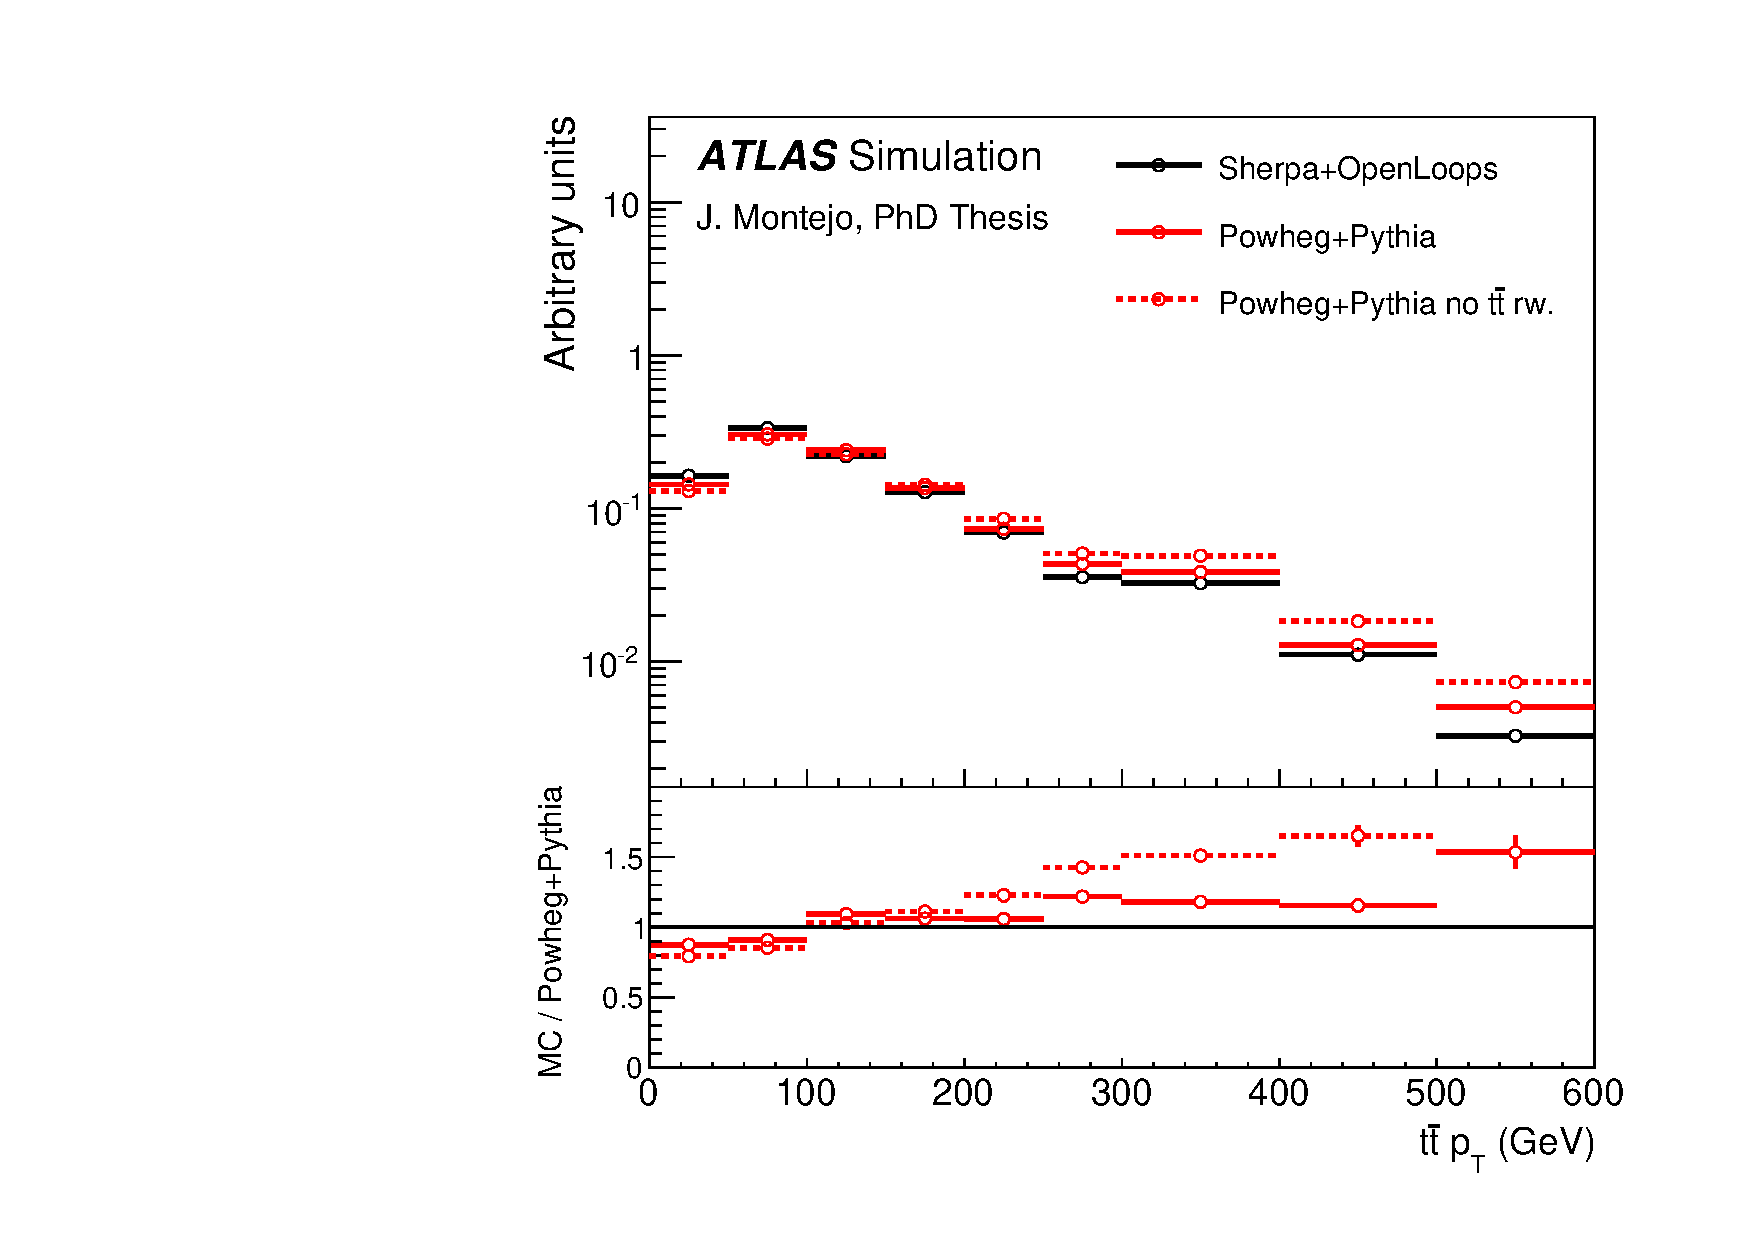
\includegraphics[width=0.46\textwidth]{Modeling/Figures/norw_tt2bq_ttbar_pt_norm}
\caption{
  Effect of the \ttbar\ reweighting derived from the differential \xsec\ measurement on the \ttbb\ sample. 
  The NLO prediction from \ShOL\ (black) is compared to \PP\ with (red solid) and without (red dashed) the \ttbar\ reweighting. The top quark \pt\ (left) and the transverse momentum of the \ttbar\ system (right) are compared in the different topologies: \ttb\ (upper row), \ttB\ (middle row) and \ttbb\ (bottom row).
}
\label{fig:ttreweighting_ttbb}
\end{center}
\end{figure}

Given the differences observed between the predictions of \PP\ and \ShOL, a reweighting procedure is 
implemented to improve the modeling.
The inclusive \ttbb\ \xsec\ is kept constant throughout all the reweightings, but the 
relative \xsec\ in each category is adjusted to the NLO prediction. 
Furthermore, two independent kinematic reweightings are
derived to improve the agreement of the different variables in each category.  
The first reweighting is based on the \pt\ of the top and \ttbar\ systems.
The second reweighting is chosen to be on the \pt\ and
\eta\ of the heavy-flavor jet in the topologies with only one additional heavy-flavor jet. 
In the topologies with
two or more heavy-flavor jets the reweighting is based on the $\Delta R$ and \pt\ of the 
dijet system. This
reweighting improves the modeling of the rest of the variables, though some minor 
differences remain.
The effect of the reweighting on different example variables is illustrated  in 
figure~\ref{fig:default_reweighting}. The full set of figures can be found in appendix~\ref{app:ttbb_modeling}.
\begin{figure}[tp]
\begin{center}
\begin{tabular}{cc}
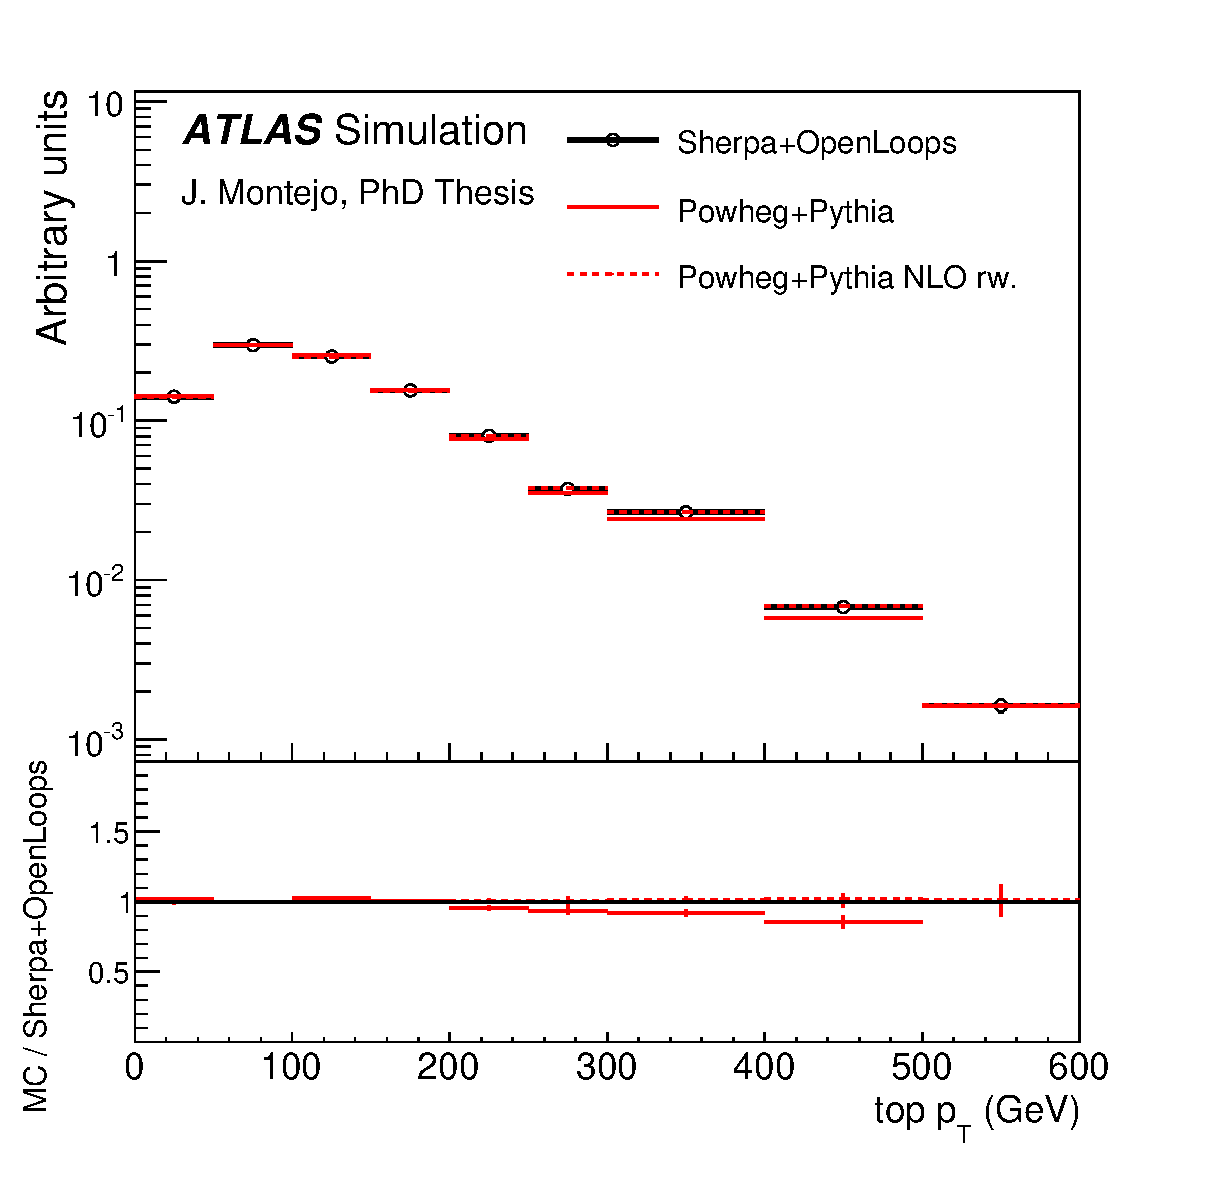
\includegraphics[width=0.48\textwidth]{Modeling/Figures/rw_tt1bq_top_pt.eps} &
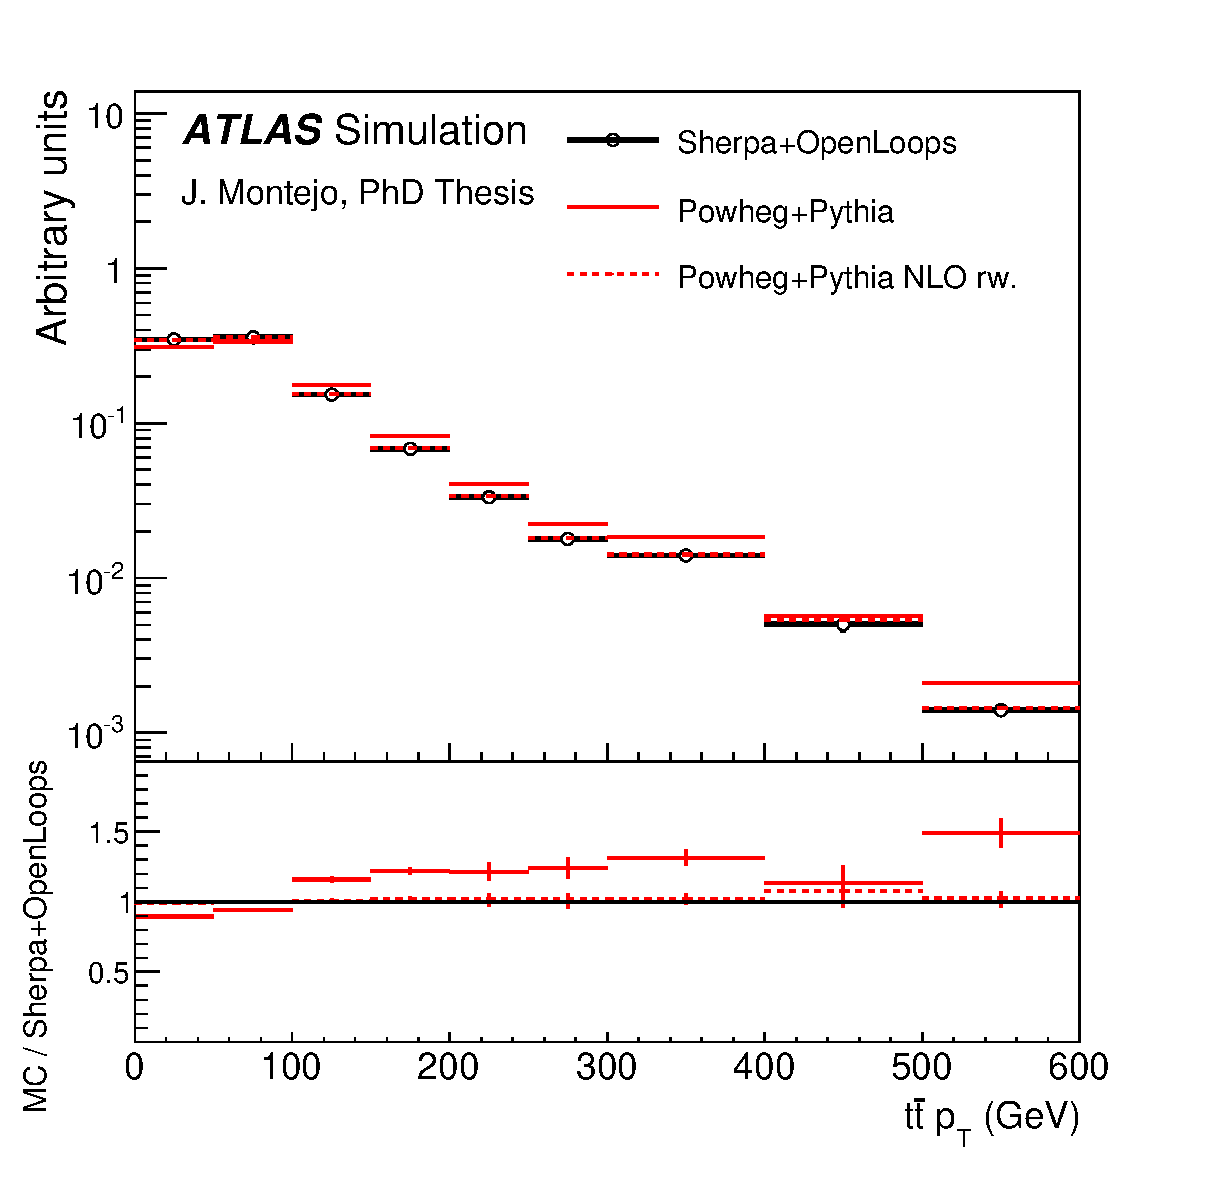
\includegraphics[width=0.48\textwidth]{Modeling/Figures/rw_tt1bq_ttbar_pt.eps} \\
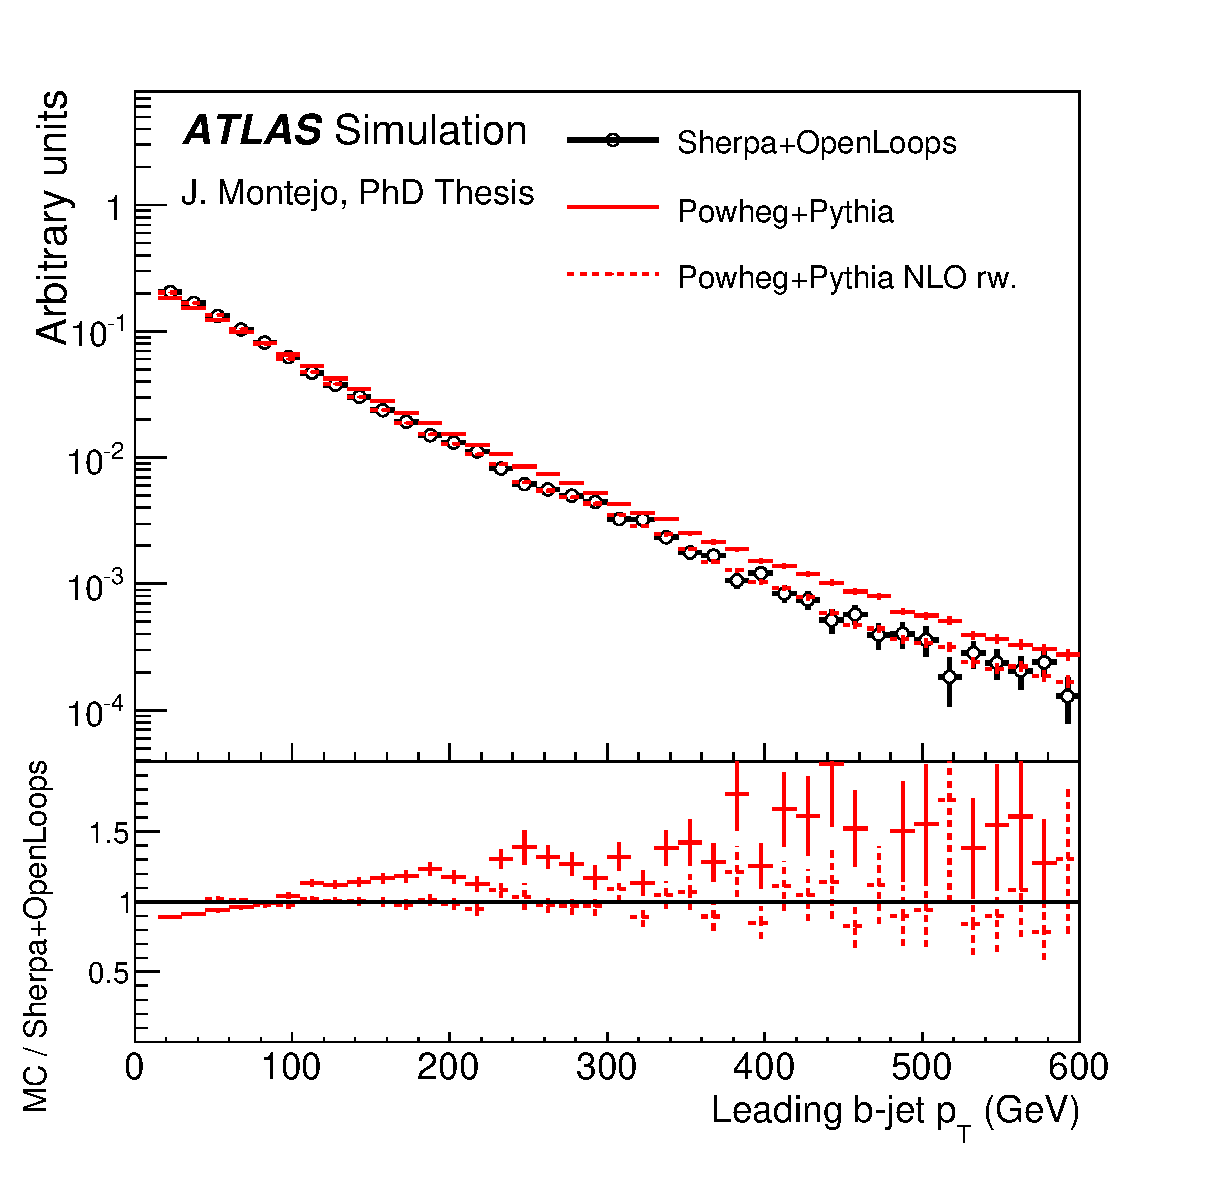
\includegraphics[width=0.48\textwidth]{Modeling/Figures/rw_tt1gbbq_q1_pt.eps} &
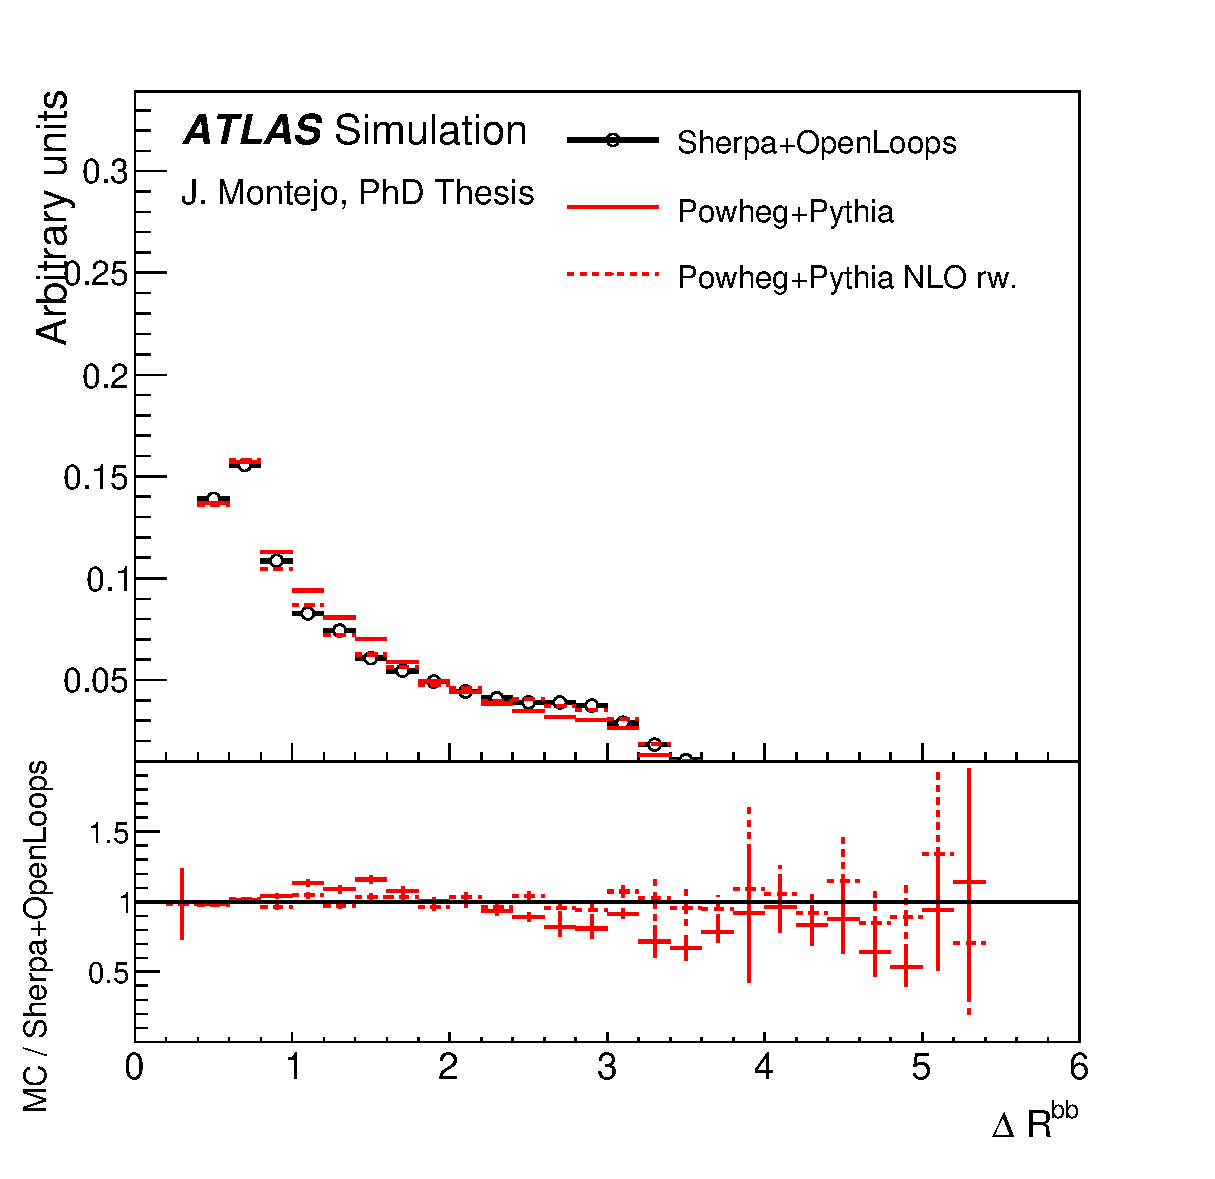
\includegraphics[width=0.48\textwidth]{Modeling/Figures/rw_ttbb_qq_dr.eps} \\
\end{tabular}
\caption{
  Effect of the \ttbar\ reweighting derived from the differential \xsec\ measurement on the \ttbb\ sample. 
  The NLO prediction from \ShOL\ (black) is compared to \PP\ with (red solid) and without (red dashed) the \ttbar\ reweighting. 
The different kinematic variables and topologies are: 
  \toppt\ in \ttb\ (top left), \ttbarpt\ in \ttb\ (top right), leading $b$-jet \pt\ in \ttB\ (bottom left) and $\DR^{\bbbar}$ in \ttbb\ (bottom right).}
\label{fig:default_reweighting}
\end{center}
\end{figure}

%\clearpage %latex runs out of memory without this, maybe just my laptop
 
\subsubsection{\texorpdfstring{\ttcc\ modeling}{ttcc modeling}}
\label{subsec:ttcc}
Unfortunately, no NLO calculations are available for the \ttcc\ background. Therefore the \ttcc\ prediction 
from \powheg\ is taken without any additional calibration, apart from the \ttbar\ reweighting.
The \ttcc\ modeling in \PP\ is validated by comparing to the multi-leg LO prediction in \madgraph.
Reasonable agreement between both generators can be seen in figure~\ref{fig:defaultcc_extHFtype} and 
a selection of kinematic variables is shown in figure~\ref{fig:defaultcc_example}. The full set of figures can be found in appendix~\ref{app:ttcc_modeling}.

A large difference is observed in the prediction of the MPI categories, which are modeled by the parton shower. Small differences in the settings of \pythia\ are present between both samples: \powheg\ uses \pythia\ 6.426, {\sc CTEQ61L} pdf and Sandhoff color-reconnection scheme~\cite{Buttar:2006zd}; whereas \madgraph\ uses \pythia\ 6.427, {\sc CT10} pdf and Wicke color-reconnection scheme~\cite{Skands:2007zg}. This difference will be covered by the systematic uncertainties on \ttcc\ modeling discussed in section~\ref{subsubsec:ttcc_syst}.

\begin{figure}[!t]
\begin{center}
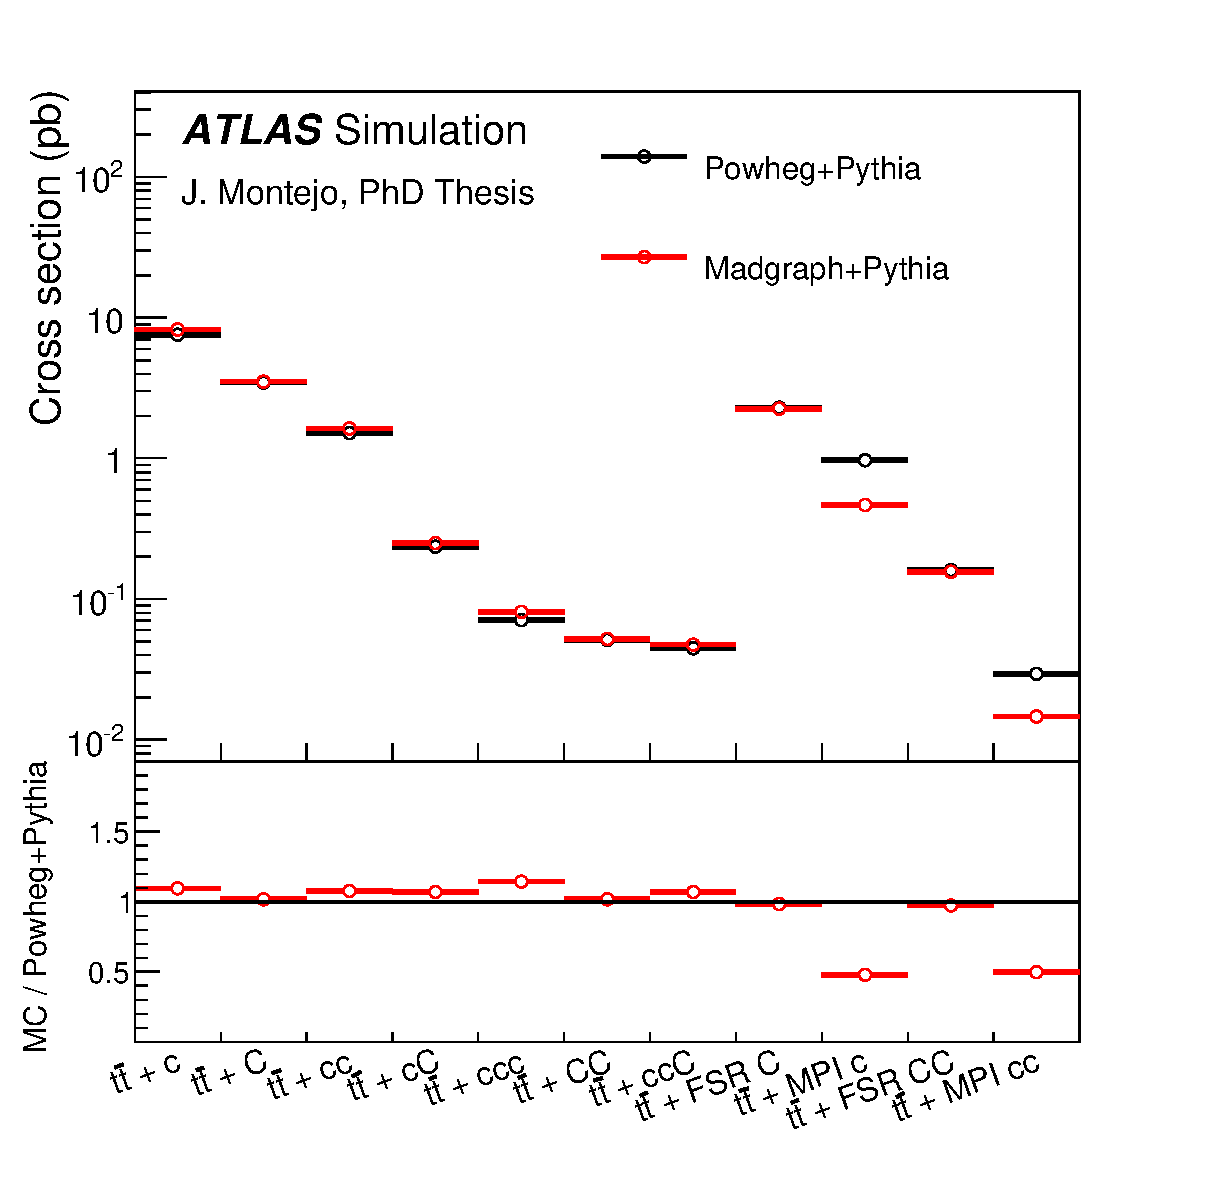
\includegraphics[width=0.7\textwidth]{Modeling/Figures/defaultcc_realHFcc_extHFtype_ttcc}
\caption{Comparison of \ttcc\ subcategories between \PP\ and \madgraph+\pythia.}
\label{fig:defaultcc_extHFtype}
\end{center}
\end{figure}

\begin{figure}[tp!]
\begin{center}
\begin{tabular}{cc}
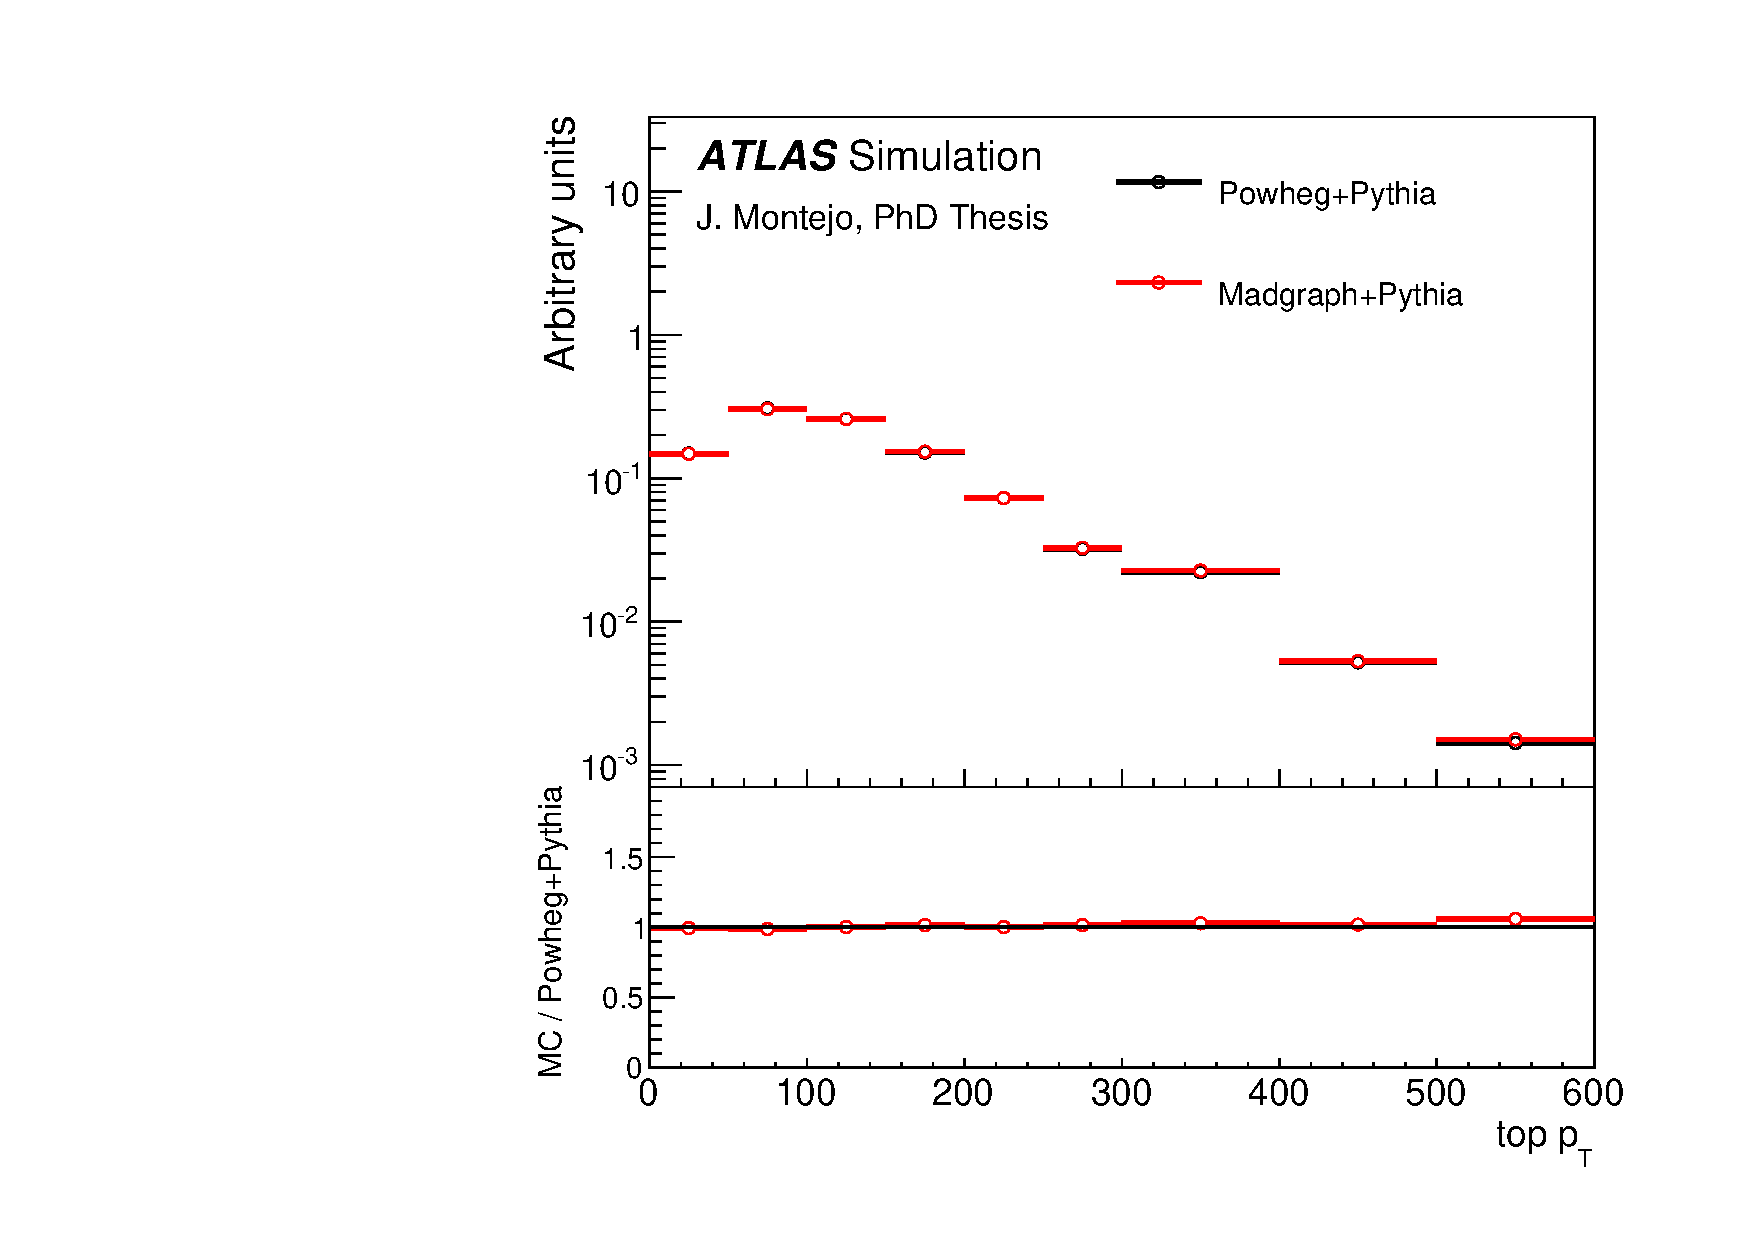
\includegraphics[width=0.48\textwidth]{Modeling/Figures/defaultcc_tt1cq_top_pt_norm} &
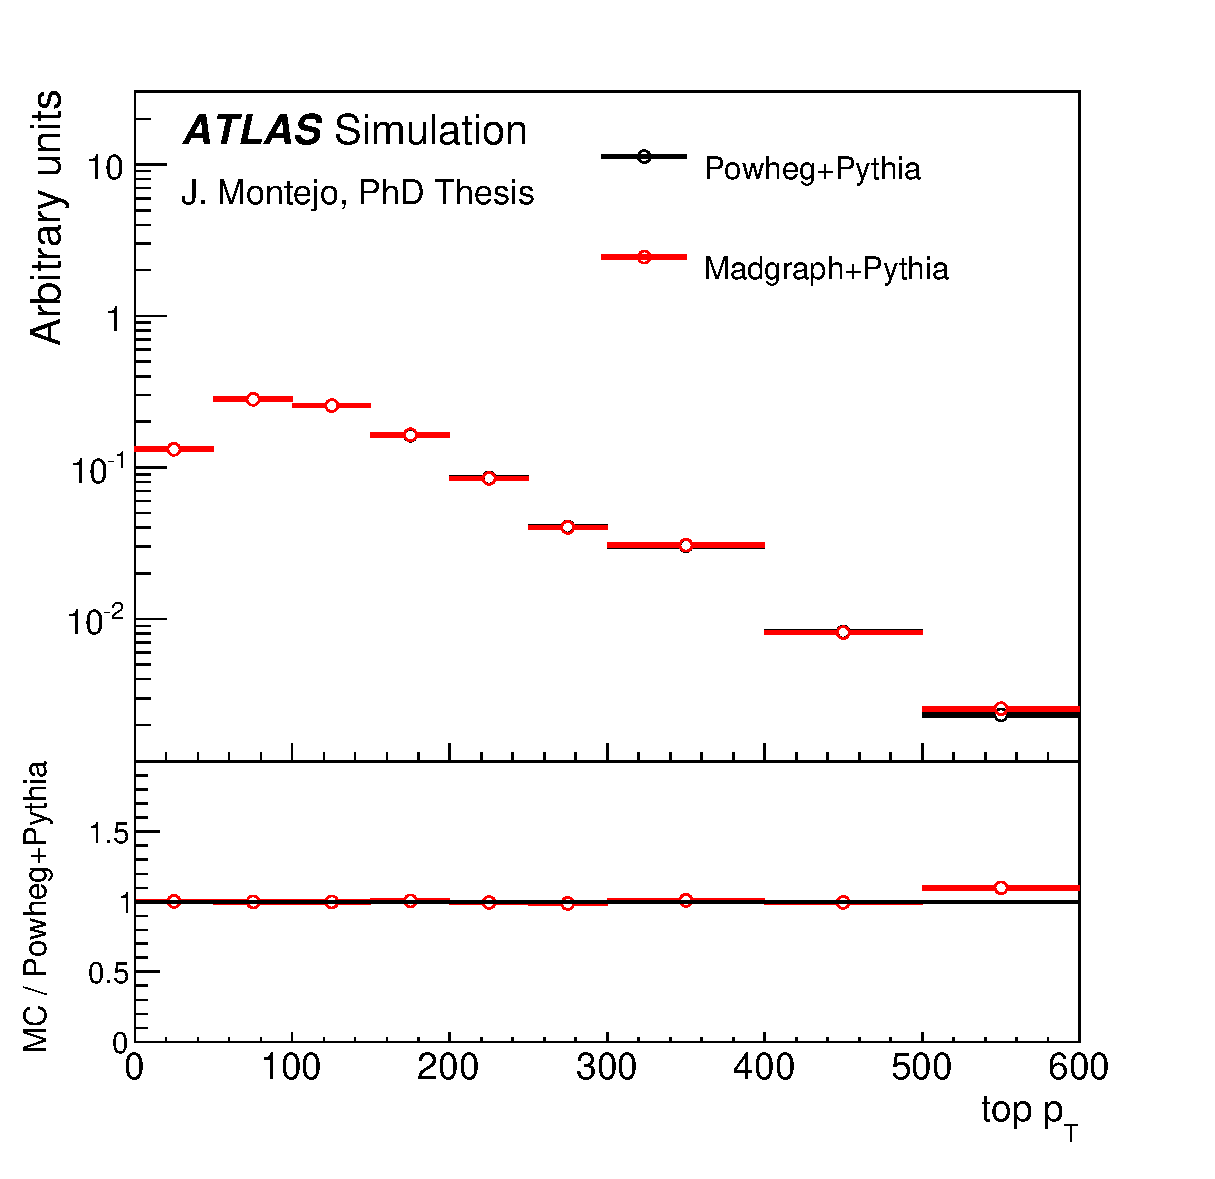
\includegraphics[width=0.48\textwidth]{Modeling/Figures/defaultcc_tt1gccq_top_pt_norm} \\
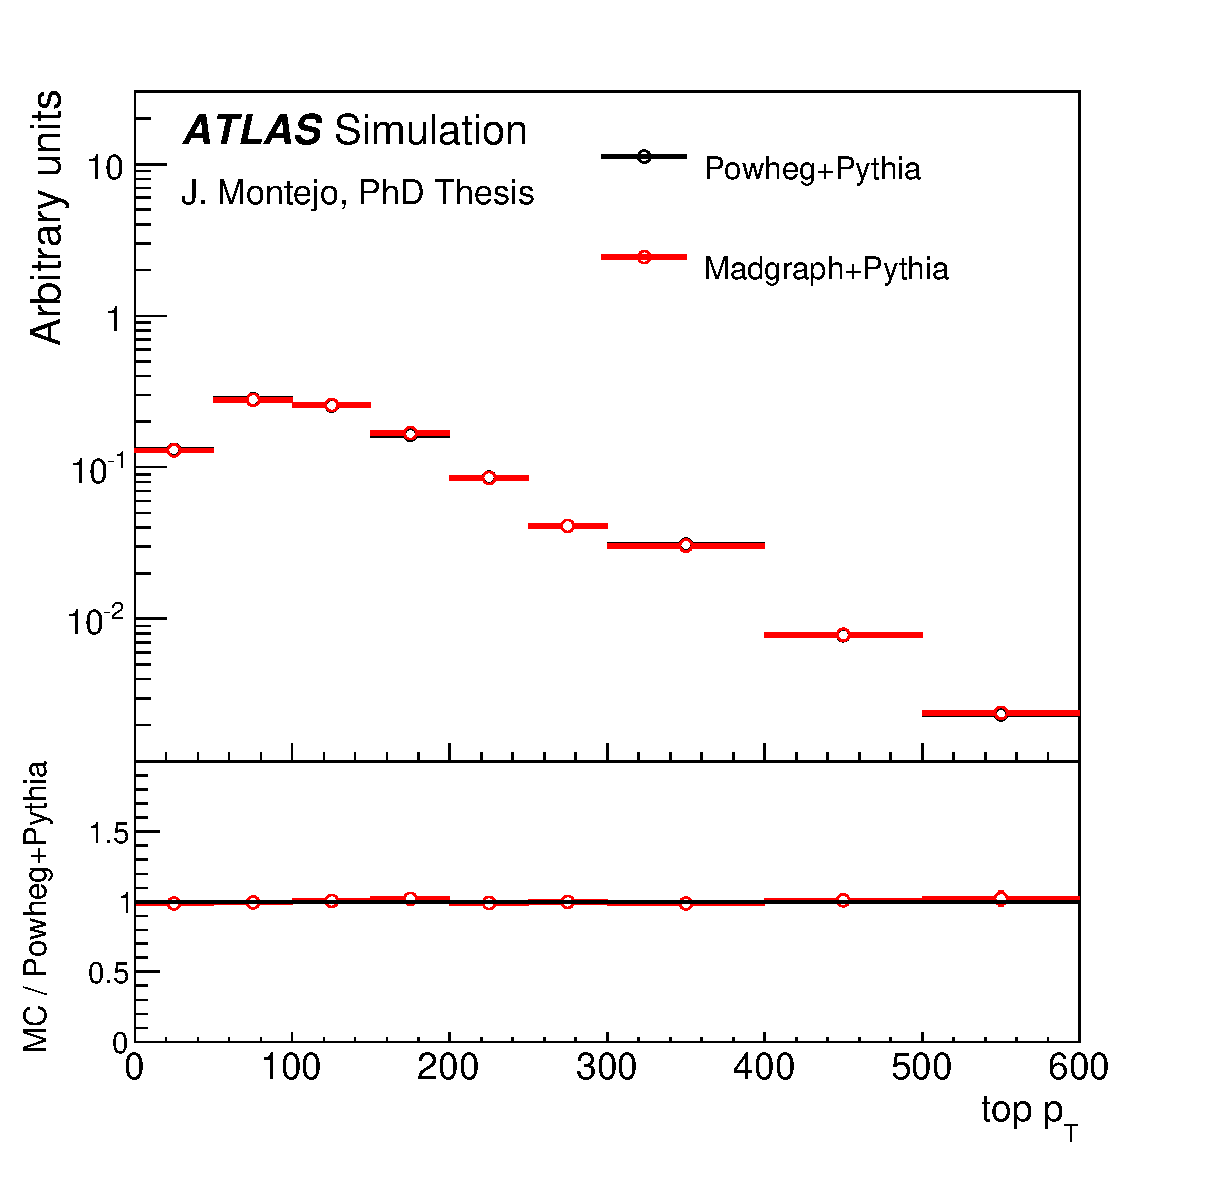
\includegraphics[width=0.48\textwidth]{Modeling/Figures/defaultcc_tt2cq_top_pt_norm} &
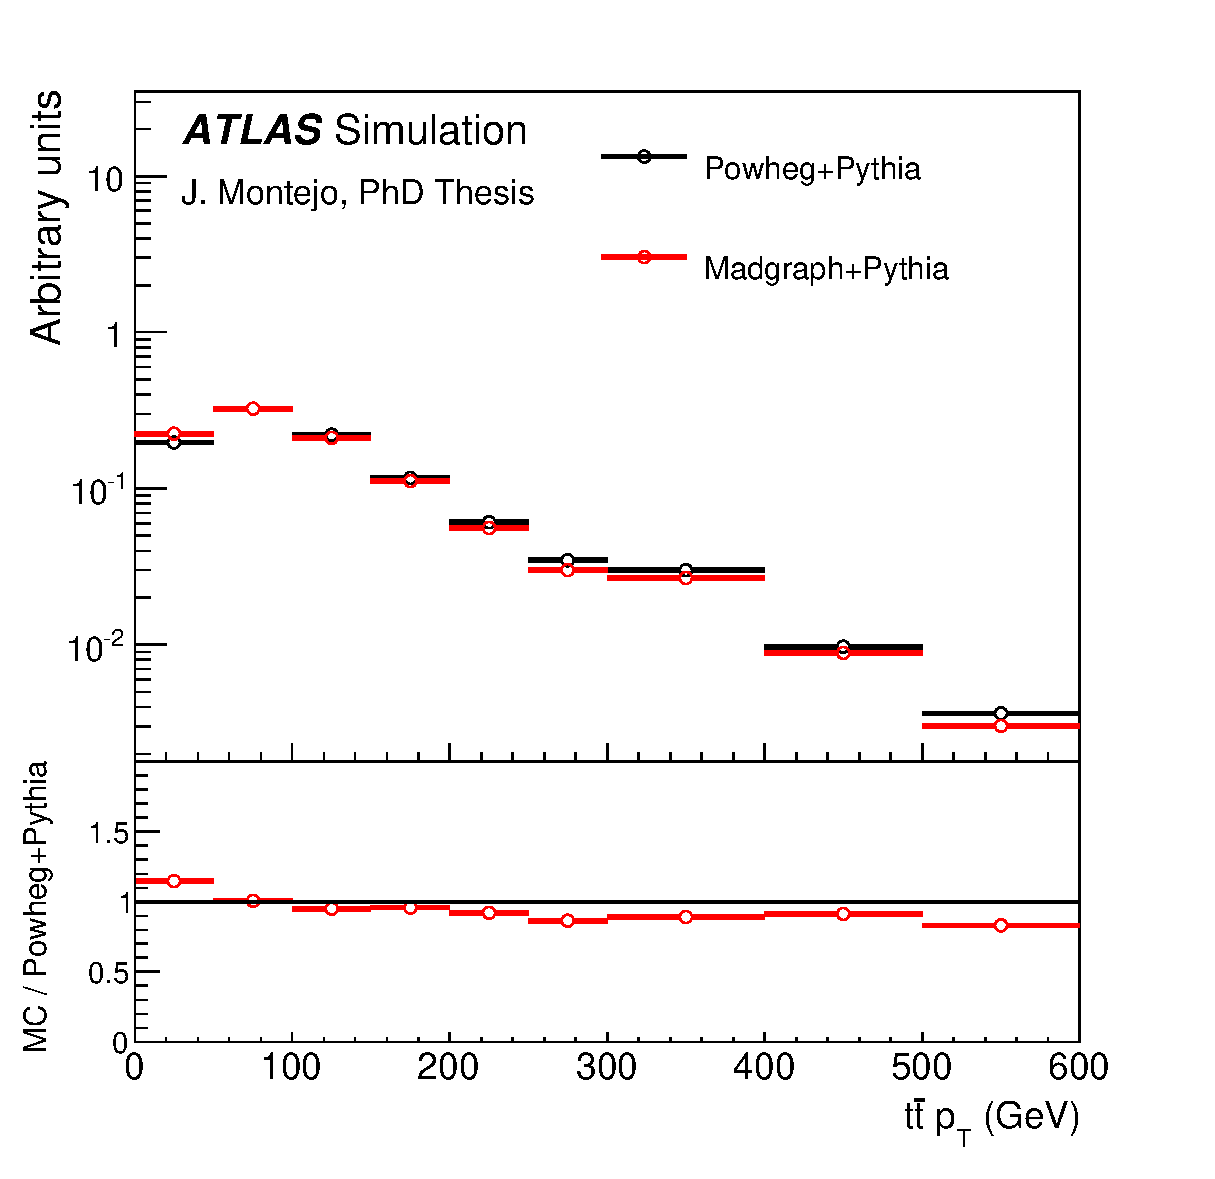
\includegraphics[width=0.48\textwidth]{Modeling/Figures/defaultcc_tt2cq_ttbar_pt_norm} \\
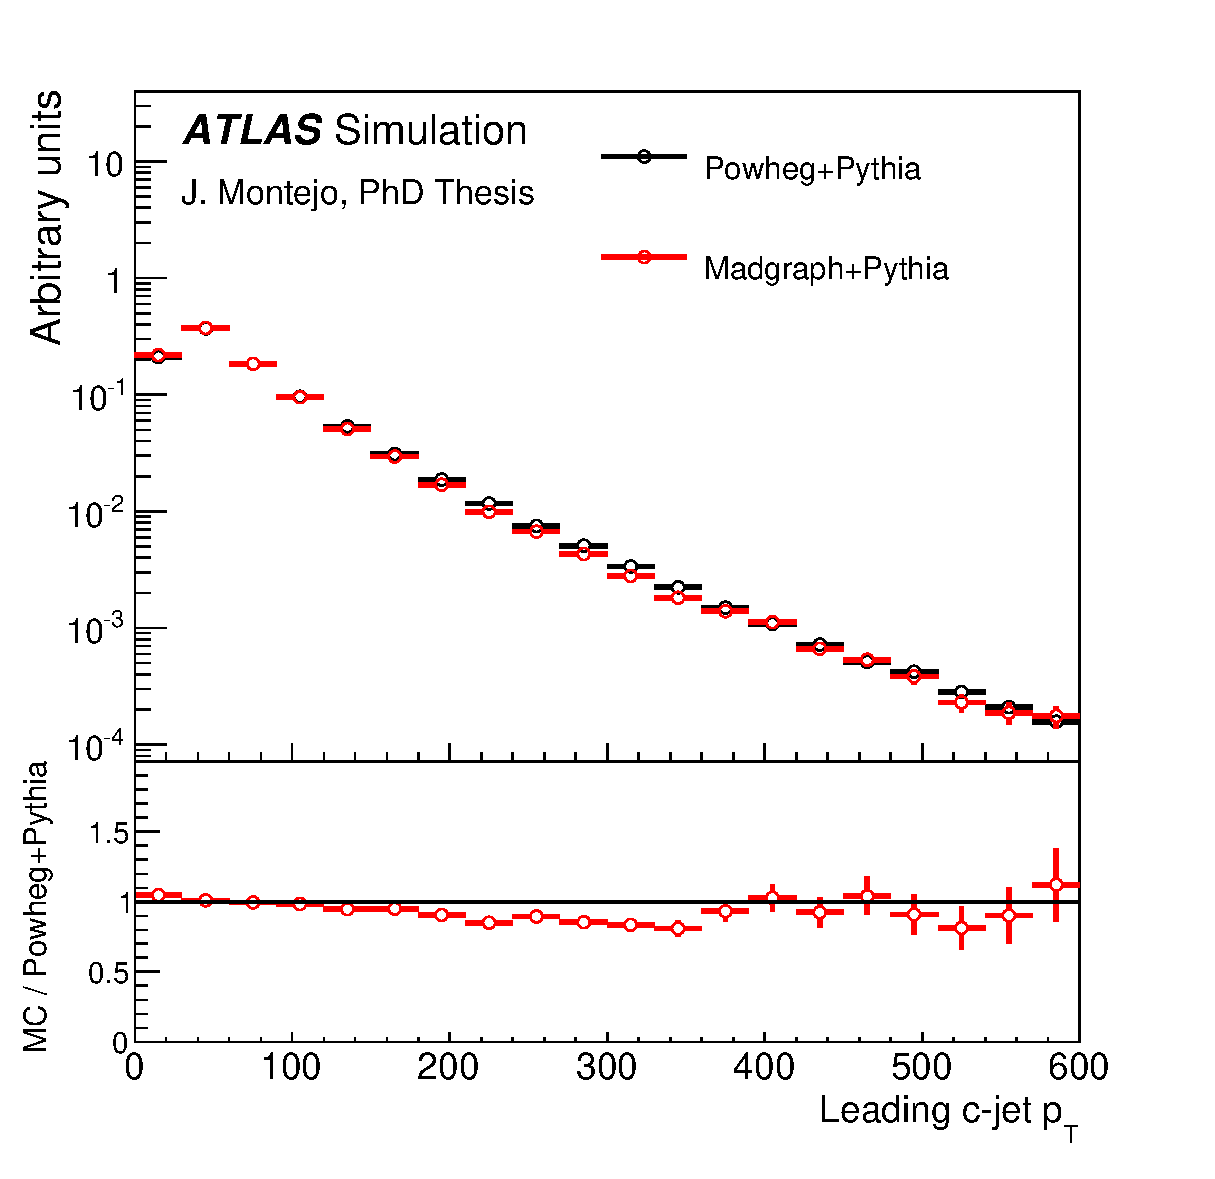
\includegraphics[width=0.48\textwidth]{Modeling/Figures/defaultcc_tt2cq_q1_pt_norm} &
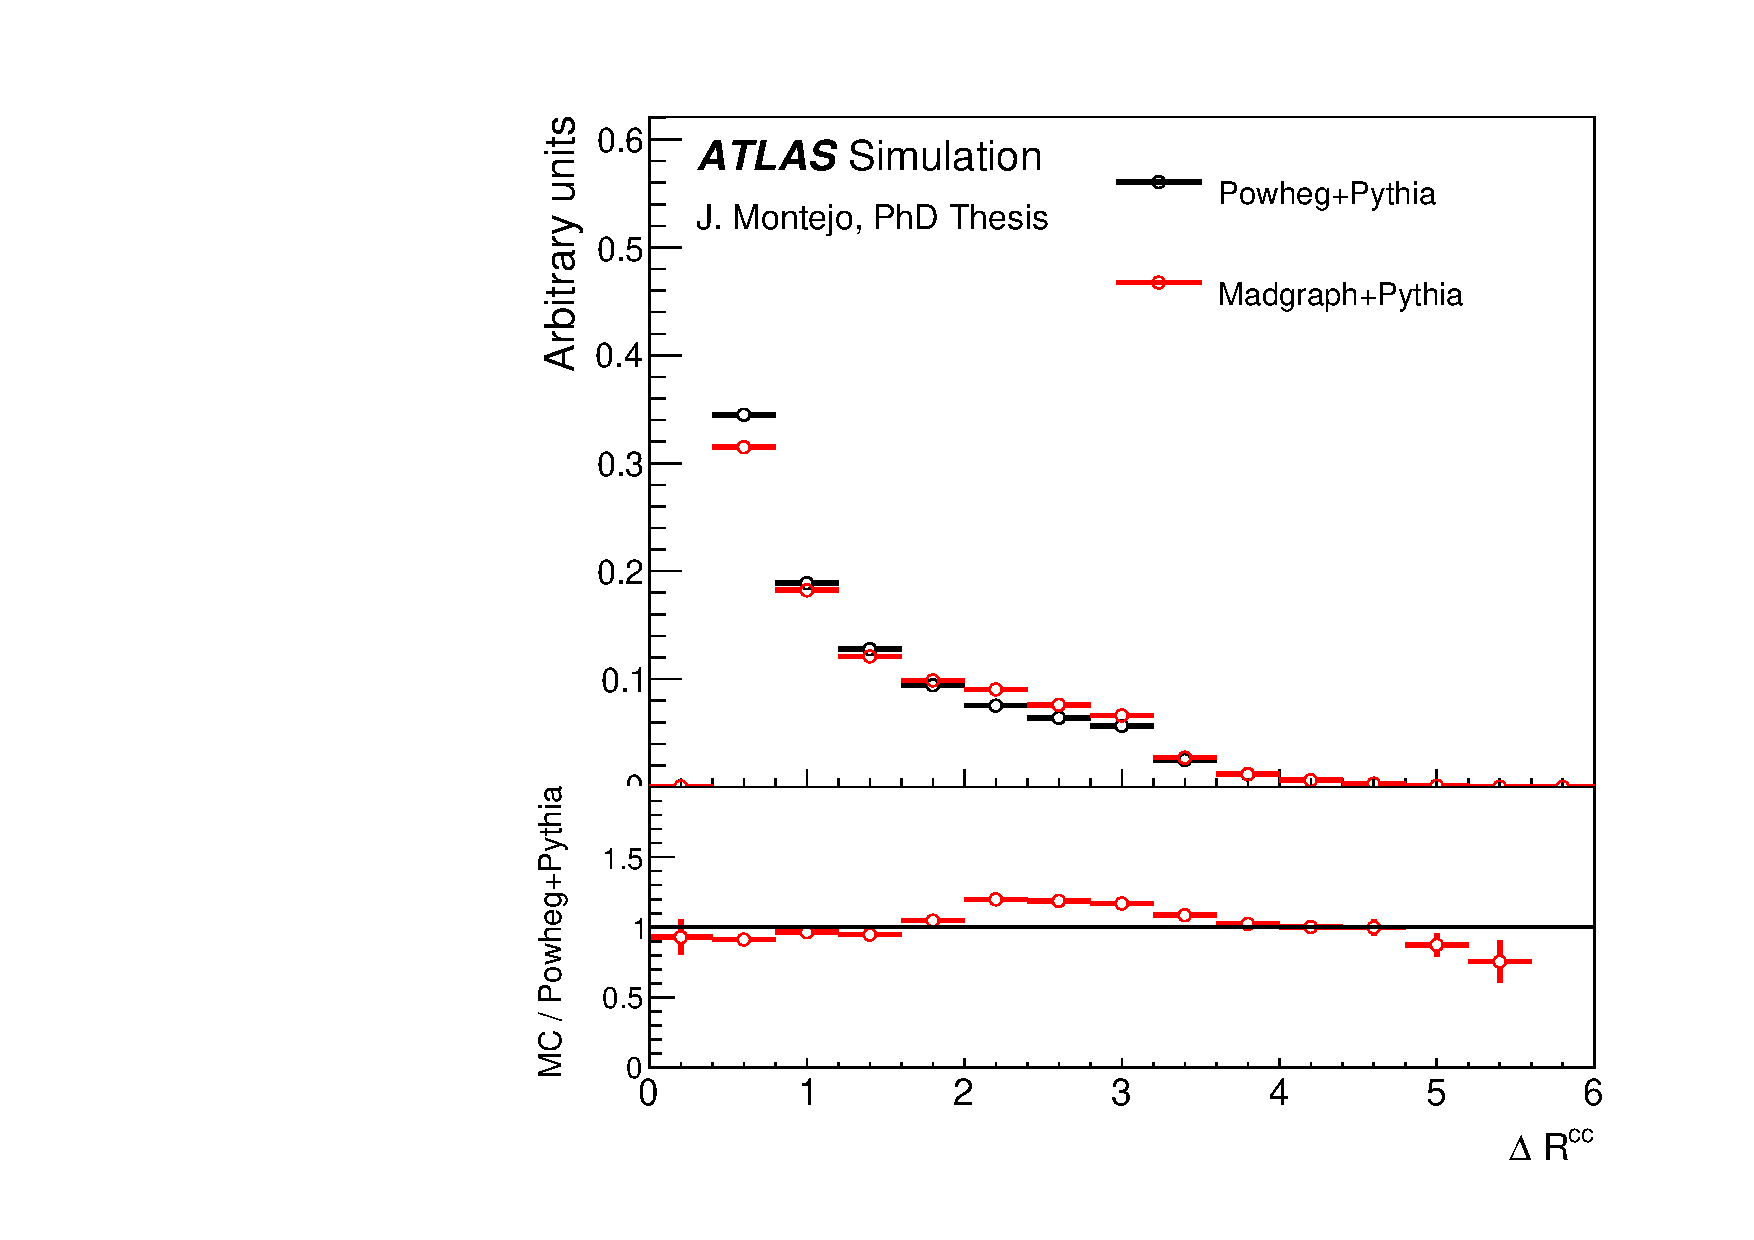
\includegraphics[width=0.48\textwidth]{Modeling/Figures/defaultcc_tt2cq_qq_dr_norm} \\
\end{tabular}
\caption{Comparison of kinematic variables in different topologies: \toppt\ in \ttc\ (top left), \toppt\ in \ttB\ (top right), \toppt\ in \ttcc\ (middle left), \ttbarpt\ in \ttcc\ (middle right), leading $c$-jet \pt\ in \ttcc\ (bottom left) and $\DR^{\ccbar}$ in \ttcc\ (bottom right).}
\label{fig:defaultcc_example}
\end{center}
\end{figure}


\subsection{$W/Z$+jets background}
The background contribution from the production of a vector boson, $V=W,Z$, with additional jets is simulated 
with \alpgen\ 2.14~\cite{alpgen} and the
{\sc CTEQ6L1} PDF set. Parton shower and fragmentation are modeled with \pythia\ 6.425.

Both samples are generated with up to five
additional partons, separately for $V$+light-jets,
$Vb\bar{b}$+jets, $Vc\bar{c}$+jets, and in the case of $W$ production, also $Wc$+jets.
Both are normalized to the respective inclusive NNLO theoretical \xsecs~\cite{vjetsxs}.
The overlap between $V+Q\bar{Q}$ ($Q=b,c$)
events generated from the matrix element calculation and those
from parton-shower evolution in the $V$+light-jet  
samples is removed by an algorithm based on the angular separation
between the extra heavy quarks: if $\Delta R(Q,\bar{Q})>0.4$, the
matrix element prediction is used, otherwise the parton shower
prediction is used. 

In the measurement of the differential \xsec\ of the $Z$ \pt\ spectrum~\cite{Zjetsxsec}, \alpgen\ has been observed to predict a too hard spectrum.
The MC has been reweighted to correct for this effect. 
The heavy-flavor fraction of the $Z$+jets background, i.e. the sum of 
$Z$+\bbbar\ and $Z$+\ccbar\ processes, is scaled by a factor of 1.52 in order to
reproduce the relative rates of $Z$ events with no $b$-tags and those with at least one $b$-tag observed in data.

Given the similarity in the generation setup of the $W$+jets and $Z$+jets backgrounds, the corrections derived in the $Z$+jets sample are also applied to $W$+jets. 

\subsection{Other simulated backgrounds}
Backgrounds with small \xsecs\ or low acceptance are also considered for completeness. Although some of them could be considered negligible, especially in the signal regions, their absence in the control regions could affect the result of the fit, which would propagate to the signal region. %Crap, I haven't discussed the fit yet.

Samples of single top quark production, corresponding to the
$s$-channel, $t$-channel and $Wt$ production mechanisms are generated with 
\powheg\ using the {\sc
CT10} PDF set.  In the case of the $Wt$-channel, the diagram removal scheme is 
used to handle the overlap with the \ttbar\ final state starting at NLO~\cite{mcatnlo_3}.
The samples are interfaced 
to {\sc Pythia} 6.425 with the {\sc CTEQ6L1} set of parton 
distribution functions and Perugia2011C underlying-event tune.  
The single top quark samples are normalized to
the approximate NNLO theoretical \xsecs~\cite{stopxs,stopxs_2,stopxs_3}
using the {\sc MSTW2008} NNLO PDF set~\cite{mstw1,mstw2}. 
The small contribution from single top production in association with a $Z$ boson is simulated
with \madgraphfive\ and \pythia 8.1~\cite{PythiaManual8}, and normalized to its LO prediction.

Samples of diboson production in association with up to three jets are generated with \alpgen\ 2.14 and showered with \herwig\ 6.520. They are further normalized to the NLO theoretical \xsecs~\cite{dibosonxs}.

Samples of $t\bar{t}+V$ with up to two jets are generated with \madgraphfive\ and 
the {\sc CTEQ6L1} PDF set. 
{\sc Pythia} 6.425 with the AUET2B tune~\cite{ATLASUETune1,ATLASUETune2} is used for showering. 
The $t\bar{t}+V$ samples are normalized to the NLO \xsec\ predictions~\cite{ttbarVxs1,ttbarVxs2}.
Production of $t\bar{t}+WW$ is also taken into account, being simulated with \madgraphfive\ and showered with \pythia 8.1.

The $t\bar{t}+Z$ background, with subsequent $Z\rightarrow\bbbar$, is an irreducible background and has very similar kinematics to the \ttH\ signal. Despite having a larger \xsec, $\unit[205]{fb}$ compared to $\unit[129]{fb}$, the significantly smaller branching ratio of $Z\rightarrow\bbbar$, \unit[15]{\%}, reduces its contribution to less than half of the \ttHbb\ signal.


\subsection{Multijet background}
\label{subsec:QCD}
Multijet events can enter the selected data sample through several
production and mis-reconstruction mechanisms. 
In the electron  
channel, the multijet background consists of non-prompt electrons from heavy-hadron decays,
and ``fake'' electrons arising from
photon conversions and mis-identified jets with a high fraction of
their energy deposited in the EM calorimeter.  
In the muon channel,
the background contributed by multijet events is predominantly due to
final states with non-prompt muons, such as those from semileptonic $b$-
or $c$-hadron decays. 

While the probability of reconstructing a lepton from a ``fake'' source in a multijet event is very low, the production \xsec\ for multijet events is orders of magnitude above \ttbar\ production. 
Since this background is very difficult to model accurately with a MC simulation, a data-driven method referred to as \textit{Matrix Method}~\cite{TOPFAKES8TeV} (MM) is used to estimate the expected number of multijet events in the final selection sample.
The MM exploits the differences
in lepton properties between prompt, isolated
leptons from $W$ and $Z$ boson decays, referred to as ``real leptons'',
and those where the leptons are either non-isolated or result
from the mis-identification of photons or jets, called ``fake leptons''. 
Two samples are defined after imposing the final kinematic selection
criteria, differing only in the lepton identification criteria: a
``tight'' sample and a ``loose'' sample, the former being a subset of
the latter.  The tight selection applies the lepton
identification criteria used in the analysis. 
For the loose selection some of the lepton identification or isolation requirements are omitted, as defined in section~\ref{sec:Leptons}.  
The number of selected events in each sample ($\nl$ and $\nt$)
can be expressed as a linear combination of the numbers of events with
real and fake leptons, in such a way that the following system of
equations can be defined:
\begin{eqnarray}
\nl &=& \nlr + \nlf, \nonumber \\
\nt &=&  \epsr \nlr +  \epsf \nlf,
\label{eq:MM}
\end{eqnarray}
\noindent where $\epsr$ ($\epsf$) represents the probability for a real (fake) lepton satisfying
the loose criteria to also satisfy the tight one, and both are measured
in data control samples. 
The contribution of fake leptons in the tight sample can be obtained as:
\begin{equation}
  \ntf = \frac{\epsf}{\epsr - \epsf}(\epsr \nl - \nt)
  \label{eq:ntf}
\end{equation}

The following conditions must be satisfied for the method to work with reasonable precision:
\begin{itemize}
  \item The loose sample should have an efficiency that is sufficiently different numerically, so that the statistical precision of the mis-identified background estimation is not compromised by the term $1/(\epsr -\epsf)$.
  \item The efficiencies are assumed to be independent from the event topology, so that they can be determined in control samples and be applied to the analysis sample. E.g. \epsr\ must be similar for leptons originating from $W$+jets, $Z$+jets, and \ttbar.
  \item Any significant dependence of the efficiencies on the kinematics or topology must be parameterized in order to obtain an accurate modeling.
\end{itemize}

The real efficiency \epsr\ is measured using the tag-and-probe method from $\Zee$ and $\Zmumu$ control regions. 
The average $\epsr$ is $\sim$0.75 ($\sim$0.98) in the
electron (muon) channel. 

To measure $\epsf$, samples enriched in multijet background are selected
by requiring either low $\met$ and \mtw\ in the electron channel, or high impact parameter significance for the lepton track in the muon channel.
The average $\epsf$ value is $\sim$0.15 in both channels. 

Dependencies 
of $\epsr$ and $\epsf$ on quantities such as lepton $\pt$ and $\eta$, $\Delta R$ between the
lepton and the closest jet, or number of $b$-tagged jets, are parameterized in order to obtain
a more accurate estimate. 

\subsection{Signal modeling}
Signal samples are modeled using MC simulation. An accurate signal prediction is needed in order to asses the expected performance of the analyses and test the compatibility of a possible excess in data with a given hypothesis. 

\subsubsection{\texorpdfstring{\ttH\ signal}{ttH signal}}
The \ttH\ signal process is modeled at NLO accuracy
using matrix elements obtained from the HELAC-Oneloop package~\cite{Helac}.
In this case \powheg\ serves as an interface to
shower MC programs. The samples created using this approach are referred 
to as {\sc PowHel} samples~\cite{Garzelli:2011vp}. The \ttH\ sample is produced using 
the {\sc CT10}nlo PDF set~\cite{Lai:2010vv} and 
factorization ($\mu_{\rm F}$) and renormalization ($\mu_{\rm R}$) scales are set to
$\mu_{\rm F} = \mu_{\rm R} = \mt+\mH/2$. 
Showering is performed with {\sc Pythia} 8.1 using the CTEQ6L1 PDF set and the AU2 UE tune.
Inclusive decays for the Higgs boson are assumed in the generation of the $\ttH$ sample.
The $\ttH$ sample is normalized using the NLO \xsec~\cite{Dawson:2003zu,Beenakker:2002nc,Beenakker:2001rj}  
and the Higgs decay branching ratios~\cite{Djouadi:1997yw,Bredenstein:2006rh,Actis:2008ts,Denner:2011mq} collected in reference~\cite{Dittmaier:2011ti}.

\subsubsection{Vector-like quark signal}
For vector-like quarks signals, samples corresponding to a singlet $\T$ quark 
decaying to $Wb$, $Zt$ and $Ht$, and a singlet $\B$ quark decaying to $Wt$, $Zb$ and $Hb$ are generated with the {\sc Protos} v2.2 LO generator~\cite{jaas,protos} 
using the  {\sc MSTW2008} LO PDF set, and interfaced to {\sc Pythia} 6.426 for the parton shower and fragmentation. 
For each decay channel of the vector-like quark the branching ratio has been set to 1/3. Events are then reweighted
in order to reproduce any desired branching ratio configuration. 

The vector-like quark mass values considered range from $350\gev$ to $1100\gev$ in steps of $50\gev$.
All Higgs boson decay modes are considered, with branching ratios predicted at NNLO~\cite{Dittmaier:2011ti}.
Events are filtered at the generator level to require at least one lepton ($e$, $\mu$, or $\tau$) with $\pt>\unit[10]{\gev}$ and $|\eta|<2.8$. 
Signal samples are normalized to the theoretical calculation performed at next-to-next-to-leading order (NNLO) in QCD  
that includes resummation of next-to-next-to-leading-logarithmic (NNLL) soft-gluon terms 
with {\sc top++2.0}, with the same input choices as for \ttbar\ production.

\subsubsection{\texorpdfstring{$\stoptwo\bar{\st}_2$ signal}{t2t2 signal}}
Samples of $\st_2\bar{\st}_2$ and $\st_1\bar{\st}_1$ signal are generated with {\sc Herwig++} v2.5.2~\cite{herwigpp} with the {\sc CTEQ6L1} PDF set and UEEE3 UE tune~\cite{Gieseke:2012ft}. 
Signal samples are normalized using \xsecs\ calculated at NLO+NLL accuracy~\cite{Beenakker:1997ut,Beenakker:2010nq,Beenakker:2011fu}. 
Samples for $\st_2\bar{\st}_2$ production are generated for several configurations of $(m_{\st_2}, m_{\neut})$ 
keeping the mass relation between $\st_1$ and $\neut$ fixed to $m_{\st_1}=m_{\neut}+180\gev$. 
In the case of the $\st_2\bar{\st}_2$ samples,  $\st_2$ decays to $Z \st_1$, $H \st_1$ and $t \neut$ are considered.
In all samples the decay $\st_1 \to t \neut$  is assumed to have 100\% branching ratio, and
top quarks and the Higgs boson are decayed inclusively with SM branching ratios. 

Two sets of $\st_2\bar{\st}_2$ samples are generated. In the first set the $\st_2 \to H \st_1$ decay is forced assuming 100\% branching ratio
and a wide range of $(m_{\st_2}, m_{\neut})$ values is covered, up to $(m_{\st_2}=\unit[700]{\gev}, m_{\neut}=\unit[370]{\gev})$ in a two-dimensional grid with \unit[50]{\gev} steps. 
In the second set all three $\st_2$ 
decay modes ($Z \st_1$, $H \st_1$ and $t \neut$) are generated with branching ratio of 1/3 and only a few mass configurations
are available:  $(m_{\st_2}, m_{\neut}) = (350, 20)$, $(350, 70)$, $(500, 20)$, $(500, 70)$, $(700, 120)$, and $(700, 220)\gev$. 
At the analysis level $\st_2\bar{\st}_2$ events are reweighted in order to reproduce any desired branching ratio configuration.   

\subsubsection{Universal extra dimensions signal}
The generation of four-top events from the UED/RPP model is performed in two steps. 
First \madgraphfive\ is used to generate pairs of tier $(1,1)$ particles. In the second step, BRIDGE~\cite{Meade:2007js} is used
to chain-decay these particles down to the four-tops final state. Four mass points are considered:
$m_{\KK}$ = 600, 800, 1000 and \unit[1200]{\gev}. In all cases, the branching ratio of $A^{(1,1)} \to \ttbar$ and the ratio of
the two radii, $\xi = R_4/R_5$, are set to 1. The samples are normalized to the LO \xsecs\ as computed by \madgraph\ 
with the MSTW2008LO PDF set. %The \xsecs\ are summarized in table~\ref{tab:ued_xs}.

%\begin{table}[!t]
%\centering
%\begin{tabular}{ c c }
%\toprule
%\toprule
%\multicolumn{2}{c}{UED/RPP}  \\
%\midrule
%$m_{\KK}$ [\gev] & \Xsec\ [fb]\\
%\midrule
%600  & 1285 \\
%800  & 114 \\
%1000 & 11.7 \\
%1200 & 1.22 \\
%\bottomrule
%\bottomrule
%\end{tabular}
%\caption{
%\Xsecs\ for four top events from a UED/RPP model with different \KK\ masses.
%}
%\label{tab:ued_xs}
%\end{table}

\subsubsection{Sgluon signal}
Samples for sgluon pair production with different masses have been generated, $m_{\sigma}$ = 350, 400, 500, 600, 800, 1000 and \unit[1250]{\gev}.
All samples are generated using \pythia6 for the event level generation, parton showering and
hadronization, with the CTEQ6L1 PDF.
The samples are normalized to the NLO \xsec~\cite{GoncalvesNetto:2012nt}.

%http://arxiv.org/pdf/1203.6358v1.pdf

\subsubsection{Four-tops signal}
Four-top production with a contact interaction is generated with \madgraphfive\ and the MSTW2008LO PDF, setting the renormalization and factorization scales to $\mu_R = \mu_F = 4m_t$, where $m_t$ is the top quark mass.
The prescription of reference~\cite{Degrande:2010kt} is followed where the contact interaction is not directly implemented. 
Instead, a new heavy colorless vector particle
($\rho$) coupling to the right handed top is introduced. This model has two additional parameters: 
the coupling constant between the top quark and $\rho$ ($g_\rho$) and the mass of heavy mediator ($M_\rho$).
The latter is set to a very high value in order to be in the regime where the exchange of $\rho$ can be contracted to a contact interaction.
In this regime, the four-top production depends only on the ratio of the two parameters. Therefore there is a
unique free parameter: the contact interaction coupling constant $C_{4t}/\Lambda^2 = -g_\rho^2/(2M_\rho^2)$.

A choice for the values of $g_\rho$ and $M_\rho$ has to be made, providing that $M_\rho$ is sufficiently large to be in the contact
interaction regime. The values used in this analysis are: 
\begin{eqnarray*}
  g_\rho &=& 100 \sqrt{8\pi} \\
  M_\rho &=& 100 \tev
\end{eqnarray*}
which gives $C_{4t}/\Lambda^2 = -4\pi \tev^{-2}$. The LO production \xsec\ computed by \madgraph\ is \unit[42.2]{fb}. 
Only the \xsec\ depends on the chosen parameters while the event kinematics don't~\cite{Aliev:1482159}.

The SM production of four-top events has a very small \xsec\ ($\sigma_\fourtop \approx \unit[1]{fb}$ at $\sqrt{s} = 8 \tev$~\cite{Barger:2010uw}) 
and the interference between the SM and the new physics model described above has been
found to be negligible~\cite{Degrande:2010kt}.
Since the four top quarks process has never been observed, it is also
interesting to be able to set a limit on this process. A sample of SM four-top events is also generated with the same generator and scale described for the contact interaction.
%removing of course the non-Standard Model operators.

\section{Comparison between data and prediction}
In order to validate the good modeling of the main backgrounds by the simulation, a first set
of data/MC comparisons is presented at the preselection level.
The preselection requirement of at least two $b$-jets suppresses the non-\ttbar\ background, leaving a sample dominated by \ttbar+jets. 
Figures~\ref{fig:plots_1} and~\ref{fig:plots_2} show basic kinematic variables at the preselection level. Figure~\ref{fig:bjet_n_4j0b} shows the
$b$-tag multiplicity spectrum without the preselection requirement of at least two $b$-jets.

\begin{figure}[tp!]
  \centering
  \begin{subfigure}{0.32\textwidth}
  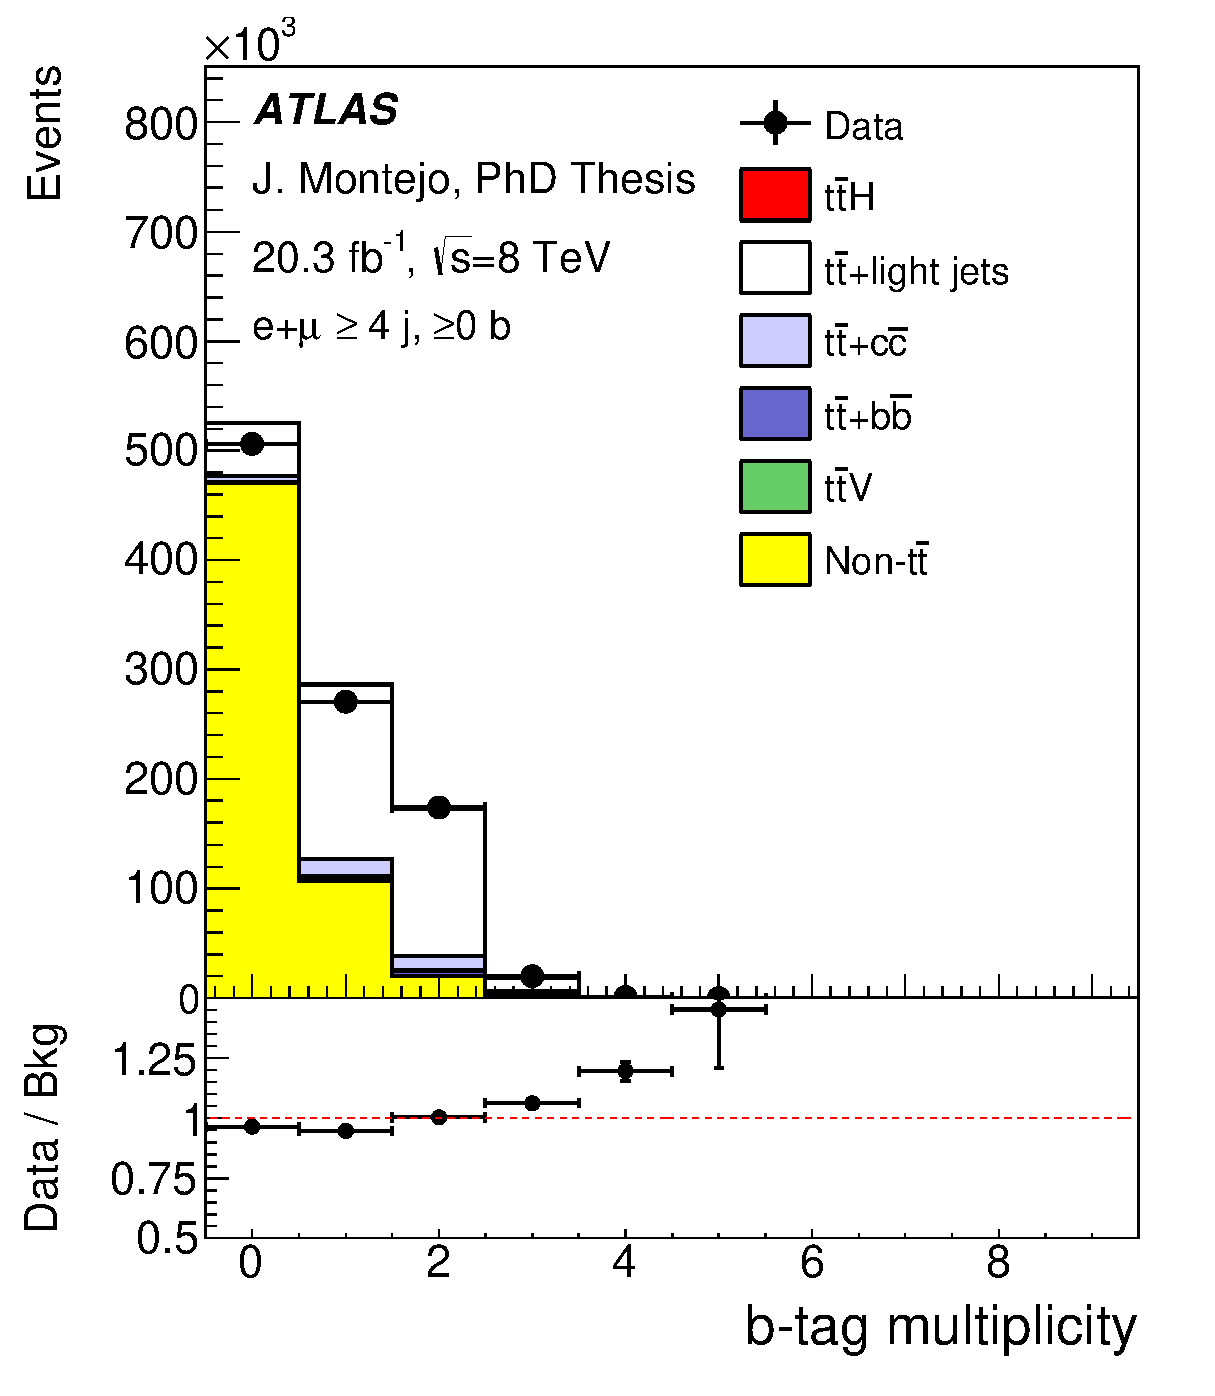
\includegraphics[width=\textwidth]{Modeling/Figures/plots_4j0b/bjet_n_ELEMUON_4jetin0btagin_NOMINAL.eps}
  \caption{}\label{fig:bjet_n_4j0b} \end{subfigure}
  \begin{subfigure}{0.32\textwidth}
  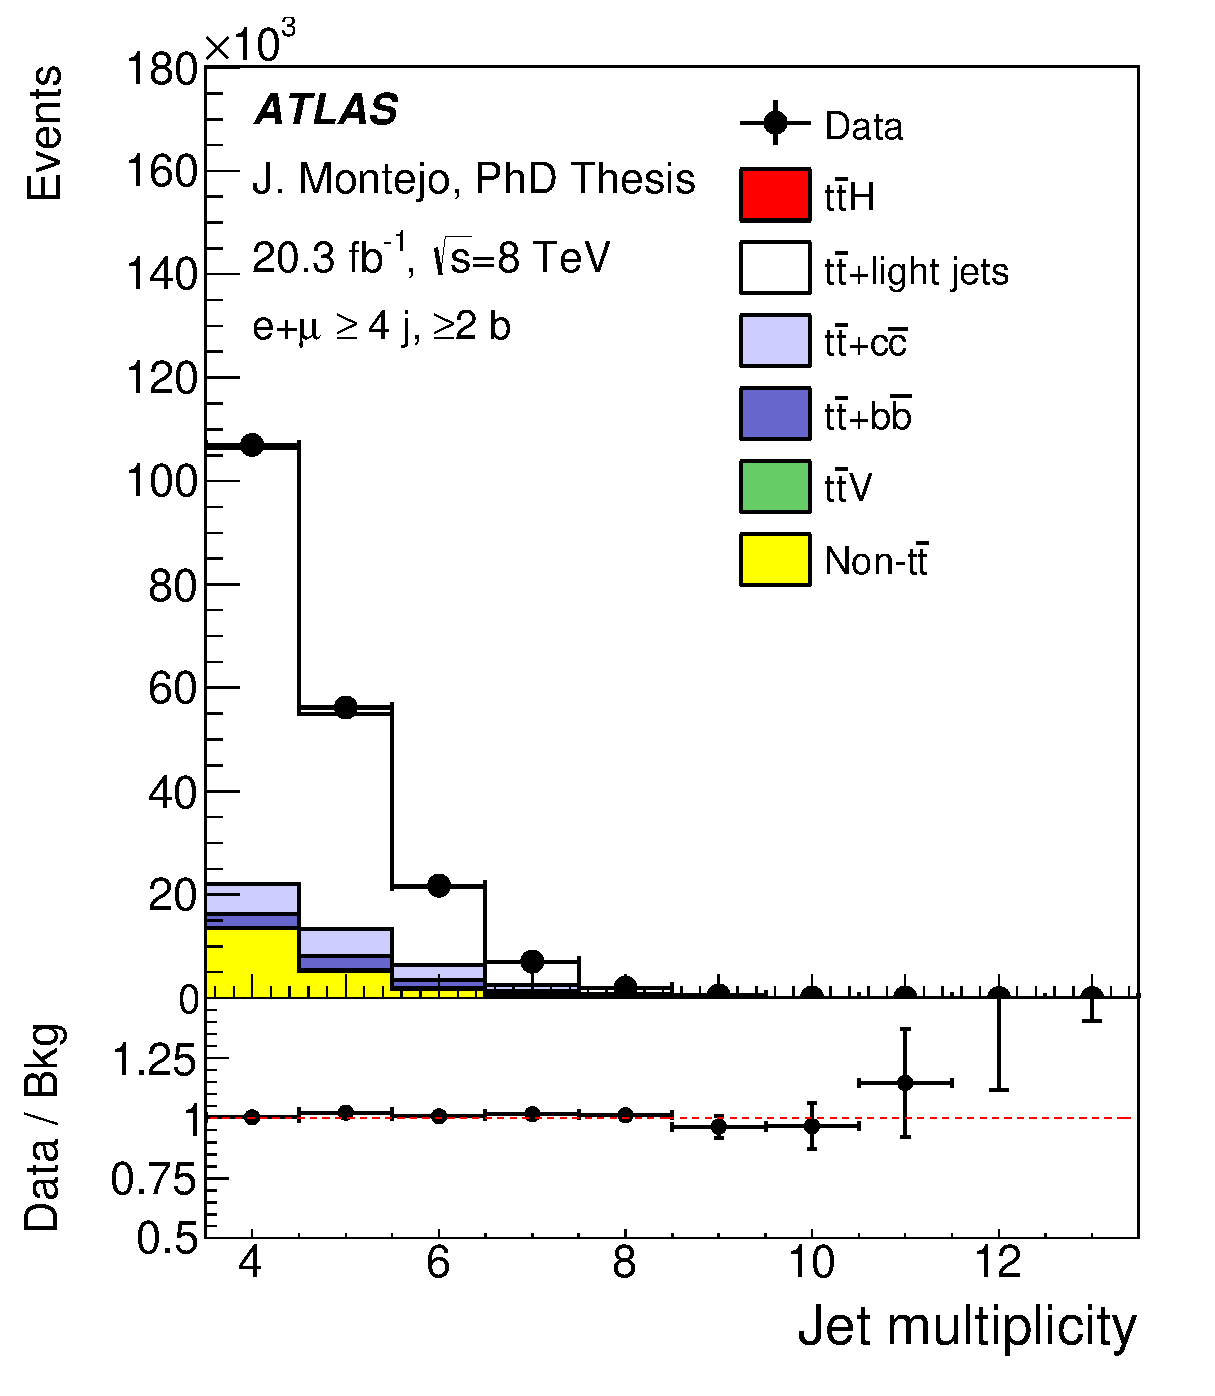
\includegraphics[width=\textwidth]{Modeling/Figures/plots_4j2b/jet_n_ELEMUON_4jetin2btagin_NOMINAL.eps}
  \caption{} \end{subfigure}
  \begin{subfigure}{0.32\textwidth}
  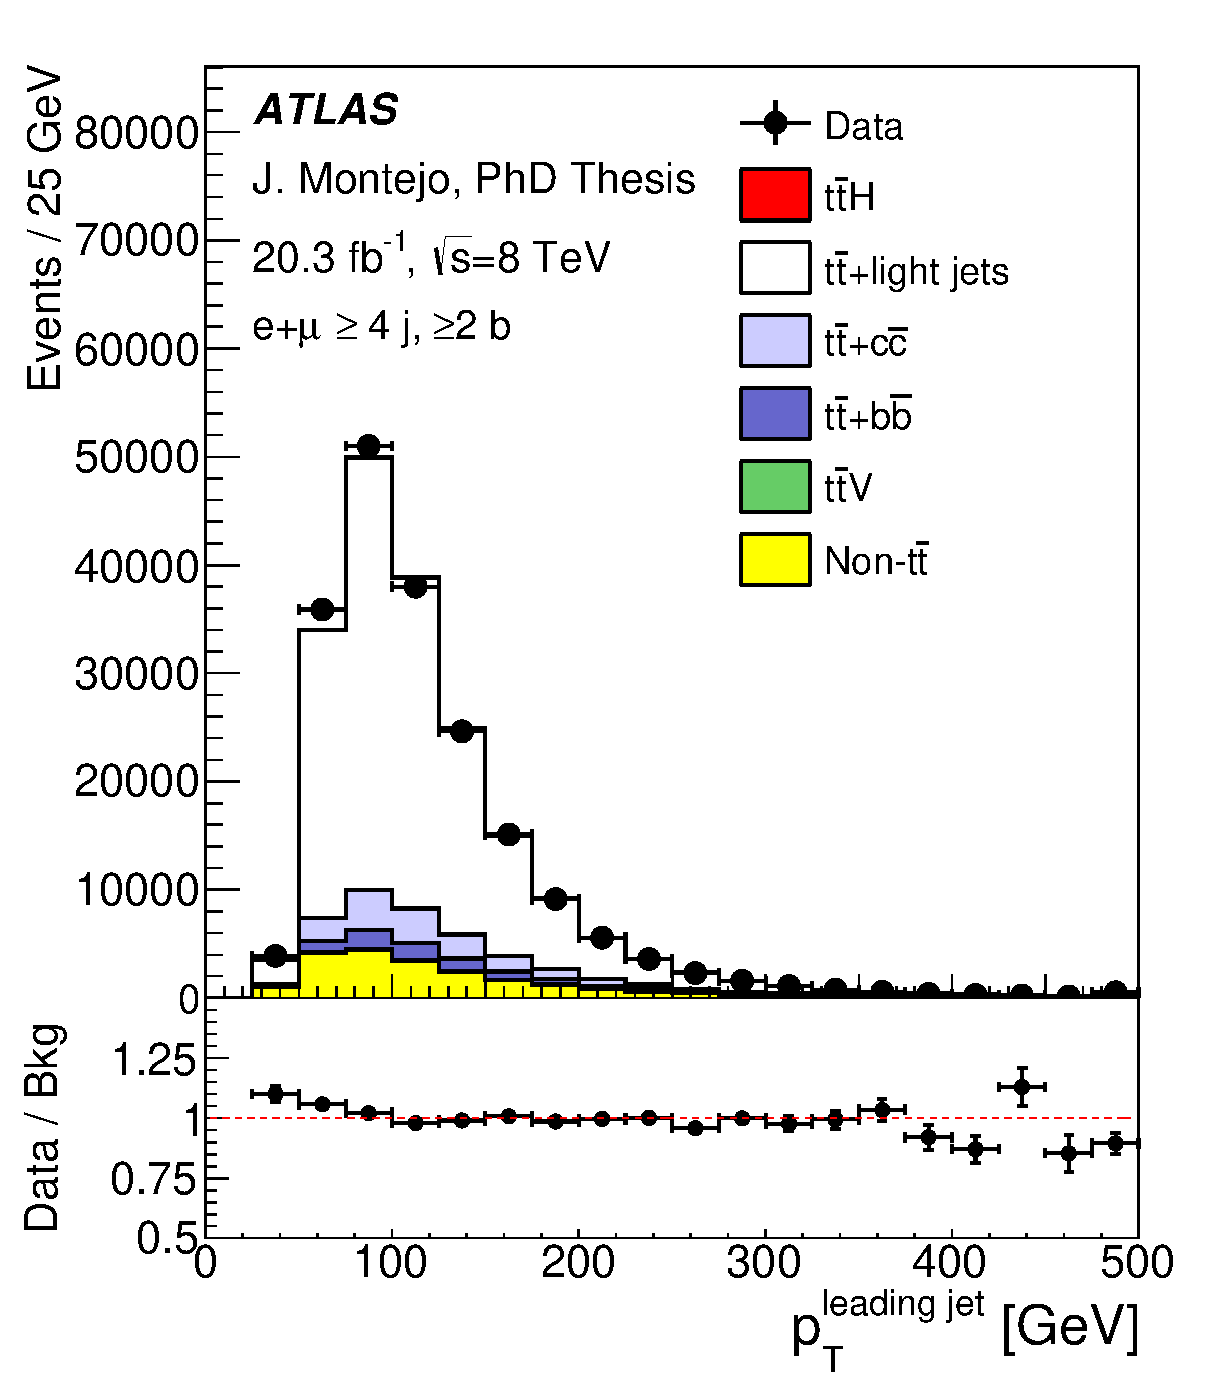
\includegraphics[width=\textwidth]{Modeling/Figures/plots_4j2b/jet1_pt_ELEMUON_4jetin2btagin_NOMINAL.eps}
  \caption{} \end{subfigure}
  \\
  \begin{subfigure}{0.32\textwidth}
  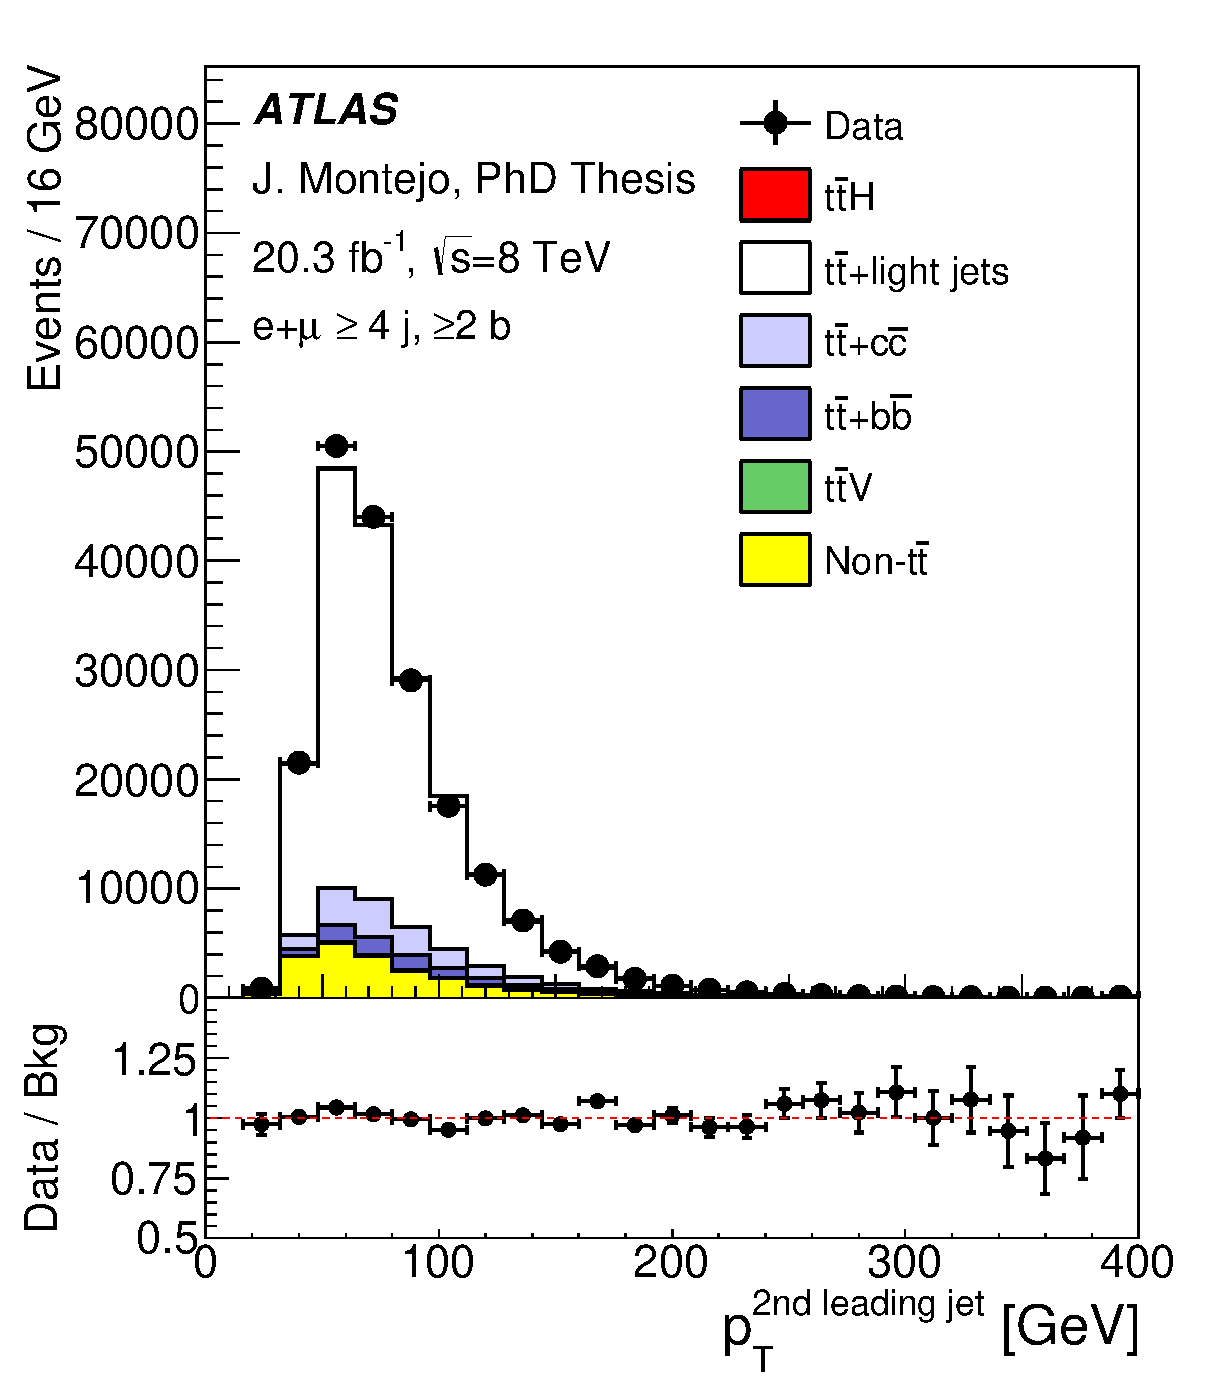
\includegraphics[width=\textwidth]{Modeling/Figures/plots_4j2b/jet2_pt_ELEMUON_4jetin2btagin_NOMINAL.eps}
  \caption{} \end{subfigure}
  \begin{subfigure}{0.32\textwidth}
  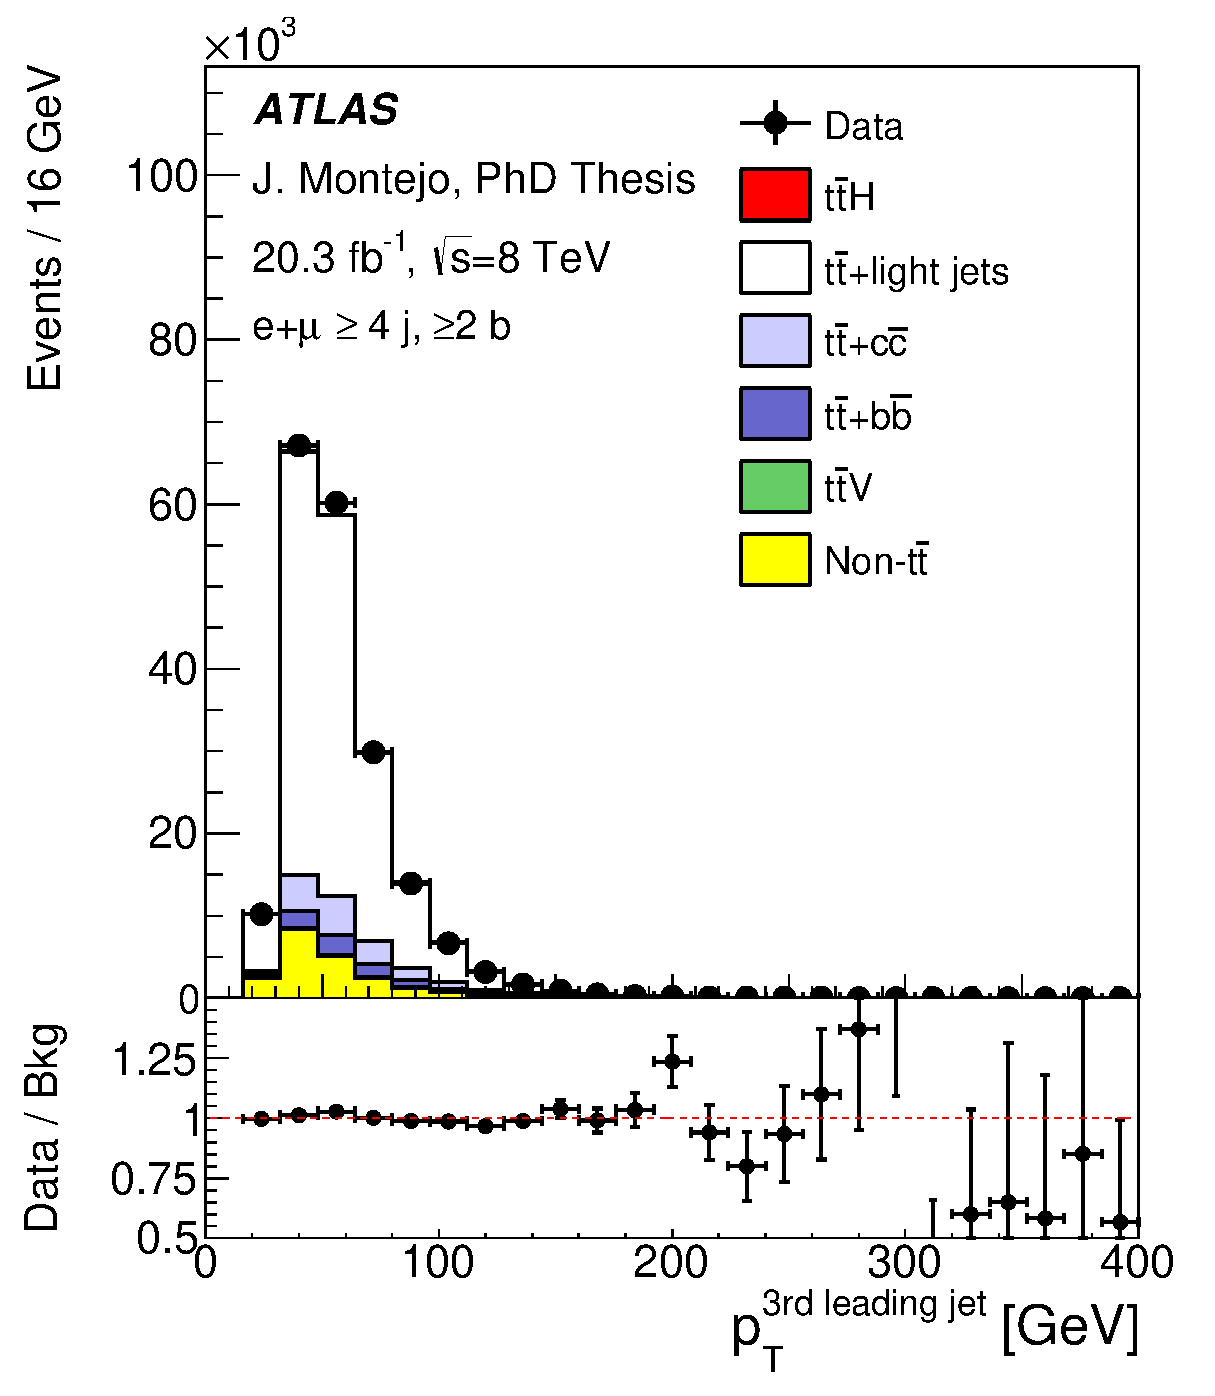
\includegraphics[width=\textwidth]{Modeling/Figures/plots_4j2b/jet3_pt_ELEMUON_4jetin2btagin_NOMINAL.eps}
  \caption{} \end{subfigure}
  \begin{subfigure}{0.32\textwidth}
  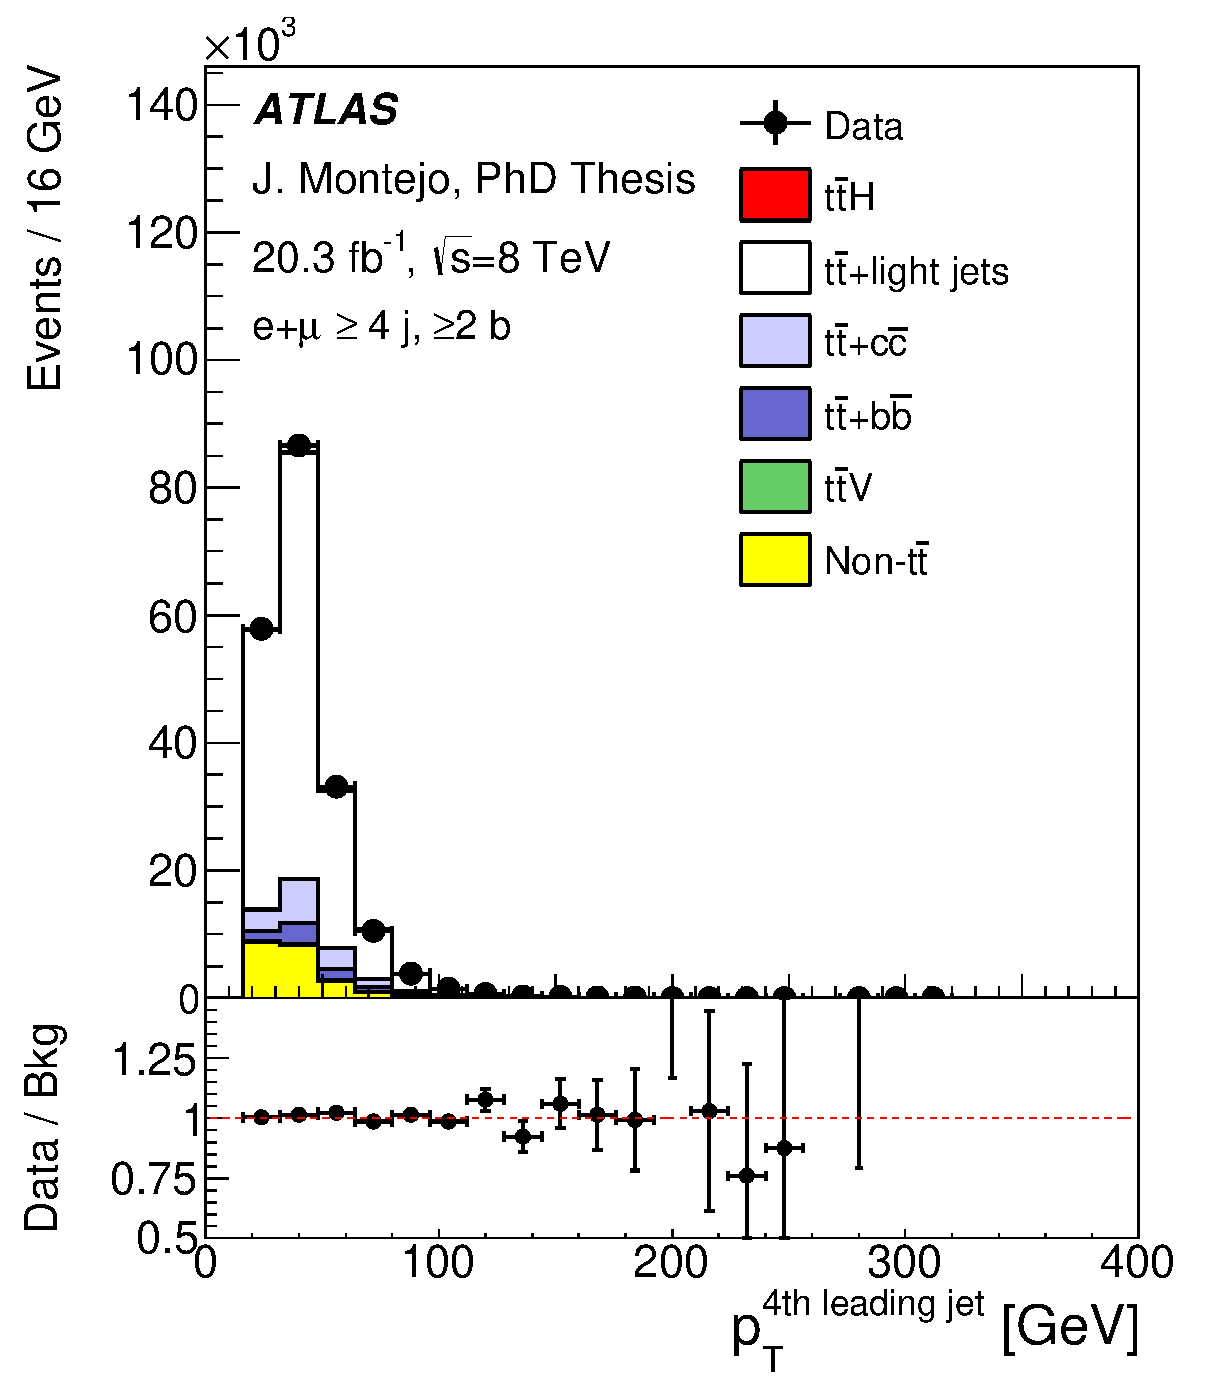
\includegraphics[width=\textwidth]{Modeling/Figures/plots_4j2b/jet4_pt_ELEMUON_4jetin2btagin_NOMINAL.eps}
  \caption{} \end{subfigure}
  \\
  \begin{subfigure}{0.32\textwidth}
  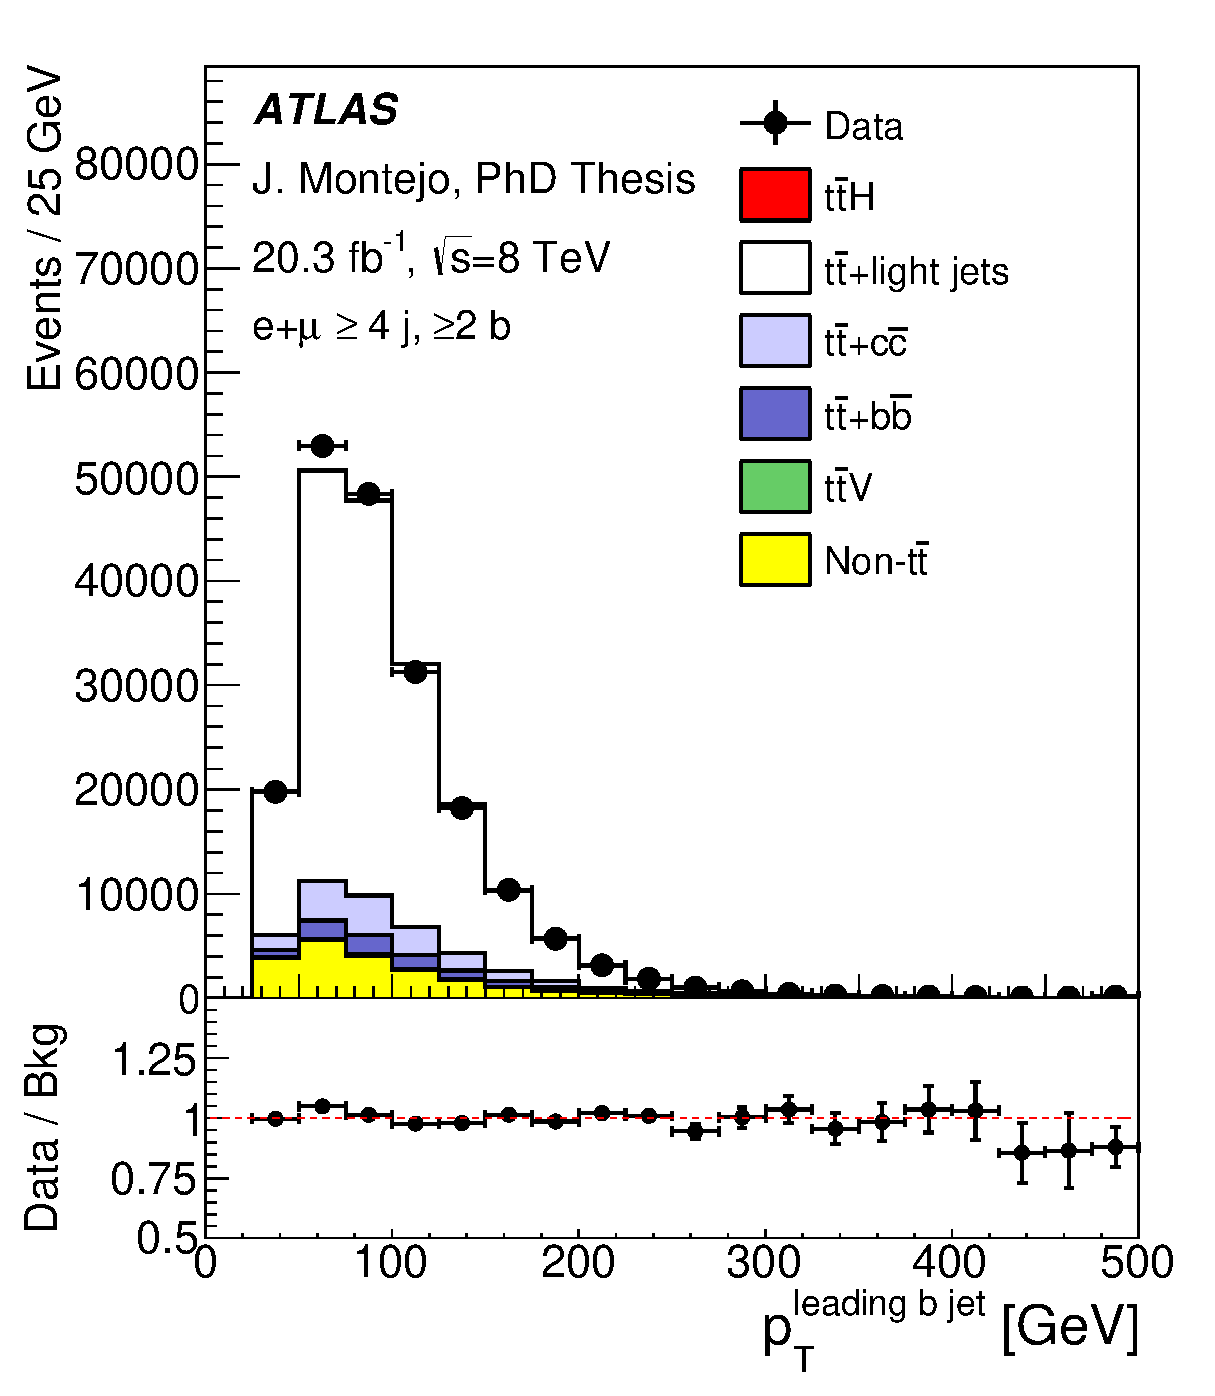
\includegraphics[width=\textwidth]{Modeling/Figures/plots_4j2b/bjet1_pt_ELEMUON_4jetin2btagin_NOMINAL.eps}             
  \caption{} \end{subfigure}
  \begin{subfigure}{0.32\textwidth}
  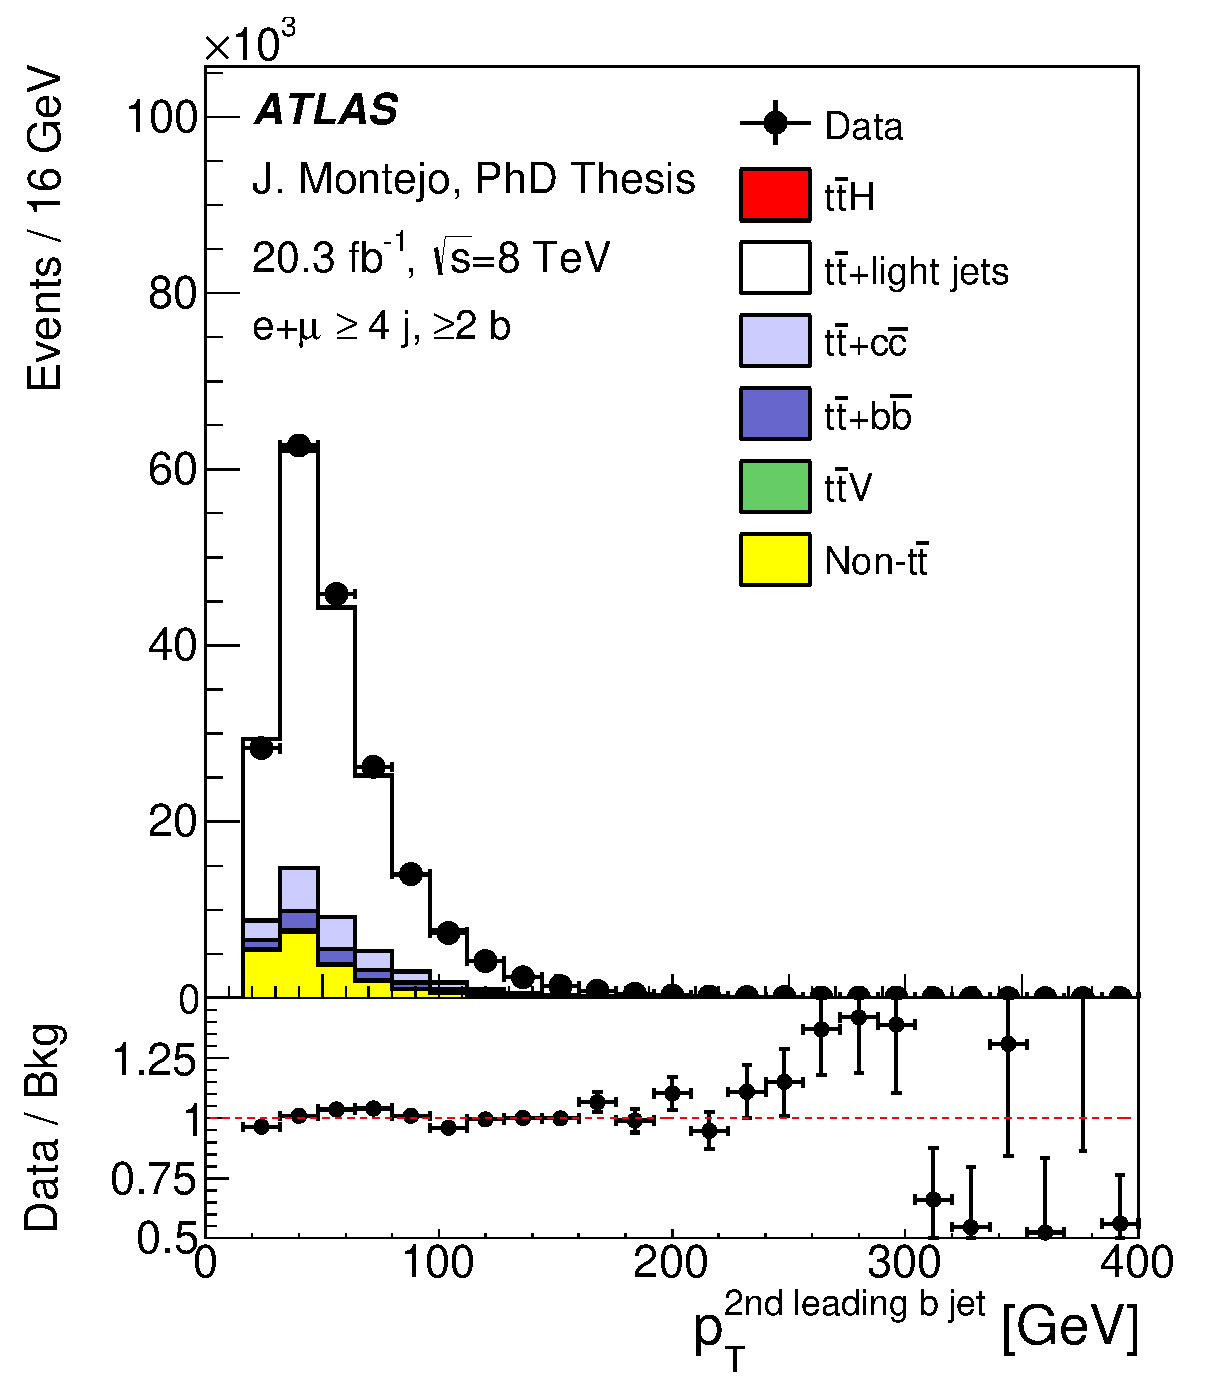
\includegraphics[width=\textwidth]{Modeling/Figures/plots_4j2b/bjet2_pt_ELEMUON_4jetin2btagin_NOMINAL.eps}             
  \caption{} \end{subfigure}
  \begin{subfigure}{0.32\textwidth}
  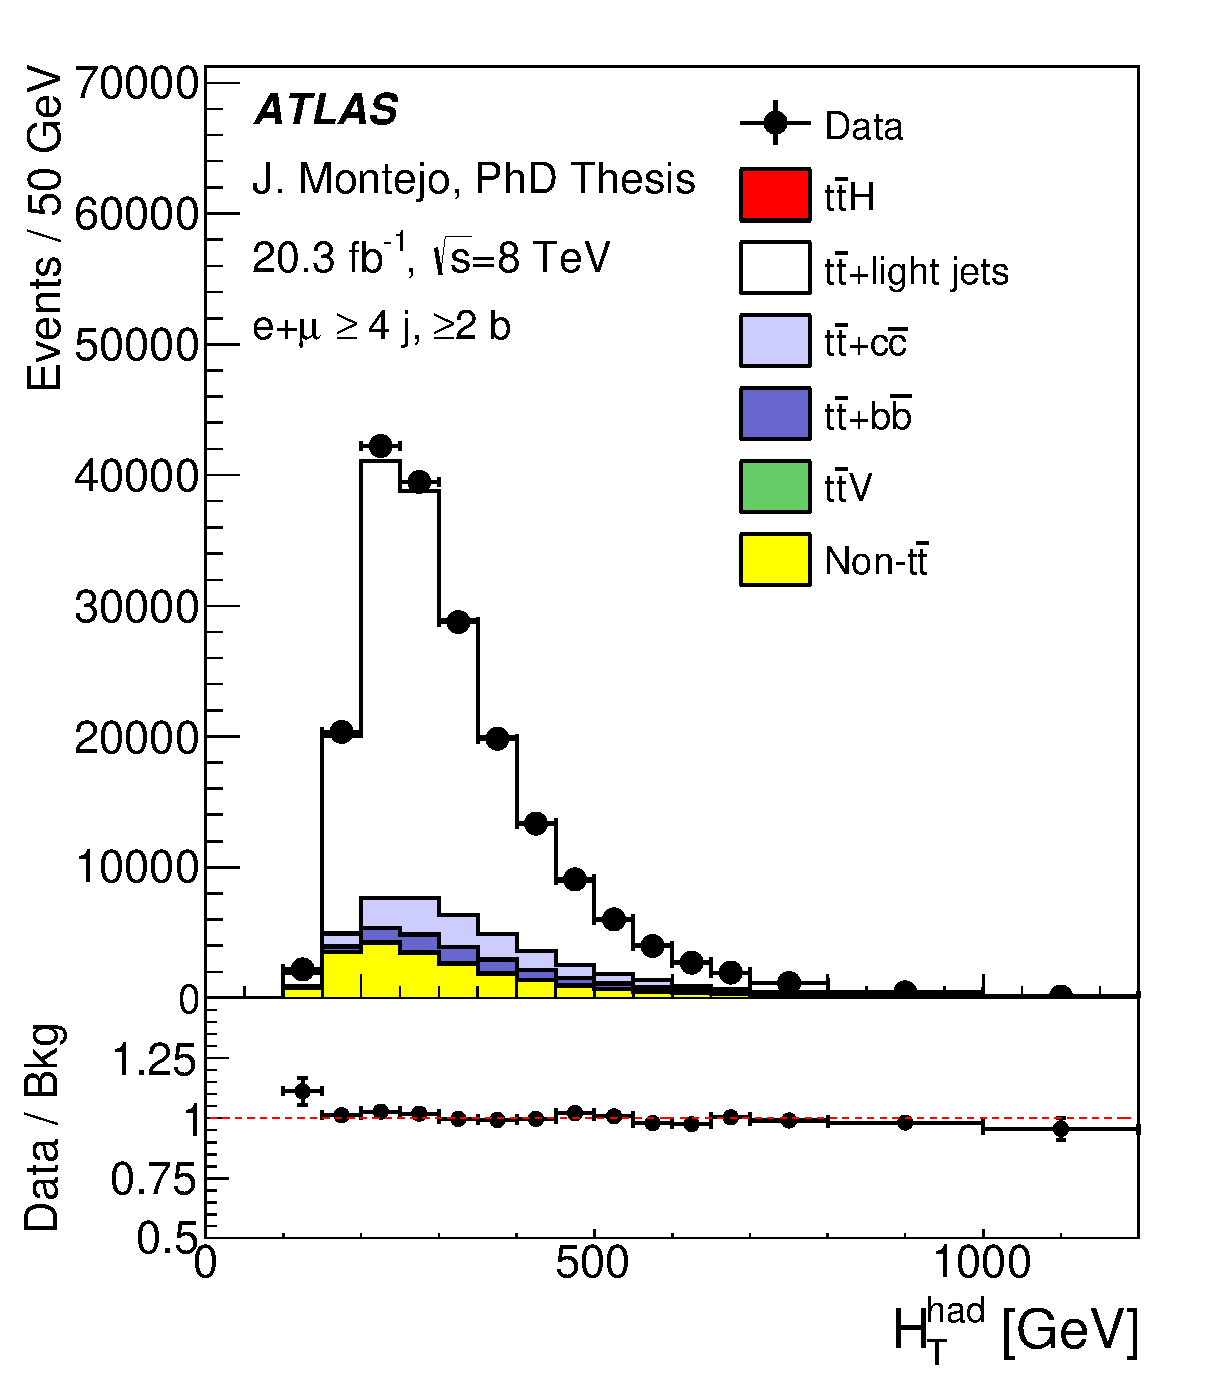
\includegraphics[width=\textwidth]{Modeling/Figures/plots_4j2b/HTj_ELEMUON_4jetin2btagin_NOMINAL.eps}                  
  \caption{} \end{subfigure}
  \caption{Comparison between data and prediction plots for (a) $b$-tag multiplicity, (b) jet multiplicity, (c) leading jet \pt, (d) second leading jet \pt, (e) third leading jet \pt, (f) fourth leading jet \pt, (g) leading $b$-tagged jet \pt, (h) second leading $b$-tagged jet \pt\ and (i) scalar sum of jet \pt: $\hthad$. }
  \label{fig:plots_1}
\end{figure}

\begin{figure}[tp!]
  \centering
  \begin{subfigure}{0.32\textwidth}
  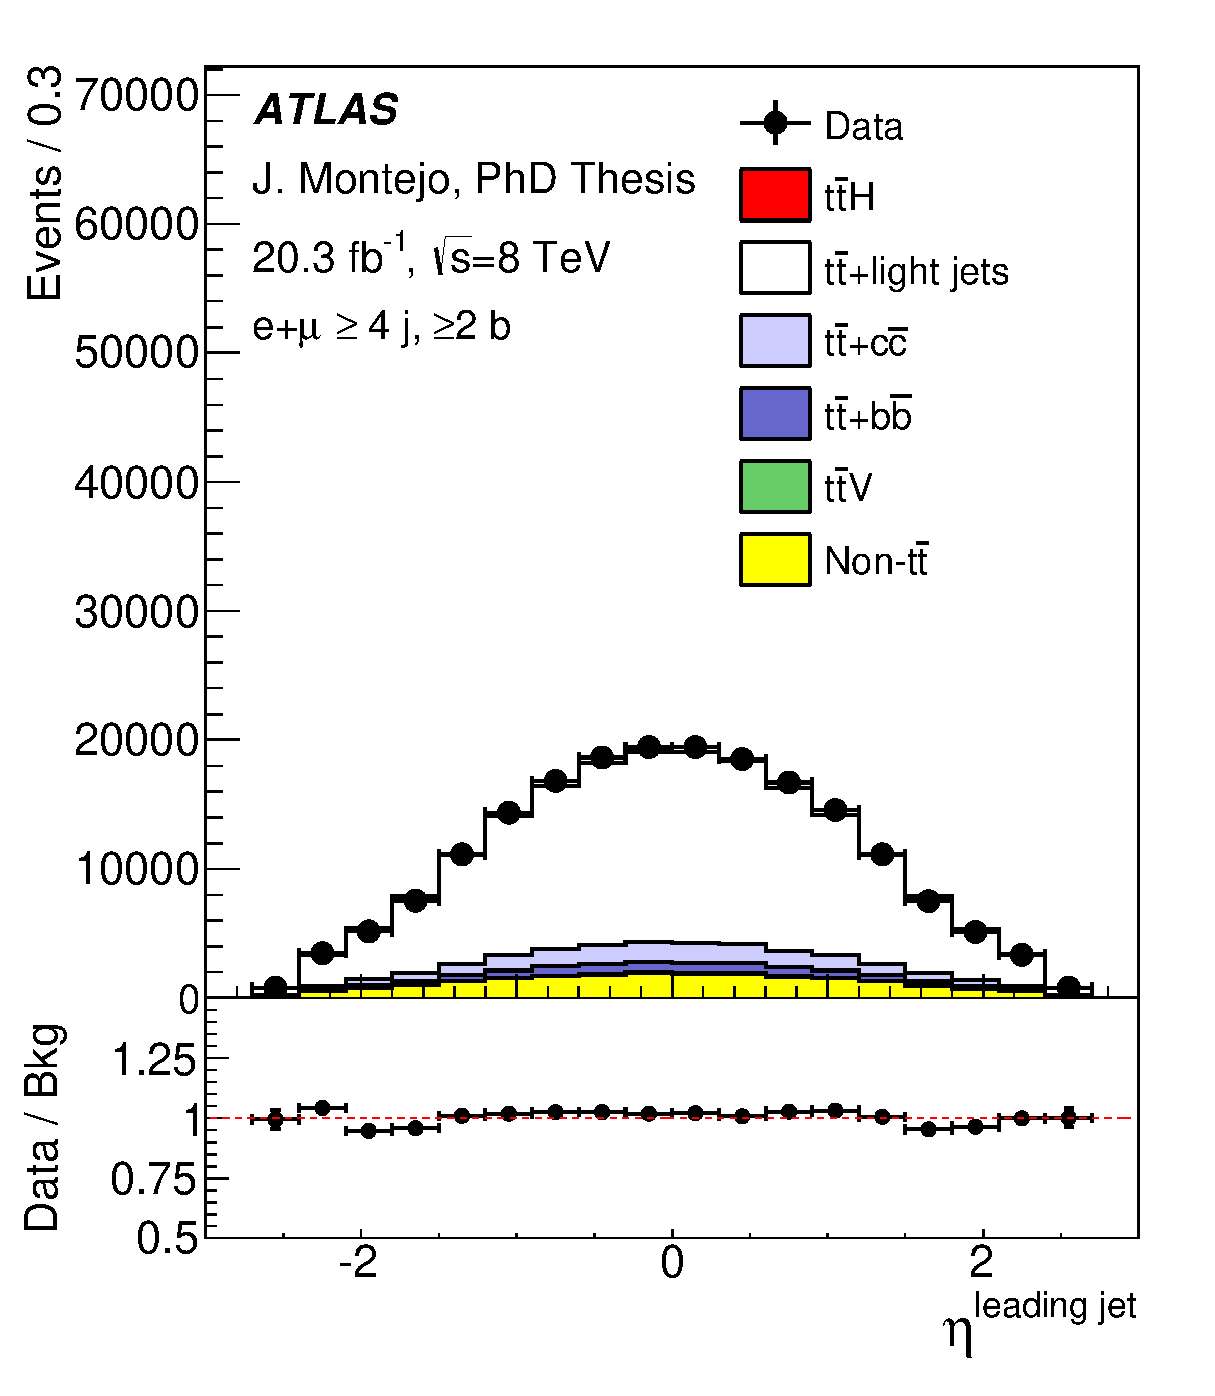
\includegraphics[width=\textwidth]{Modeling/Figures/plots_4j2b/jet1_eta_ELEMUON_4jetin2btagin_NOMINAL.eps}             
  \caption{} \end{subfigure}
  \begin{subfigure}{0.32\textwidth}
  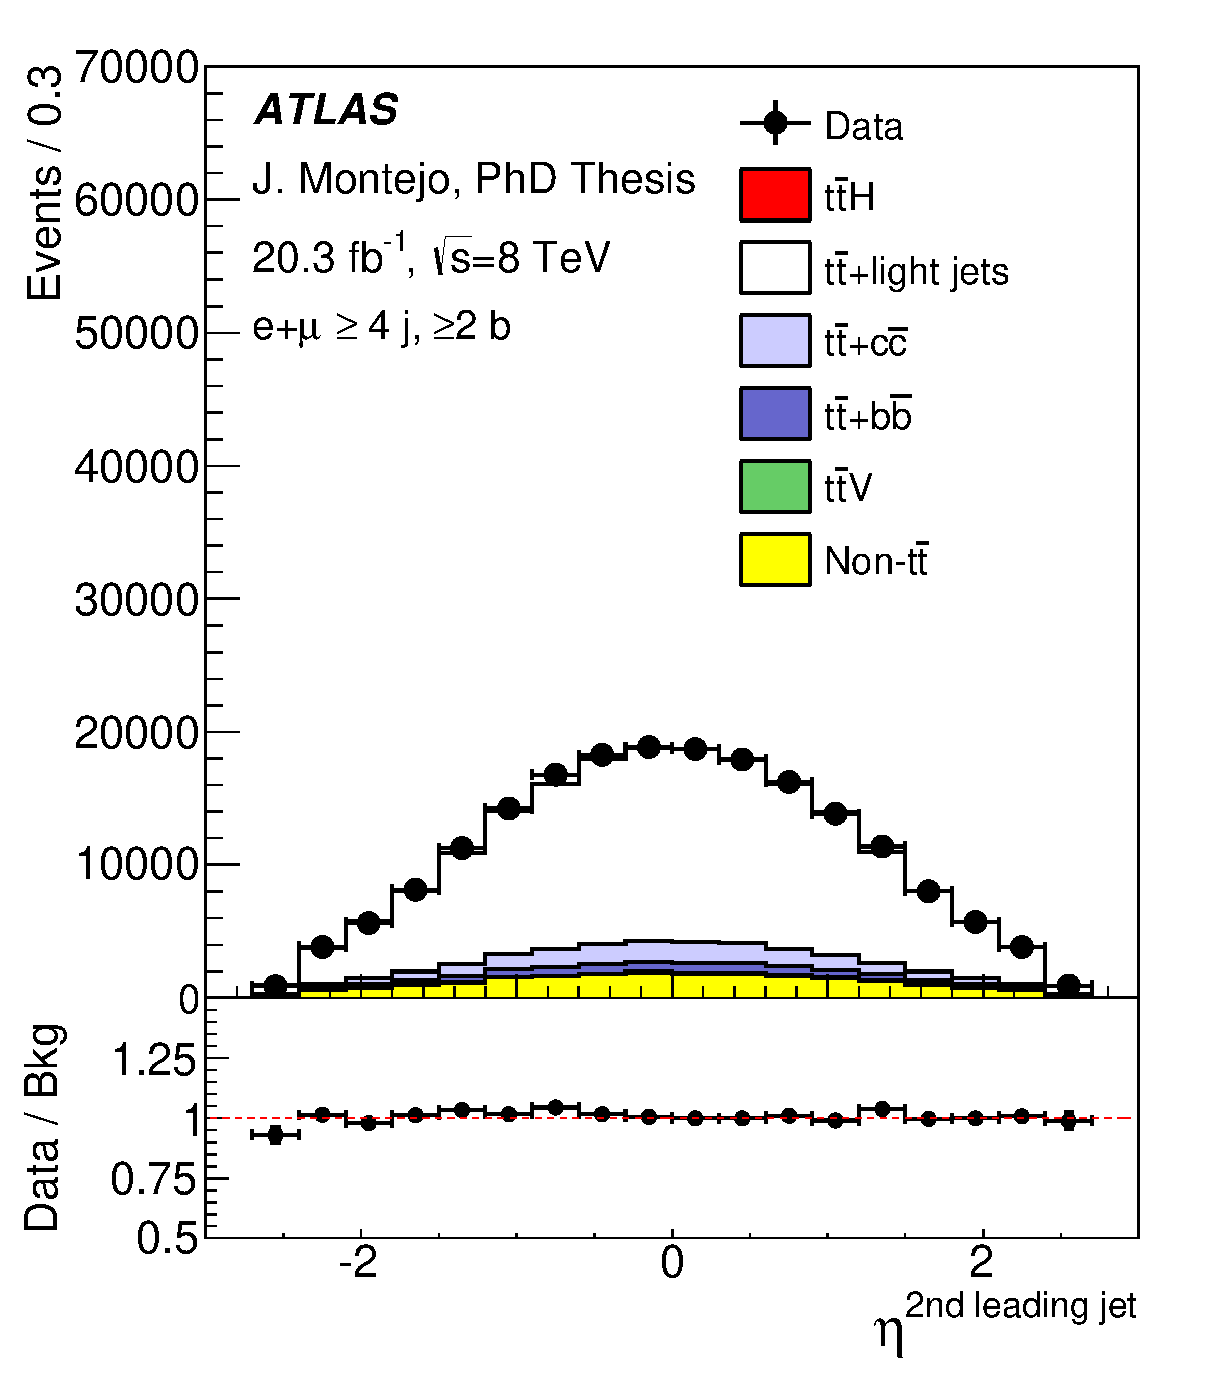
\includegraphics[width=\textwidth]{Modeling/Figures/plots_4j2b/jet2_eta_ELEMUON_4jetin2btagin_NOMINAL.eps}
  \caption{} \end{subfigure}
  \begin{subfigure}{0.32\textwidth}
  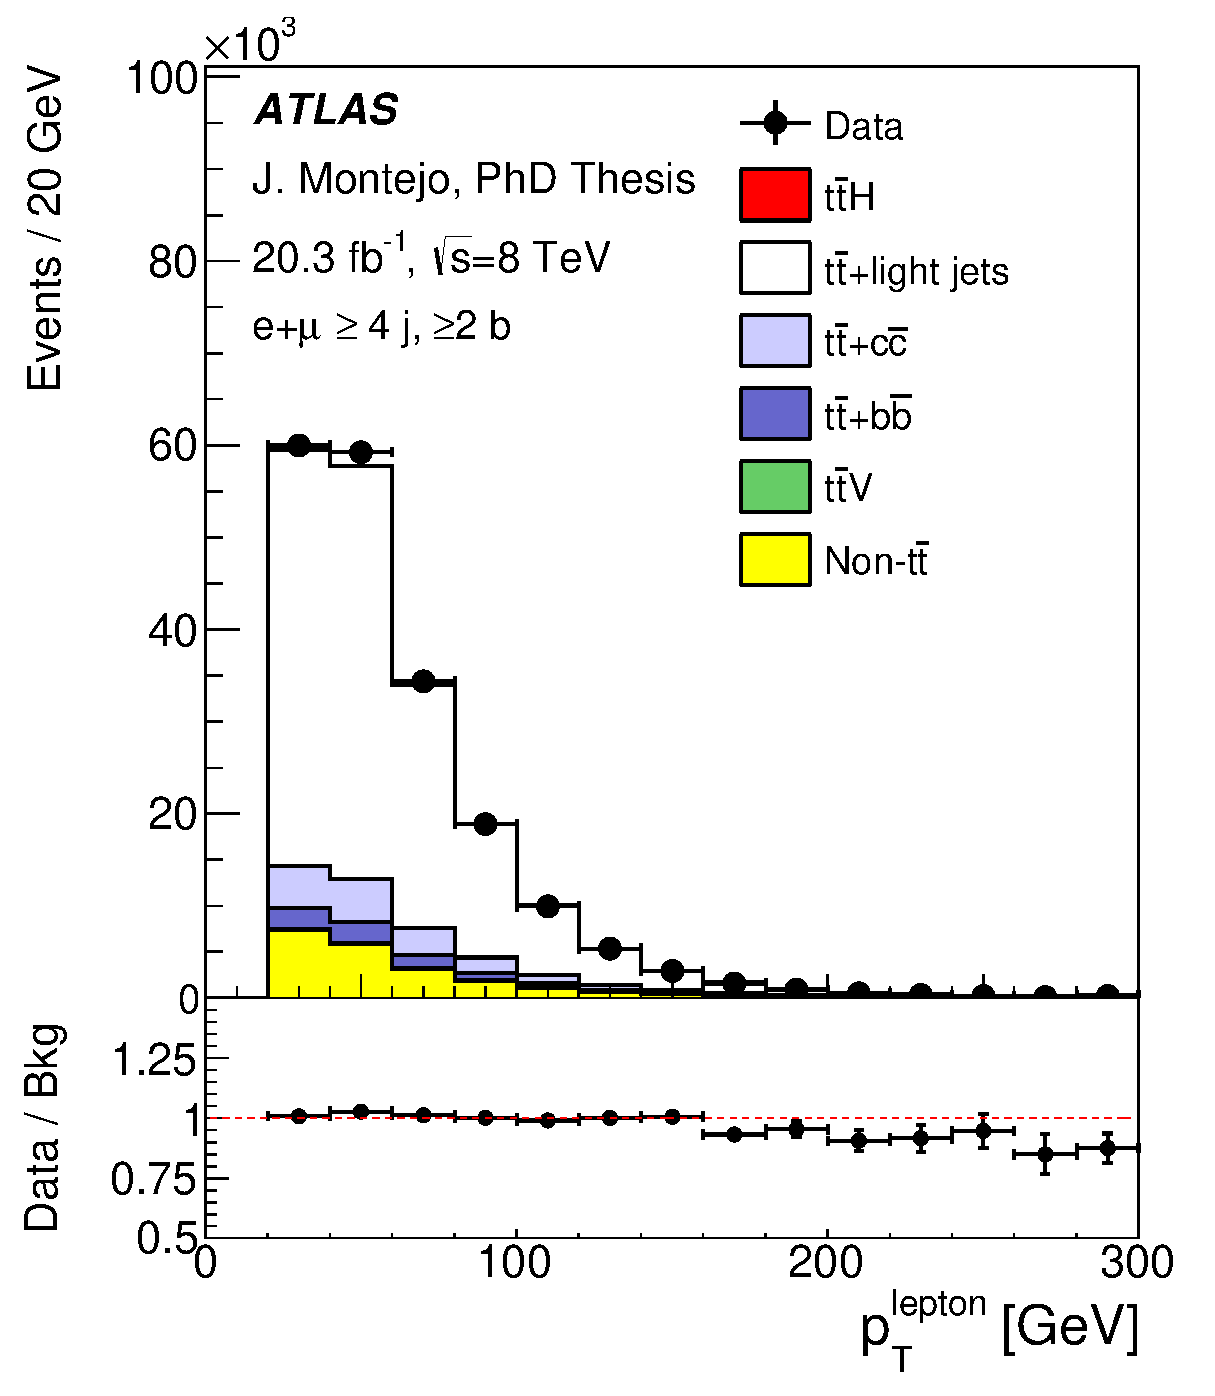
\includegraphics[width=\textwidth]{Modeling/Figures/plots_4j2b/lep_pt_ELEMUON_4jetin2btagin_NOMINAL.eps}
  \caption{} \end{subfigure}
  \\
  \begin{subfigure}{0.32\textwidth}
  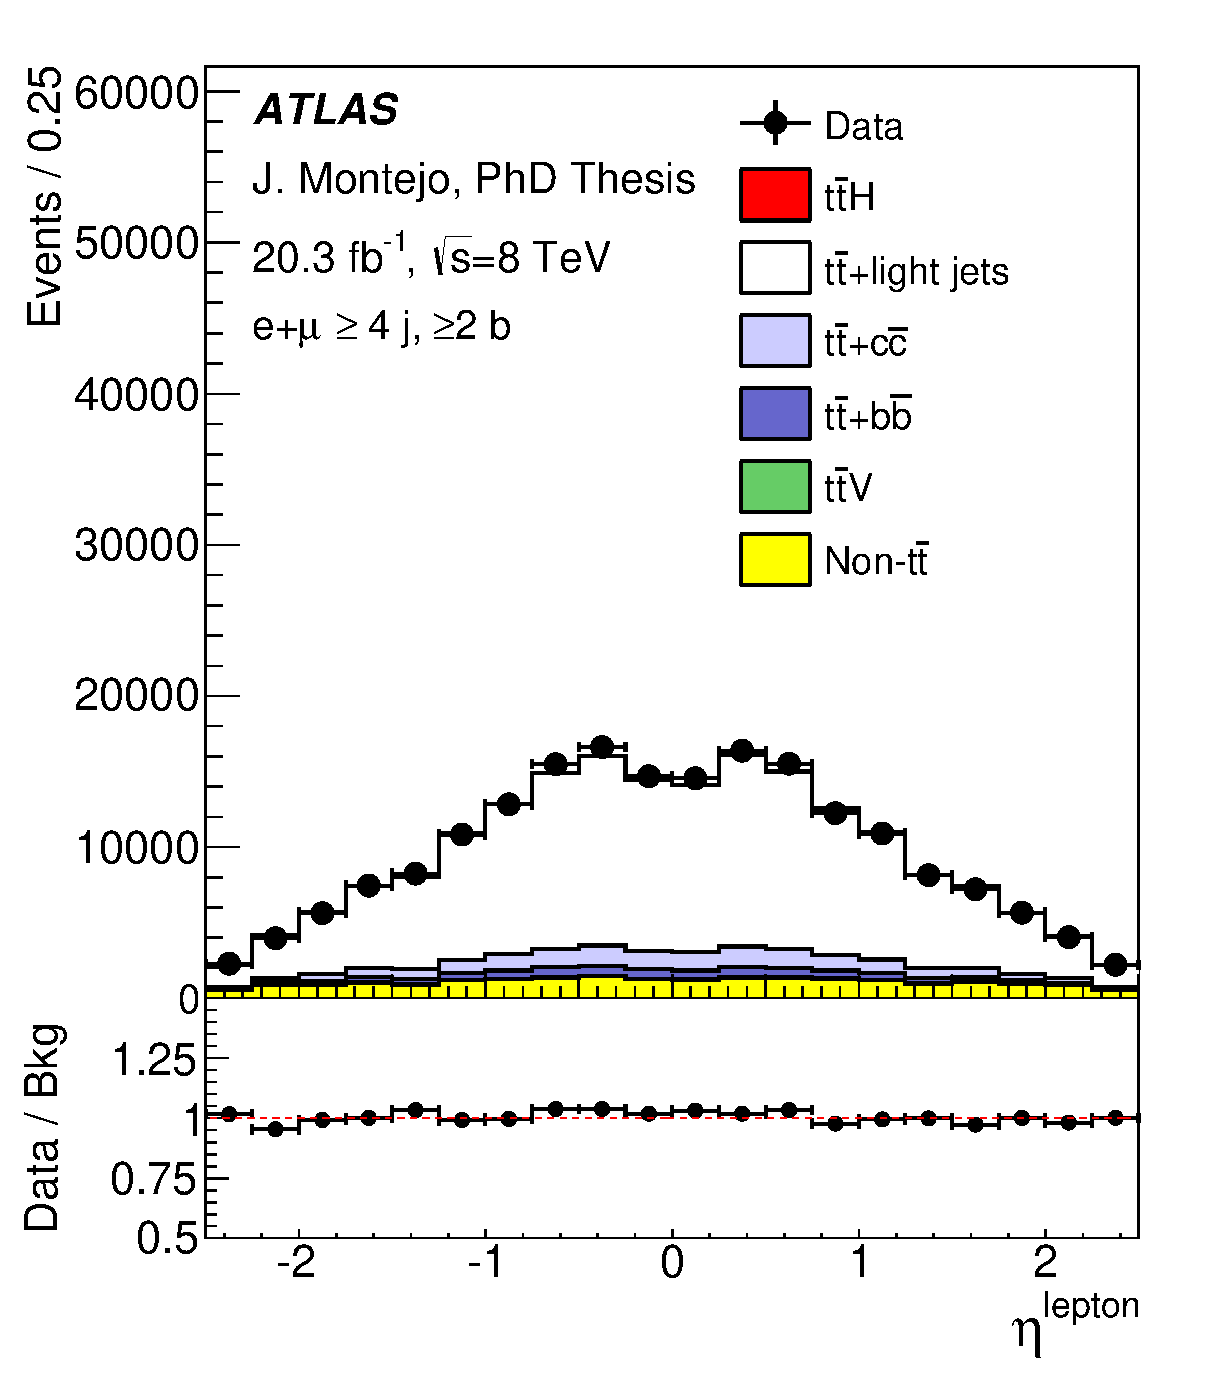
\includegraphics[width=\textwidth]{Modeling/Figures/plots_4j2b/lep_eta_ELEMUON_4jetin2btagin_NOMINAL.eps}
  \caption{} \end{subfigure}
  \begin{subfigure}{0.32\textwidth}
  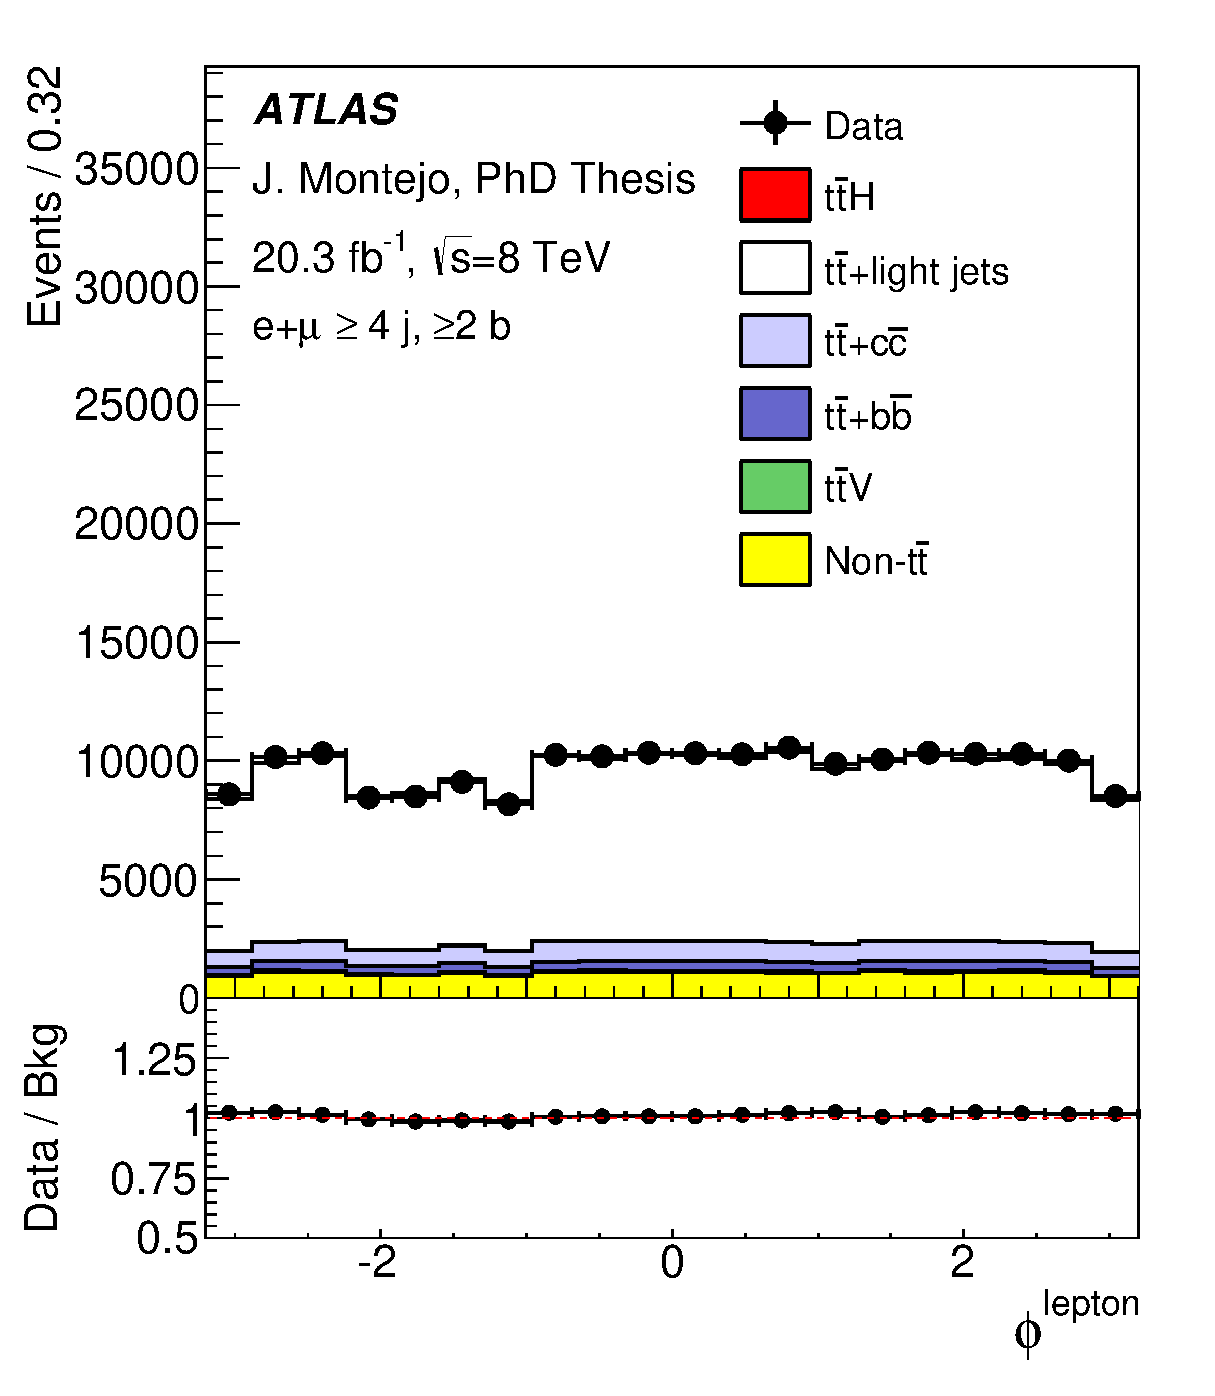
\includegraphics[width=\textwidth]{Modeling/Figures/plots_4j2b/lep_phi_ELEMUON_4jetin2btagin_NOMINAL.eps}
  \caption{} \end{subfigure}
  \begin{subfigure}{0.32\textwidth}
  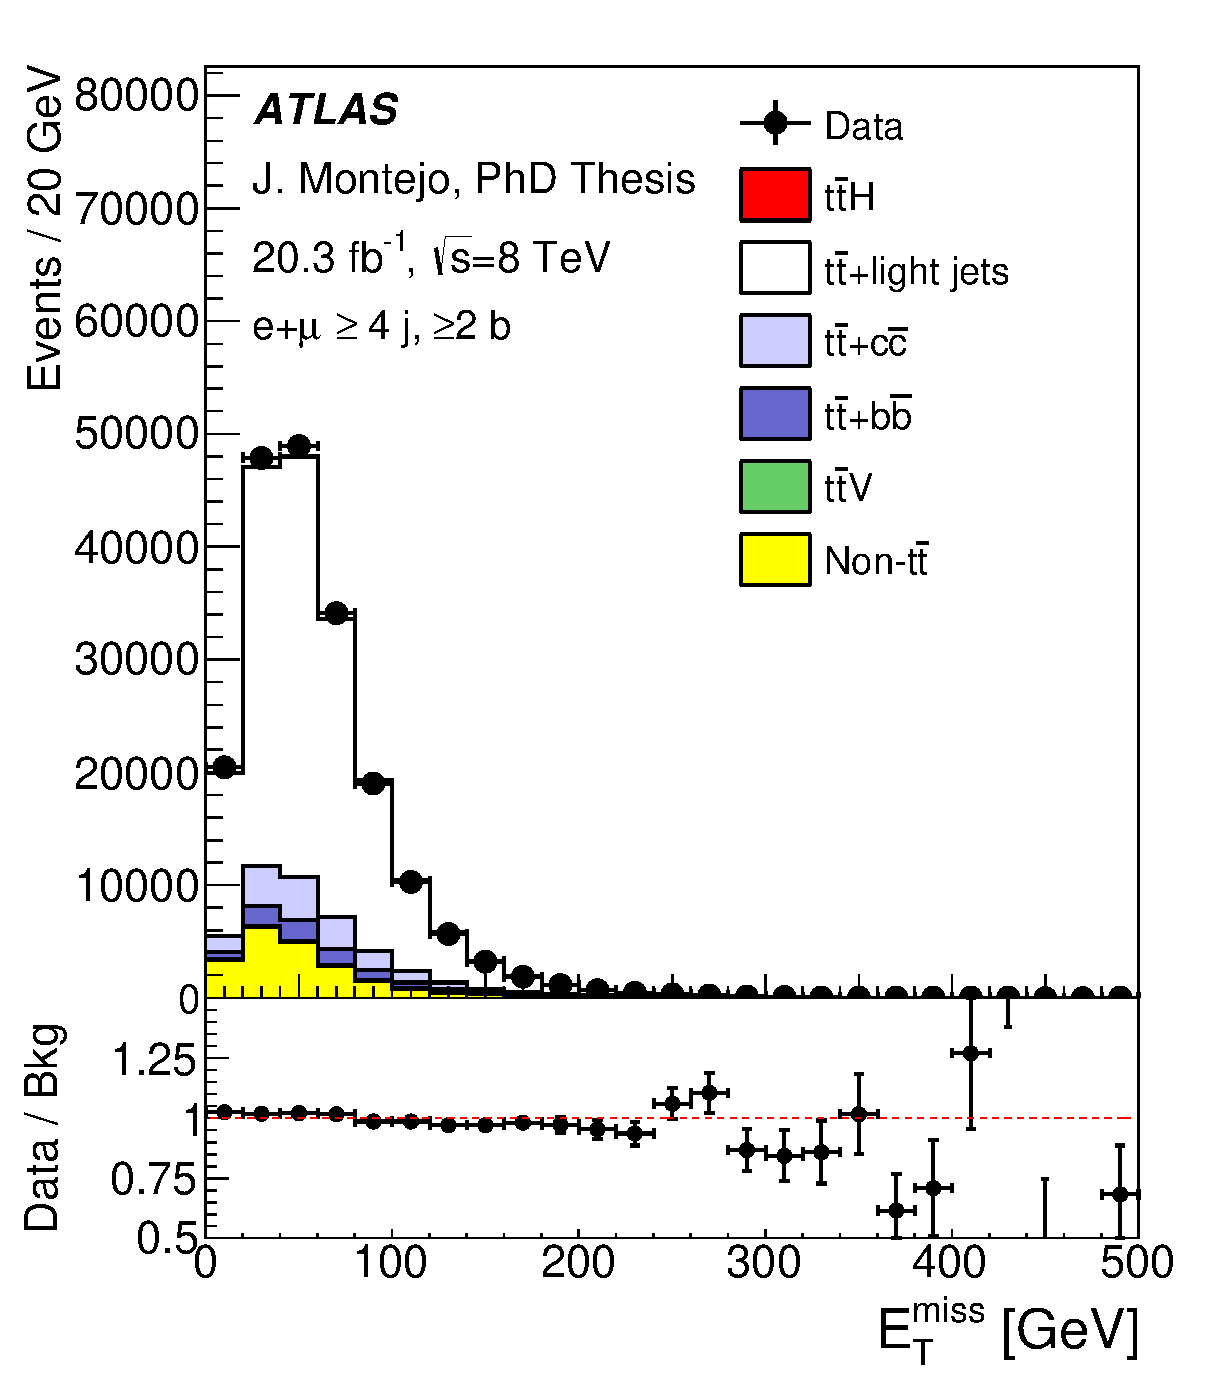
\includegraphics[width=\textwidth]{Modeling/Figures/plots_4j2b/met_ELEMUON_4jetin2btagin_NOMINAL.eps}
  \caption{} \end{subfigure}
  \\
  \begin{subfigure}{0.32\textwidth}
  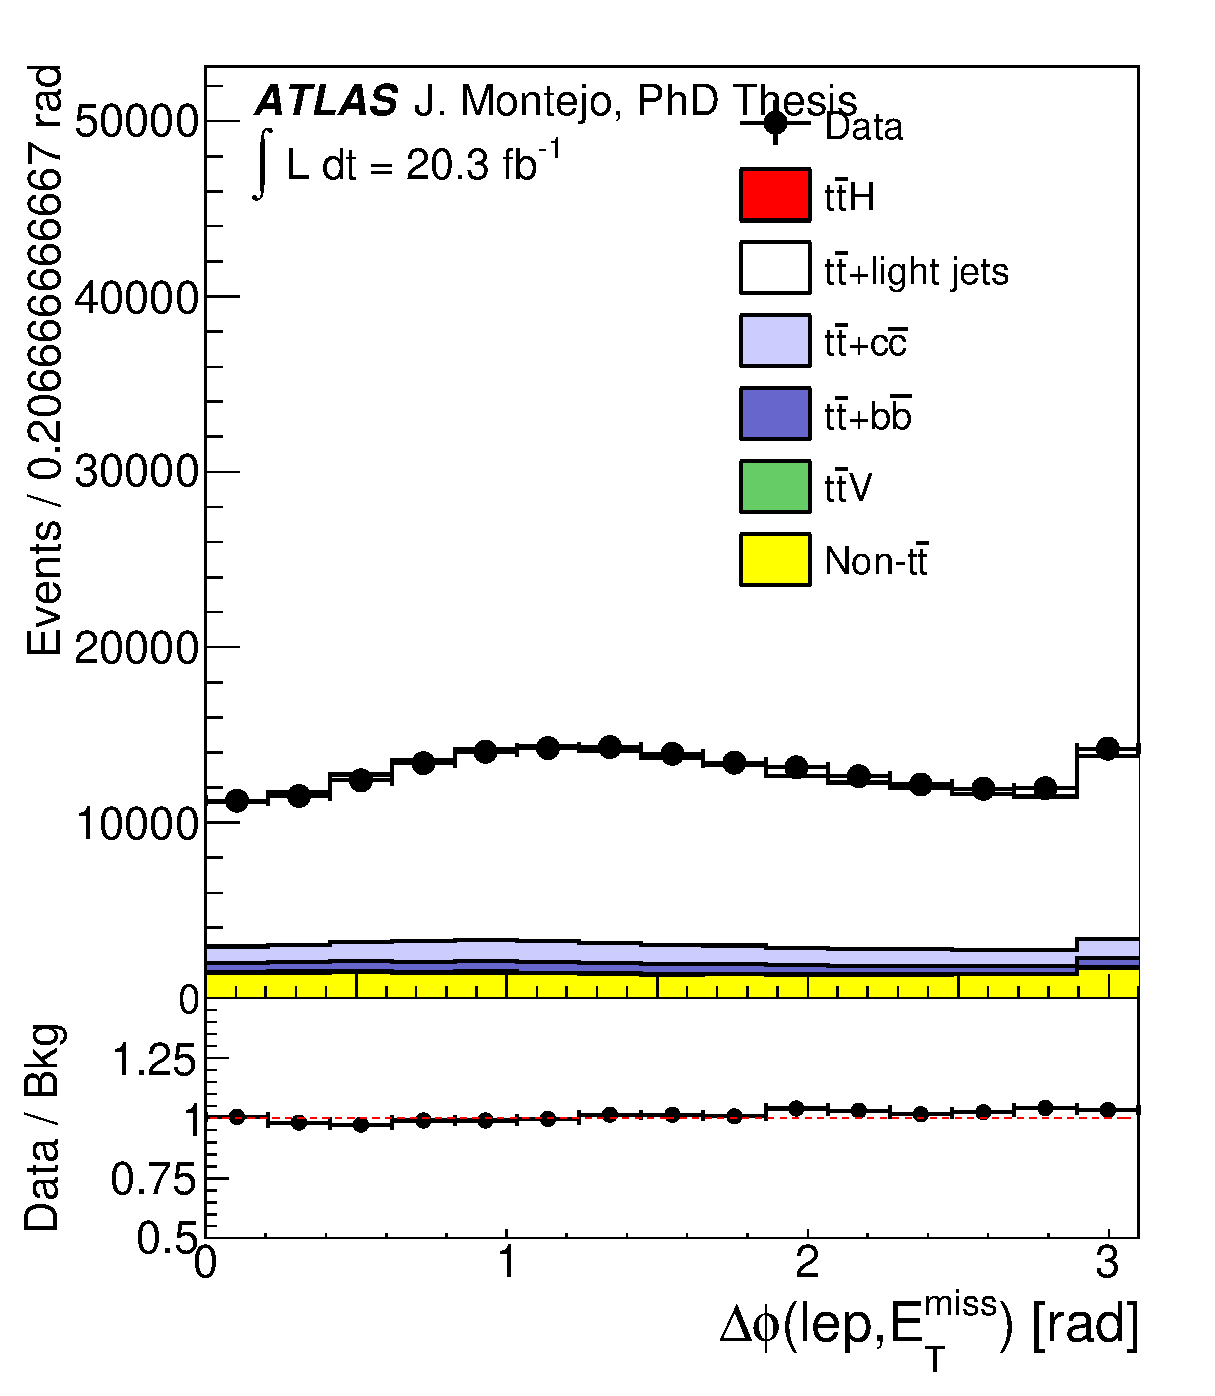
\includegraphics[width=\textwidth]{Modeling/Figures/plots_4j2b/deltaPhi_lep_MET_ELEMUON_4jetin2btagin_NOMINAL.eps}     
  \caption{} \end{subfigure}
  \begin{subfigure}{0.32\textwidth}
  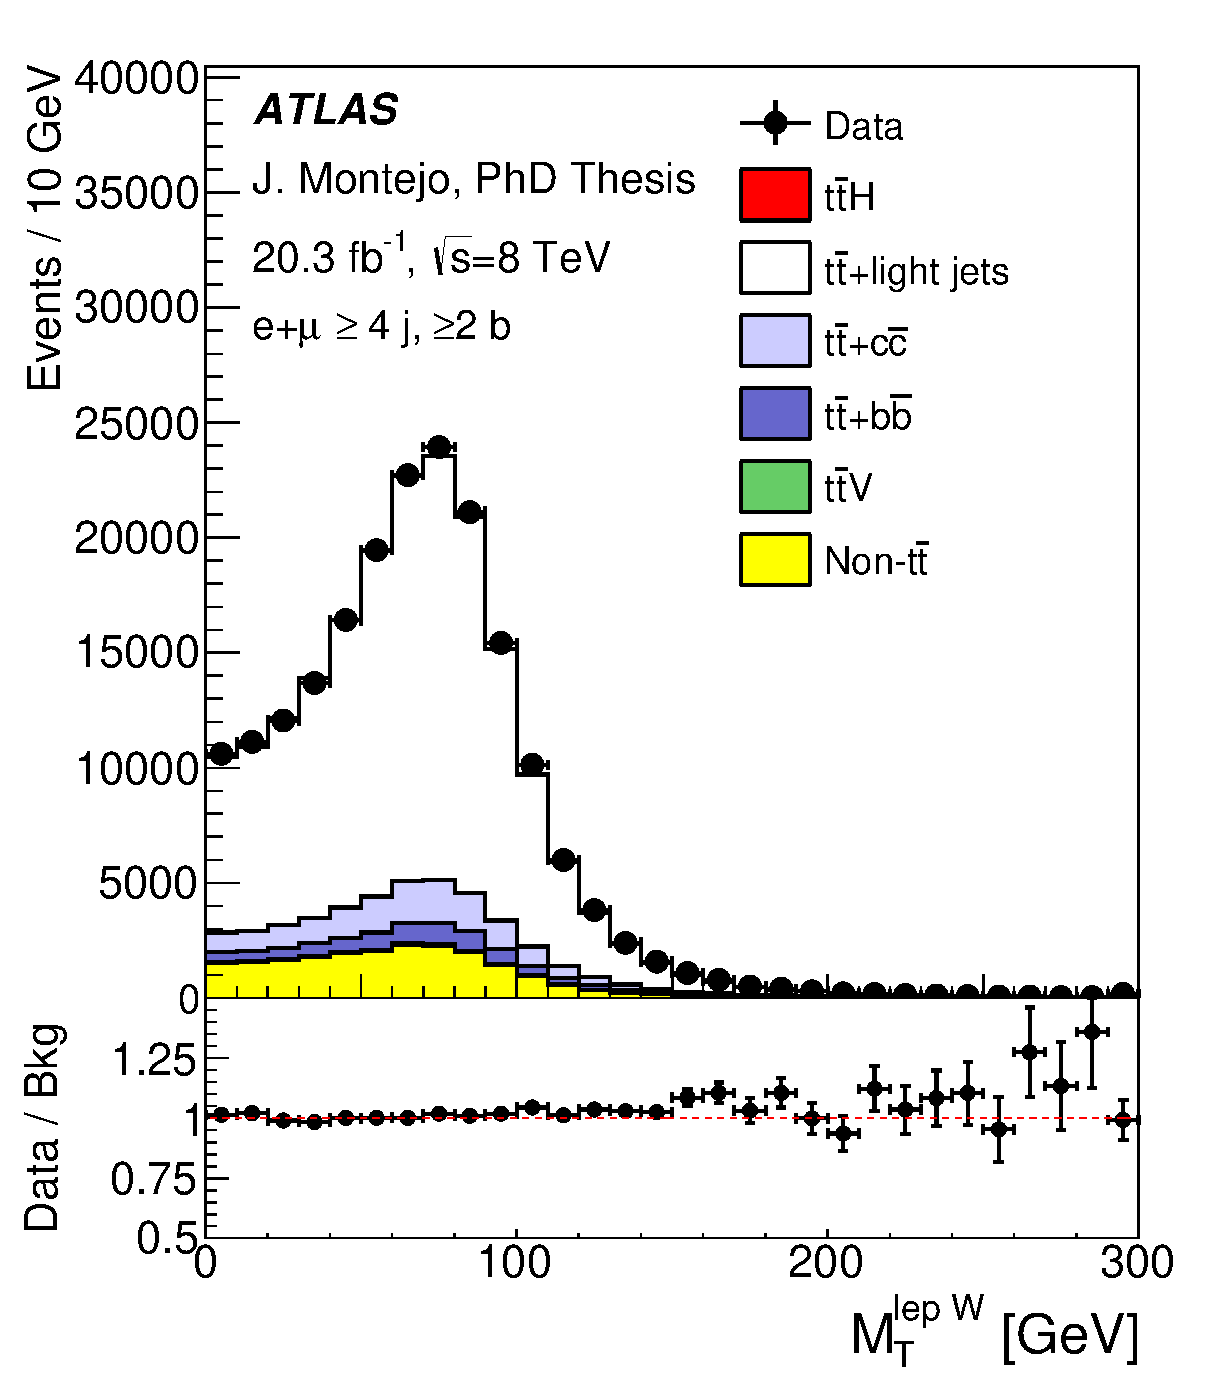
\includegraphics[width=\textwidth]{Modeling/Figures/plots_4j2b/WlepMT_ELEMUON_4jetin2btagin_NOMINAL.eps}               
  \caption{} \end{subfigure}
  \begin{subfigure}{0.32\textwidth}
  \includegraphics[width=\textwidth]{Modeling/Figures/plots_4j2b/HTAll_ELEMUON_4jetin2btagin_NOMINAL.eps}                
  \caption{} \end{subfigure}
  \caption{Comparison between data and prediction plots for (a) leading jet $\eta$, (b) second leading jet $\eta$, (c) lepton \pt, (d) lepton $\eta$, (e) lepton $\phi$, (f) missing transverse energy \met, (g) $\Delta\phi$ between the lepton and \met, (h) transverse mass of the $W$ boson \mtw\ and (i) scalar sum of jet \pt, lepton \pt\ and \met: $\HT$. }
  \label{fig:plots_2}
\end{figure}


\section{Tag rate function method}
%The chosen $b$-tagging operating point provides an average efficiency of \unit[70]{\%} tagging jets originating from $b$-quarks and a $<\unit[1]{\%}$ mistag rate. 
%The requirement of a large number of $b$-tagged jets translates into a very low acceptance, especially for backgrounds with low number of $b$-quarks, leading to a severe impact on the available MC statistics.
%The low statistic in the MC templates has a negative impact on the sensitivity of the analysis
%and leads to unreliable estimates of the effect of systematic uncertainties.

When requiring a high number of $b$-tags in the analysis, the number of available MC events is significantly reduced, leading to large fluctuations in the resulting distributions. This can negatively affect the sensitivity of the analysis through the large statistical uncertainties on the templates and unreliable systematic uncertainties due to shape fluctuations. The loss in statistics is especially severe in the backgrounds that reach the high $b$-tag multiplicities via mistags, since the mistag rate is $<\unit[1]{\%}$.

In order to mitigate this problem, the \textit{tag rate function} (TRF) method is introduced. 
Instead of tagging the MC jets with the output of the $b$-tagging algorithm, their probabilities of being $b$-tagged are computed based on parameterized efficiencies. Events are weighted according to their probability of containing the required number of $b$-tags.
The $b$-tagging efficiencies are extracted from \ttbar\ events as a function of the jet \pT, \abseta\ and flavor of the jet, $\varepsilon (\pt,\abseta,f)$.\footnote{
The MC jet flavor is defined by looking at partons with $\pT>\unit[5]{\gev}$ within a $\DR<0.3$ cone around the jet direction.
If a $b$-quark is found, the jet is labeled with $b$ origin. If no $b$-quarks are found, $c$-quarks are considered. If no $c$-quarks are found either, a jet is labeled as a light jet.}
An additional tagging dependency is introduced in \ttbar\ events in order to consider the production mechanism of the jet. This refinement takes into account the difference in $b$-tagging efficiency for jets originating from top decay products, additional heavy-flavor jets and MPI jets. The $b$-tagging efficiency, averaged over \pT\ and \abseta, for the different types of jets is summarized in table~\ref{tab:btag_eff}.

\begin{table}[!t]
\centering
\begin{tabular}{ c c c }
\toprule
\toprule
%\multicolumn{3}{c}{\ttbarpt}  \\
Jet flavor & Origin & Efficiency [\%]  \\
\midrule
\multirow{3}{*}{$b$-jet} & top decay       & 72 \\
                         & additional jets & 66 \\
                         & MPI             & 49 \\
\midrule
\multirow{2}{*}{$c$-jet} & $W$ decay         & 22 \\
                         & additional jets & 18 \\
\midrule
\multirow{2}{*}{light-jet} & $W$ decay or    & \multirow{2}{*}{0.7} \\
                         & additional jets &  \\
\bottomrule
\bottomrule
\end{tabular}
\caption{
Average $b$-tagging efficiency for jets with different origins.
}
\label{tab:btag_eff}
\end{table}

For a given requirement on the number of $b$-tagged jets in the events ($n_b$), all the possible permutations of labeling $n_b$ jets as ``tagged'' are considered. 
For each permutation, a weight is applied to each jet: jets considered ``tagged'' are assigned a weight equal to the tagging probability, jets considered as ``un-tagged'' are assigned a weight equal to one minus the tagging efficiency. 
Multiplying all jet weights gives the probability for that event to contain the selected number of tags, independently of the number of jets selected by the $b$-tagging algorithm.

As an example, for a given event with $N$ jets, the probability of containing exactly one $b$-tagged jet can be computed as:
\begin{equation}
	P_{=1} = \sum\limits_{i=1}^N \left( \varepsilon_{i} \prod\limits_{i \neq j} \left( 1 - \varepsilon_{j} \right) \right)
\end{equation}
and in general the probability for inclusive $b$-tagging selections can be computed as:
\begin{equation}
  P_{\geq 1} = 1 - P_{=0}~,
\end{equation}
where $P_{=0}$ is the probability that the event contains exactly zero $b$-tags.


This allows the use of all events in the pre-$b$-tagged sample to predict the normalization and shape after any $b$-tagging selection.
The shape of the distributions built using $b$-tagged jet information is reproduced by randomly choosing one of the possible permutations based on their relative probability.

The TRF method relies on two main assumptions:
\begin{itemize}
  \item The probability of tagging a jet is independent of the rest of the jets in the event. In this way the tagging probability in an event can be factorized into the product of the probabilities of the individual jets. It should be noted that this assumption is also used in the calibration of the $b$-tagging algorithms.
  \item The variables used to parameterize the efficiency are sufficient to describe the $b$-tagging dependencies.
    %Further variables such as the \DR\ between jets are often considered as a possible source of $b$-tagging dependency. 
\end{itemize}

Closure tests on MC have been performed to validate the good performance of the parameterization.
Within the available statistics, the TRF method provides a good description of yields and shapes with respect to the direct application of the $b$-tagging algorithm in the analysis regions.
Figures~\ref{fig:TRFclos_jetn} and \ref{fig:TRFclos_ttbar} show the comparison between the prediction obtained with the TRF method and the direct application of the cut on the $b$-tagging algorithm output for the \ttbar+jets background and the $\ttH$ signal samples.
%the comparison is shown for the \sixfour\ region which contains the largest number of jets and $b$-tagged jets.

Due to minor effects of non-closure between the cut-based prediction and the TRF method, the yields are corrected for the \ttH\ signal and \ttbar\ background, in order to ensure that no bias is introduced. The largest correction is \unit[3.5]{\%} except for a \unit[8]{\%} correction for \ttbar+light jets in \fivefour.

\begin{figure}[!t]
\begin{center}
\begin{tabular}{cc} 
\includegraphics[width=0.49\textwidth]{Modeling/Figures/plots_trf/tt_4jetin_0btagin_bjet_n_logscale} &
\includegraphics[width=0.49\textwidth]{Modeling/Figures/plots_trf/ttH125_4jetin_0btagin_bjet_n_logscale} \\  
\end{tabular}
\end{center}
\caption{
Comparison of the $b$-tag multiplicity predictions obtained with a direct cut on the $b$-tagging algorithm and with the TRF method for the \ttbar\ background and \ttH\ signal. }
\label{fig:TRFclos_jetn}
\end{figure}

\begin{figure}[!t]
\begin{center}
  \begin{tabular}{@{}c@{}c@{}c@{}}
\includegraphics[width=0.33\textwidth]{Modeling/Figures/plots_trf/tt_6jetin_2btagex_HTj} &
\includegraphics[width=0.33\textwidth]{Modeling/Figures/plots_trf/tt_6jetin_3btagex_HTj} & %
\includegraphics[width=0.33\textwidth]{Modeling/Figures/plots_trf/tt_6jetin_4btagin_HTj} \\  
\includegraphics[width=0.33\textwidth]{Modeling/Figures/plots_trf/ttH125_6jetin_2btagex_HTj} &
\includegraphics[width=0.33\textwidth]{Modeling/Figures/plots_trf/ttH125_6jetin_3btagex_HTj} & %
\includegraphics[width=0.33\textwidth]{Modeling/Figures/plots_trf/ttH125_6jetin_4btagin_HTj} \\  
\end{tabular}
\end{center}
\caption{
Comparison between the predictions obtained with a direct cut on the $b$-tagging algorithm and with the TRF method for (top) the \ttbar\ background (top) and (bottom) the \ttH\ signal. The variable displayed is the scalar sum of jet \pt, \hthad. }
\label{fig:TRFclos_ttbar}
\end{figure}

A closure test is also performed on $\Delta R_{bb}^{min \Delta R}$, the distance in \DR\ between the closest pair of $b$-tagged jets, and shown in~\ref{fig:TRFclos_dR}. 
The good result from the closure test confirms that  within the phase space of the analysis no significant $b$-tagging dependency on the $\Delta R$ distance between two jets is observed, and therefore no additional parameterization of the tagging efficiency is needed.

\begin{figure}[!t]
\begin{center}
  \begin{tabular}{@{}c@{}c@{}c@{}}
\includegraphics[width=0.33\textwidth]{Modeling/Figures/plots_trf/tt_6jetin_2btagex_MinDR_bb} &
\includegraphics[width=0.33\textwidth]{Modeling/Figures/plots_trf/tt_6jetin_3btagex_MinDR_bb} & %
\includegraphics[width=0.33\textwidth]{Modeling/Figures/plots_trf/tt_6jetin_4btagin_MinDR_bb} \\  
\end{tabular}
\end{center}
\caption{
  Comparison between the predictions obtained with a direct cut on the $b$-tagging algorithm and with the TRF method for the \ttbar\ background. The variable displayed is the distance in \DR\ between the closest pair of $b$-tagged jets, $\Delta R_{bb}^{min \Delta R}$. }
\label{fig:TRFclos_dR}
\end{figure}

The TRF validation has been shown for samples where the jets lie in the average \pt\ range. New heavy particles predicted in BSM models often feature very high \pt\ jets, which in some cases can even lie above the calibrated \pt\ range. However, since the signals under consideration produce naturally a high number of $b$-quarks, there is no need to apply the TRF method to retain high statistics. Therefore it is decided to use direct tagging for the BSM signals instead, in order to avoid possible biases from the jets outside the calibration range.

\section{Systematic uncertainties}
Besides the statistical uncertainty coming from the finite, and usually small, number of signal events in the sample, measurements are also affected by systematic uncertainties.
Sources of systematic uncertainties are the finite precision of the calibration of the reconstructed objects, the inaccuracies in signal and background modeling and the non-perfect description of the experimental conditions, for example luminosity or \pileup. Systematic uncertainties affect both the normalization of the total event yield and the shape of the kinematic distributions.

The effect of the systematic uncertainties is fully correlated across processes and analysis regions. The derivation of the individual systematic uncertainties is done so that they can be treated as uncorrelated from each other. 
The sources of systematic uncertainties considered in this dissertation are discussed in the following sections, and summarized in tables~\ref{tab:Object_syst} and~\ref{tab:Other_syst}.

\begin{table}[!tp]
\centering
\begin{tabular}{lcc}
\toprule
\toprule
\multicolumn{3}{c}{\bf Physics objects} \\
\midrule
Systematic uncertainty & Type  & Components\\
\midrule
{\bf Leptons} & & \\
Electron energy scale      &  SN & 1 \\
Electron energy resolution &  SN & 1 \\
Electron trigger           &  SN & 1 \\
Electron identification    &  SN & 1 \\
Electron isolation         &  SN & 1 \\
Muon energy scale      &  SN & 1 \\
Muon energy resolution &  SN & 2 \\
Muon trigger           &  SN & 1 \\
Muon identification    &  SN & 1 \\
Muon isolation         &  SN & 1 \\
\midrule
{\bf Flavor tagging} & & \\
$b$-tagging efficiency      & SN & 6\\
$c$-tagging efficiency      & SN & 4\\
Light-jet tagging efficiency    & SN & 12\\ 
High-\pt\ tagging efficiency  & SN & 1 \\ 
\midrule
{\bf Jet energy scale} & & \\
\Pileup               & SN & 4\\
\eta-intercalibration & SN & 2\\
In-situ statistical   & SN & 3\\
In-situ detector      & SN & 3\\
In-situ modeling      & SN & 4\\
In-situ mixed         & SN & 2\\
Single particle response  & SN & 1\\
Flavor uncertainty    & SN & 2\\
$b$-jet energy scale  & SN & 1\\
\midrule
{\bf Other} & & \\
Jet energy resolution   & SN & 1\\
Jet reconstruction      & SN & 1\\
Jet vertex fraction     & SN & 1\\
Missing transverse energy & SN & 2\\
\bottomrule
\bottomrule
\end{tabular}
\caption{ List of systematic uncertainties related to the object definitions.
An ``N'' means that the uncertainty is taken as normalization-only for all 
processes and channels affected, whereas ``SN'' means that the uncertainty is 
taken on both shape and normalization.
Some of the systematic uncertainties are split into several components for a more
accurate treatment.}
\label{tab:Object_syst}
\end{table}

\begin{table}[ht!]
\centering
\begin{tabular}{lcc}
\toprule\toprule
Systematic uncertainty & Type  & Components \\
\midrule
Luminosity                  &  N & 1\\
\midrule
{\bf \ttbar+jets modeling}                 &   & \\
$t\bar{t}$ \xsec    &  N & 1\\
$t\bar{t}$ modeling: p$_{T}$ reweighting   & SN & 9\\
$t\bar{t}$ modeling: parton shower & SN & 3\\
$t\bar{t}$+HF: normalization & N & 2 \\
$t\bar{t}$+$c\bar{c}$: HF reweighting  & SN & 2 \\
$t\bar{t}$+$c\bar{c}$: generator & SN & 4 \\
$t\bar{t}$+$b\bar{b}$: NLO Shape & SN & 8 \\
\midrule
{\bf Other simulated backgrounds}                 &   & \\
$W$+jets normalization      &  N & 3\\
%$W$ p$_{T}$ reweighting     &  SN & 1\\
$Z$+jets normalization      &  N & 3\\
%$Z$ p$_{T}$ reweighting     &  SN & 1\\
Single top \xsec    &  N & 1\\
Single top model            &  SN & 1\\
Diboson normalization  &  N & 1\\
$t\bar{t}V$ \xsec   &  N & 1\\
$t\bar{t}V$ model           &  SN & 1\\ 
$t\bar{t}H$ \xsec & N & 1 \\
$t\bar{t}H$ model       & SN & 2 \\ 
Multijet normalization  &  N & 2\\
\bottomrule\bottomrule
\end{tabular}
\caption{ List of background modeling uncertainties considered. 
An ``N'' means that the uncertainty is taken as normalization-only for all 
processes and channels affected, whereas ``SN'' means that the uncertainty is 
taken on both shape and normalization.
Some of the systematic uncertainties are split into several components for a more
accurate treatment.}
\label{tab:Other_syst}
\end{table}

\subsection{Luminosity}
The uncertainty on the integrated luminosity is estimated to be of \unit[2.8]{\%} at $\sqrt{s} = 8 \tev$~\cite{Aad:2013ucp}. This systematic uncertainty affects all processes for which the event yield from simulation is used. The multijet background is not affected by this uncertainty since it is derived from a data-driven method.

\subsection{Object definitions}
The object reconstruction and calibration introduces uncertainties associated with the definition of leptons, jets, \met\ and jet flavor-tagging. The corresponding systematic uncertainties were described in chapter~\ref{chapter:ReconstructionOfObjects}. The largest individual uncertainties affecting the background in the \sixfour\ region are the first eigenvalues of the $b$-tagging uncertainty (\unit[7.5]{\%}), jet energy scale (\unit[6.3]{\%}) and mistag uncertainty (\unit[4.8]{\%}).

\subsection{\texorpdfstring{\ttbar\ modeling uncertainties}{tt modeling uncertainties}}
The \ttbar\ \xsec\ is computed at NNLO in QCD with a total uncertainty of ${+5/-6\%}$.
The uncertainty includes systematic uncertainties from the choice of PDF and $\alpha_S$ and the uncertainty on the top quark mass. 
The PDF and $\alpha_S$ uncertainties were calculated using the {\sc PDF4LHC}
prescription~\cite{ref:pdf4lhc} with the {\sc MSTW2008} 68\% CL NNLO, 
{\sc CT10} NNLO and {\sc NNPDF}2.3 5f FFN~\cite{nnpdf}
PDF sets, and are added in quadrature to the scale uncertainty. 

An additional systematic of $\pm \unit[50]{\%}$ due to the uncertainty on heavy-flavor production is added to the normalization of \ttbb\ and \ttcc. This systematic is applied uncorrelated to both samples. This value was derived as a conservative prior based on the stability of the heavy-flavor fraction prediction in MC. The precise value is not relevant since it will be determined by the fit to data to much better precision.

\subsubsection{\texorpdfstring{\ttbar\ reweighting uncertainties}{tt reweighting uncertainties}}
Given that the \ttbar\ reweighting is derived based on an experimental measurement
it is natural to propagate the error on the measurement to the reweighting procedure.
The nine largest systematic uncertainties of the differential \xsec\ measurement are used to derive alternative reweightings. Figure~\ref{fig:error_toppt_ttbarpt} shows the effect of these uncertainties on the unfolded \toppt\ and \ttbarpt\ spectra. These uncertainties account for $\sim \unit[95]{\%}$ of the total error on the differential \xsec\ measurement. The largest uncertainties on \toppt\ and \ttbarpt\ are  the choice of generator to simulate \ttbar\ production and the  radiation modeling in
\ttbar\ events, respectively.

\begin{figure}[!tpb]
\begin{center}
  \def\arraystretch{0.01}
  \begin{tabular}{ccc}
  %\begin{tabular}{@{}c@{}c@{}c@{}}
\includegraphics[width=0.30\textwidth]{Modeling/Figures/topPt/topPt_bjes} & %
\includegraphics[width=0.30\textwidth]{Modeling/Figures/topPt/topPt_btageff} & %
\includegraphics[width=0.30\textwidth]{Modeling/Figures/topPt/topPt_closebyjes} \\ 
\includegraphics[width=0.30\textwidth]{Modeling/Figures/topPt/topPt_effdetset1jes} & %
\includegraphics[width=0.30\textwidth]{Modeling/Figures/topPt/topPt_etacalibjes} & %
\includegraphics[width=0.30\textwidth]{Modeling/Figures/topPt/topPt_fragment} \\ 
\includegraphics[width=0.30\textwidth]{Modeling/Figures/topPt/topPt_isrfsr} & %
\includegraphics[width=0.30\textwidth]{Modeling/Figures/topPt/topPt_jer} & %
\includegraphics[width=0.30\textwidth]{Modeling/Figures/topPt/topPt_mcgen} \\ 
\vspace{1cm} & & \\
\includegraphics[width=0.30\textwidth]{Modeling/Figures/ttbarPt/ttbarPt_bjes} & %
\includegraphics[width=0.30\textwidth]{Modeling/Figures/ttbarPt/ttbarPt_btageff} & %
\includegraphics[width=0.30\textwidth]{Modeling/Figures/ttbarPt/ttbarPt_closebyjes} \\ 
\includegraphics[width=0.30\textwidth]{Modeling/Figures/ttbarPt/ttbarPt_effdetset1jes} & %
\includegraphics[width=0.30\textwidth]{Modeling/Figures/ttbarPt/ttbarPt_etacalibjes} & %
\includegraphics[width=0.30\textwidth]{Modeling/Figures/ttbarPt/ttbarPt_fragment} \\ 
\includegraphics[width=0.30\textwidth]{Modeling/Figures/ttbarPt/ttbarPt_isrfsr} & %
\includegraphics[width=0.30\textwidth]{Modeling/Figures/ttbarPt/ttbarPt_jer} & %
\includegraphics[width=0.30\textwidth]{Modeling/Figures/ttbarPt/ttbarPt_mcgen} \\ 
\end{tabular}%
\end{center}
\caption{The nine largest individual systematic uncertainties affecting (top) the \toppt\ and (bottom) the \ttbarpt\ normalized differential \xsec. 
  Up and down variations of $b$-jet energy scale, $b$-tagging efficiency, close-by jets JES, effective detector
NP 1 JES, $\eta$-intercalibration JES, Fragmentation, ISR/FSR uncertainty,
jet energy resolution and MC generator uncertainty are presented.}
\label{fig:error_toppt_ttbarpt}
\end{figure}

Because the differential \xsec\ measurement is performed for the inclusive \ttbar\ sample and the 
size of the uncertainties applicable to the \ttcc\ component is not known, 
two additional uncorrelated uncertainties are assigned to 
\ttcc\ events, consisting of 
the full difference between applying and not applying the reweightings of 
the \ttbar\ system \pt\ and top quark \pt, respectively. 
This uncertainty due to the extrapolation to \ttcc\ events is expected to be conservative and is larger than the combined effect of the nine variations.

\subsubsection{\texorpdfstring{\ttbb\ reweighting to NLO}{ttbb reweighting to NLO}}
\label{subsubsec:ttbb_syst}
%Normalization uncertainties at NLO are derived with factor-two variations of the renormalization and factorisation scales. Additional scale uncertainties related to the parton shower are included via variations of the resummation scale and are combined in quadrature with factorisation scale variations. The \xsec\ uncertainty for inclusive \ttbb\ prodution is taken to be $+33.3\% - 25.5\%$.
%
Systematic uncertainties on the \ttbb\ modeling are derived through variations of the \ShOL\ sample. Scale uncertainties are derived considering factor of two variations of the renormalization 
scale and different choices for the functional form of the scales involved in the generation. 
The systematic uncertainties considered and their respective scales are summarized in table \ref{tab:ttbb_shape}. 
\begin{itemize}
\item \textbf{CMMPS:} A global scale $\mu_{\rm CMMPS}$ is used as renormalization, factorization and resummation scale.
  The scale is defined 
as:
\begin{equation}
\mu_{\rm CMMPS}=\prod_{i=t,\bar{t},b,\bar{b}}E_{T,i}^{1/4}.
  \label{eq:CMMPS}
\end{equation}
\item \textbf{R-Mbb:} The functional form of the renormalization scale is taken to be: $\mu_{R}=(m_t m_{b\bar{b}})^{1/2}$.
  This scale can adapt better to topologies where the $\bbbar$ pair originates from a gluon splitting.
\end{itemize}
 
\begin{table}[!tb]
\begin{center}
\renewcommand\arraystretch{2}
\begin{tabular}{ c | c c c }
 \toprule
 \toprule
Scale & default & CMMPS & R-Mbb \\
 \midrule
 $\mu_R$ & $\mu_{\rm CMMPS}$ & $\mu_{\rm CMMPS}$ & $(m_t m_{b\bar{b}})^{1/2}$ \\
 $\mu_F$ & $(E_{T,t}+E_{T,\bar{t}})/2$  & $\mu_{\rm CMMPS}$ &  $H_{T,t}/2$  \\
 $\mu_Q$ & $(E_{T,t}+E_{T,\bar{t}})/2$  & $\mu_{\rm CMMPS}$ &  $H_{T,t}/2$  \\
 \bottomrule
 \bottomrule
\end{tabular}
\caption{Variation of scales used to estimate shape uncertainties in the modeling of \ttbb\ production. }
\label{tab:ttbb_shape}
\end{center}
\end{table}

Variations of the PDF are also used as systematic, taking the full difference between the nominal PDF, {\sc CT10}, and two alternative PDF sets, {\sc MSTW} and {\sc NNPDF}.
Shower systematic uncertainties related to the \sherpa\ parton shower can be assessed by comparing different prescriptions to distribute the recoil associated with initial-state shower emission. More precisely, for the case of dipoles with initial-state emitter and final-state spectator, the default recoil strategy~\cite{Hoeche:2009xc}, can be replaced by an alternative one~\cite{Schumann:2007mg}. 

The effect of these systematic uncertainties on the relative contribution of the different categories is shown in figure~\ref{fig:scales_other_extHFtype}.
The effect on the kinematic variables in each category is shown in appendix~\ref{app:ttbb_modeling}.
The \xsec\ prediction of the systematic uncertainties is rescaled to the nominal one, since the normalization uncertainty is already considered in the \unit[50]{\%}. 

\begin{figure}[!t]
\begin{center}
\begin{tabular}{cc}
\includegraphics[width=0.48\textwidth]{Modeling/Figures/scales_realHFbb_extHFtype_norm.eps} &
\includegraphics[width=0.48\textwidth]{Modeling/Figures/other_realHFbb_extHFtype_norm.eps} \\
\end{tabular}
\caption{Effect of the scale variations, PDF variations and shower recoil scheme on the relative contribution across categories.}
\label{fig:scales_other_extHFtype}
\end{center}
\end{figure}

%\subsubsection{Systematics for topologies not included in the NLO prediction}
Some of the \ttbb\ contributions are not included in the NLO prediction; therefore, dedicated systematic uncertainties have to be derived. 
The first of the two categories has its origin in \bbbar\ pairs arising from multiple parton interaction (MPI) overlaying a \ttbar+jets event.
For this category, a comparison with respect to a dedicated sample with increased MPI activity is performed. The difference is observed to be around 25\% per $b$-jet arising from MPI, as seen in figure \ref{fig:mpi}. This difference is taken as systematic.
The second category comes from events with gluon to \bbbar\ splitting where the gluon is radiated from the top decay products. Given the difficulty to find a good estimation for this category a conservative approach is taken. The full difference in the $\ttbar+B$ category between the normalized predictions of \powheg\ and \ShOL\ is taken as systematic uncertainty. Since the \ttB\ category is dominated by collinear $g\to\bbbar$, it is used as an estimation for the FSR uncertainty which also originates from a gluon splitting.
The size of the difference is about 40\%, as seen in figure \ref{fig:fsr}, and it is taken as uncertainty per extra $b$-jet arising from FSR.

\begin{figure}[!t]
\begin{center}
\includegraphics[width=0.6\textwidth]{Modeling/Figures/mpi_realHFbb_extHFtype.eps} 
\caption{Contribution per category, compared to a sample with higher MPI activity.}
\label{fig:mpi}
\end{center}
\begin{center}
\includegraphics[width=0.6\textwidth]{Modeling/Figures/default_realHFbb_extHFtype_norm} 
\caption{Comparison of the normalized contribution of \ttbb\ subcategories between \PP, \madgraph+\pythia\ and \ShOL.}
\label{fig:fsr}
\end{center}
\end{figure}


\subsubsection{\texorpdfstring{\ttcc\ modeling uncertainties}{ttcc modeling uncertainties}}
\label{subsubsec:ttcc_syst}
Given the agreement between \powheg\ and \madgraph\ seen in section~\ref{subsec:ttcc}, the latter is used to
derived systematic uncertainties through scale variations at LO. 
Factor of two variations in the renormalization scale, as well as a variation in the matching scale are used to assess the systematic uncertainty. 
An additional uncertainty targeting the $g \rightarrow \ccbar$ process is estimated by allowing variations of the mass of the charm quark in the range: $1.50 \pm 0.8 \gev$.
In order to account for the differences between generators in certain variables such as $\DR^{\ccbar}$, the full difference between \powheg\ and \madgraph\ is taken as an additional uncertainty. This systematic also covers the difference in MPI contribution between samples seen in section~\ref{subsec:ttcc}.
The \xsec\ prediction of the systematic uncertainties is rescaled to the nominal one, since the normalization uncertainty is already considered in the \unit[50]{\%}. 

The effect of the various systematic uncertainties on the \ttcc\ subcategories can be seen in figure~\ref{fig:mgcc_extHFtype}.
The effect on the kinematic variables in each category is shown in appendix~\ref{app:ttcc_modeling}.
%The naming of the systematic uncertainties is as follows: variation of the matching scale (Match up), factor of two variations of the renormalisation scale (Q2 up/down) and charm quark mass variation (Mc up/down).

\begin{figure}[!t]
\begin{center}
\includegraphics[width=0.7\textwidth]{Modeling/Figures/mgcc_realHFcc_extHFtype_ttcc_norm.eps}
\caption{Effect of the systematic variations on \madgraph+\pythia\ on the \ttcc\ subcategories.}
\label{fig:mgcc_extHFtype}
\end{center}
\end{figure}

\subsubsection{Fragmentation uncertainty}
An uncertainty due to the choice of parton shower and hadronization model 
is derived by comparing events produced by {\sc Powheg} interfaced with {\sc Pythia} 
or {\sc Herwig}. The matching to the parton shower has been observed to lead also to different predictions
in the parton-level kinematics.
To avoid as far as possible the convolution of fragmentation and modeling uncertainties, 
the \powheg+\herwig\ sample is also reweighted to the differential \xsec\ measurement in the case of \ttbar+light jets and \ttcc, and to the \ShOL\ prediction in the case of \ttbb.

Since the three subcomponents of \ttbar\ are reweighted to different references, the effect of
this systematic is split into three components which are treated as uncorrelated across flavors.

\subsection{$W/Z$+jets background}
Uncertainties affecting the modeling of the $W/Z$+jets background include 5\%  
from their respective normalizations to the theoretical NNLO \xsecs~\cite{Melnikov:2006kv}, 
as well as an additional \unit[24]{\%} normalization uncertainty added in quadrature for each additional 
inclusive parton multiplicity bin, based on a comparison among different algorithms 
for merging LO matrix-elements and parton showers~\cite{Alwall:2007fs}.
%Finally, the full size of the $W$ and $Z$ $\pt$ correction, after symmetrisation, is taken a 
%systematic uncertainty. 
The uncertainties are taken as uncorrelated between $W$+jets and $Z$+jets. 

The $Z$-\pt\ correction applied to the $Z$+jets and $W$+jets samples is derived in a sample with two jets and no requirement on the $b$-tag multiplicity. To take into account the uncertainty on the correction and the extrapolation to a phase space with higher number of jets, the full size of the correction is considered as a systematic uncertainty in the modeling of $V$+jets backgrounds, and is taken as uncorrelated between $W$+jets and $Z$+jets.

\subsection{Other simulated backgrounds}
The single top background has an uncertainty of +5\%/--4\%, corresponding to the weighted average
of the theoretical uncertainties on $s$-, $t$- and $Wt$-channel production~\cite{stopxs,stopxs_2}.
A modeling uncertainty, related to the treatment of the interference of the $Wt$-channel at NLO with \ttbar\ production, is estimated by taking the full difference between the diagram removal and diagram subtraction prescriptions~\cite{Frixione:2008yi}.

The uncertainty on the diboson background rates is taken from the inclusive diboson NLO \xsec\ of $\pm 5\%$~\cite{dibosonxs}. 
Additional uncertainties of \unit[24]{\%} per additional jet are added to account for the extrapolation to high jet multiplicity.

Finally, an uncertainty of $\pm 30\%$ is assumed for the theoretical \xsecs\ of the 
$t\bar{t}+V$ background~\cite{ttbarVxs1,ttbarVxs2}.
An additional uncertainty on $t\bar{t}+V$
modeling is assessed from variations in the amount of initial-state radiation.  

\subsection{Multijet background}
Uncertainties on the multijet background estimation via the MM originate from the uncertainties on the measurement of \epsr\ and \epsf.
The uncertainty on the subtraction of the $W$+jets and $Z$+jets prompt-lepton contribution results in a \unit[3--13]{\%} uncertainty in the \epsf\ determination. Another systematic originates from the extraction of \epsf\ in a different control region, defined by  different combinations
of cuts on \met\ and \mtw.
This approach allows the assessment of the uncertainty arising from the relative composition of the non-prompt and fake lepton samples in the control and signal regions, and is found to be between 2 and \unit[5]{\%}.

An additional normalization uncertainty is introduced to account for the extrapolation of the method to regions with high jet and $b$-tag multiplicity. A \unit[50]{\%} uncertainty is added separately to the electron and muon channels.

\subsection{Signal modeling}
Systematics on the modeling of the various signals are found to be generally negligible but are included in some signal models for completeness. 
%Uncertainties on the predicted \xsecs\ are not considered since the signal normalization is fitted (mmmh). %Signals for which no modeling uncertainties are described 

\subsubsection{\texorpdfstring{\ttH\ modeling}{ttH modeling}}
Several systematic uncertainties are considered in the \ttH\ signal to account for the uncertainty in the modeling by the MC generator.
A common static scale is used for the generation $\mu_{0} = \mu_{\rm F} = \mu_{\rm R} = m_t+m_H/2$. Factor of two variations of the scale around the central value are taken as a systematic uncertainty. In addition, the full difference between the chosen static scale and a dynamical scale is taken as systematic. The dynamical scale is defined to be the geometrical average of the transverse mass of the generated partons,  $\mu_{\mathrm{dyn}} = \mu_{\rm F} = \mu_{\rm R} = (m_{T,t}\cdot m_{T,t}\cdot m_{T,H})^{1/3}$.

The choices of generator and parton shower are included as systematic uncertainties by taking the full difference between the nominal prediction of {\sc PowHel}+\pythia8 and {\sc PowHel}+\herwig\ or {\sc aMC@NLO}+\pythia8. In order to avoid the introduction of further statistical fluctuations due to the low statistic of the alternative samples, the variation is modeled through a reweighting of the nominal sample. % \ttH\ system \pt\ and the Higgs boson \pt\ respectively.
%en realidad es aMCNLO+Herwig++

Finally, PDF uncertainties are evaluated according to the {\sc PDF4LHC} prescriptions, taking as uncertainty the maximum difference between the predictions with the {\sc MSTW2008} 68\% CL NNLO, {\sc CT10} NNLO and {\sc NNPDF}2.3 5f FFN PDF sets.

When \ttH\ is considered a background for a BSM signal, an uncertainty on the production \xsec\ of +9\%/--12\% is included. The Higgs mass is taken at $m_H = \unit[125]{\gev}$, and uncertainties on the mass or the branching ratio are not considered since they are numerically small, $\sim \unit[3]{\%}$.

\subsubsection{Vector-like-quark modeling}
The generation of the vector-like-quark signals is done with {\sc Protos}. Studies on \ttbar\ production with {\sc Protos} have shown that the prediction is not accurate enough. Given the similarities between \ttbar\ production and $T\bar{T}$ production, studies are performed in order to include a systematic uncertainty to cover the possible mismodeling. 
\madgraphfive\ is used to generate \ttbar\ samples with a scale choice of 
$\mu_F^2 = \mu_R^2 = m_t^2+4 (\toppt)^2 + \sum_i {p_{\mathrm{T},i}^2}$, 
where $i$ runs over all outgoing particles except the top quarks. This scale has been shown to give a good agreement in \toppt\ and \ttbarpt\ with the reweighted \PP\ sample. 

The same settings are then used to generate samples of $T\bar{T}$ production, and the full difference between the {\sc Protos} and \madgraph\ predictions is taken as a systematic. In order to avoid statistical fluctuations the systematic is parameterized as a function of $\pt^T$, $\pt^{T\bar{T}}$ and the mass of the vector-like quarks. The agreement between generators increases at high mass since the available phase space for extra radiation is reduced.
%http://mcasolin.web.cern.ch/mcasolin/VLQ/index.html
%/Users/JMontejo/VLQ_Mirko/doPlots.py

\subsubsection{\texorpdfstring{$\stoptwo\bar{\st}_2$ and $\st_1\bar{\st}_1$ modeling}{t2t2 and t1t1 modeling}}
An uncertainty on the \xsec\ is taken from an envelope of predictions using different PDF sets and factorization and renormalization scales, leading to a $\sim \unit[15]{\%}$ uncertainty~\cite{Kramer:2012bx}. This uncertainty is not used as a systematic but the results are quoted for the nominal and $\pm 1$ standard deviations of the \xsec.

No modeling uncertainty is assigned to the $\stoptwo\bar{\st}_2$ signal. In the case of $\st_1\bar{\st}_1$, the signal modeling has to be extrapolated to higher jet multiplicities. An uncertainty on the modeling of extra parton emissions is assigned with a value of $\unit[20]{\%}$. This value is estimated from the total uncertainty of \ttbar\ production with two extra jets, but it has been checked that removing or doubling this uncertainty has no numerical effect on the final results.

\clearpage
\bibliographystyle{Bibliography/atlasnote}
\bibliography{Bibliography/myBib}
